%%%%%%%%%%%%%%%%%%%%%%%%%%%%%%%%%%%%%%%%%%%%%%%%%%%%%%%%%%%%%%%%%%%%%%%%%%%%%%%
%\chapter{Kinematic differences between single and double $B$-hadron jets}
\chapter{Double $b$-hadron jet identification}\label{ch:kinematic}
%%%%%%%%%%%%%%%%%%%%%%%%%%%%%%%%%%%%%%%%%%%%%%%%%%%%%%%%%%%%%%%%%%%%%%%%%%%%%%%%

In this chapter we focus on the understanding of the internal structure of $b$-jets containing two $b$-hadrons by investigating the differences between these and single $b$-quark jets.  These differences %between single and double $b$-hadron or ``merged'' jets 
are expected to arise from the two-subjet structure of double $b$-hadron or ``merged'' jets, which would tend to be wider and with a larger number of constituents. 
Based on these envisaged characteristics, simulated QCD samples of $b$-tagged jets were used to explore properties with potential discrimination power.  The Monte Carlo distributions were  compared to data from the 2011 run for validation.
We present results from these studies and discuss the choice of the observables selected to build the multivariable tool presented in Chapter~\ref{ch:mva}.


%------------------------------------------------------------------------
\section{Data Analysis}\label{sec:analysis}
%------------------------------------------------------------------------


The tagging technique presented in this thesis relies on Monte Carlo predictions for the signal (single $b$) or background (merged $b$) hypotheses. The accuracy of the simulation is validated with data by comparing the distributions of the different variables studied.

The data samples employed correspond to proton-proton collisions at $\sqrt{s}=7$ TeV delivered by the LHC and recorded by ATLAS between May and November 2011, with the LHC running with 50~ns bunch spacing, and bunches organized in bunch trains. Only data collected during stable beam periods in which all sub-detectors were fully operational are used. After the application of the data quality selection, the  surviving data corresponds to an integrated luminosity of 4.7~fb$^{-1}$. The LHC instantaneous luminosity steadily increased during 2011. As a result, the average number of minimum-bias pile-up events, originating from collisions of additional protons in the same bunch as the signal collision, grew from from 3 to 20. This fact will be of importance when discussing the selection of discriminating variables.  

The Monte Carlo event generators discused in Section~\ref{sec:MCtools} are used here. Samples of dijet events from proton-proton collision processes were simulated with {\sc Pythia} version 6.423~\cite{PYTHIA6}, used both for the simulation of the hard $2\rightarrow 2$ process as well as for the parton shower, underlying event, and hadronization models. The ATLAS AMBT2 tune of the soft model parameters was used~\cite{Pythia_MC11tune}.
In order to have sufficient statistics over the entire $\pt$ spectrum, eight samples were generated with different thresholds of the hard-scattering partonic transverse momentum $\hat{p}_T$. Events from different samples were mixed taking into account their respective production cross sections.
The simulated data sample used for the analysis %(MC11b)
gives an accurate description of the pile-up content and detector conditions for the full 2011 data-taking period. 



%------------------------------------------------------------------------
\subsection{Event selection}\label{sec:EventSelection}
%------------------------------------------------------------------------

The event selection and quality criterion used to extract, from the data and Monte Carlo samples, the final set of jets for the analysis comprises different steps: 

\begin{itemize}
\item
\textbf{Trigger}. The event sample was collected  using the ATLAS single jet triggers which select events with at least one jet with transverse energy above a given threshold.  At the hardware Level 1 and local software Level 2 (see Section~\ref{sec:TDAQ}), cluster-based jet triggers are used to select events with high-$pt$ jets. The Event Filter, in turn, runs  the offline anti-$k_t$ jet finding algorithm with $R = 0.4$ on topological clusters over the complete calorimeter.  At this stage, the transverse energy thresholds, expressed in GeV, are: 20, 30, 40, 55, 75, 100, 135, 180. These triggers reach an efficiency of 99\% for events having the leading jet with an offline energy higher than the corresponding trigger thresholds by a factor ranging between 1.5 and 2. The jet triggers with the lowest $\pt$ thresholds were prescaled by up to five orders of magnitude. %, and typically the same jet trigger is prescaled ten times more in the later data taking periods compared to the early ones. 
\item
\textbf{Primary vertex}.  The offline event selection requires at least one primary vertex candidate with 5 or more tracks.  No requirements are placed on the longitudinal position (along the beam line) of the vertex as the beam spot is used as a constraint when fitting the vertex. 
\item
\textbf{Primary jet algorithm}. The jet algorithm selected for the analysis was the ATLAS default anti-$k_t$ algorithm~\cite{antiktalg}, with a distance parameter $R = 0.4$, using calorimeter topological clusters~\cite{topoClusters} as input.
\item
\textbf{Jet calibration}.  The EM+JES calibration scheme, described in Section\ref{sec:calib}, was used to correct the jet energies for inhomogeneities and for the non-compensating nature of the calorimeter.
\item
\textbf{Jet quality}.  Several quality criteria are applied to eliminate ``fake'' jets that are caused by noise bursts in the calorimeters and energy depositions belonging to a previous bunch crossing~\cite{ATLAS-CONF-2012-020}.
\item
\textbf{Jet tagging}.  Only jets tagged as $b$-jets using the MV1 $b$-tagging algorithm at the 60\% efficiency working point were considered.
\item
\textbf{Isolation}.  $b$-tagged jets with close-by jets ($\Delta R < 0.8$) with $\pt$ higher than 7~GeV at electromagnetic scale were not included in the analysis.
\end{itemize}

All jets, with transverse momentum between 40 and 480~GeV,  the selected $\pt$ range for the analysis, were required to be in a region with full tracking coverage, $|\eta_{jet}|<2.1$, and they were classified in eight $\pt$ bins chosen such as to match the jet trigger 99\% efficiency thresholds (in GeV): 40, 60, 80, 110, 150, 200, 270, 360. An event is used if it satisfies the highest threshold trigger that is 99\% efficient for the $\pt$ bin that corresponds to the $\pt$ of its leading jet.

In the case of MC, the reconstructed $b$-tagged jets were further classified into single and merged $b$-jets based on truth Monte Carlo information. A $b$-hadron is considered to be associated to a jet if the $\Delta R$ distance in $\eta-\phi$ space between the direction of the hadron and the jet axis is smaller than 0.4. Jets were labeled as merged (single) $b$-jets if they contain two (only one) $b$-hadron:%\footnote[2]{Another approach is to match particles using the 'active area' of the jet, defined with the concept of ghost-particles but utilizing true particles as ghost constituents\cite{CatchmentArea}. This procedure will be implemented in a future version of this analysis.}.
\begin{equation}
\mbox{single $b$-jets:} \; \; \Delta R(j,b_{1/2}) < 0.4
\label{eqn:single}
\end{equation}
\begin{equation}
\mbox{merged $b$-jets:}  \; \; \Delta R(j,b_1) < 0.4 \; \& \;  \Delta R(j,b_2) < 0.4
\label{eqn:merged}
\end{equation}
%
where $j$ is a jet in the event and $b_{1/2}$ are the $b$-hadrons in the event. In the case another size parameter is used for jet finding, the definitions in equations~\ref{eqn:single} and~\ref{eqn:merged} change accordingly.


%------------------------------------------------------------------------
\subsection{Track selection}\label{sec:trackselection}
%------------------------------------------------------------------------

 It is important to select genuine tracks belonging to jets. Only tracks located  within a cone of radius $\Delta R(j,\mbox{track}) \leq 0.4$ around the jet axis were considered. %\footnote[2]{In a future version of the study the concept of ghost-particles\cite{CatchmentArea} can be applied in the track-to-jet assignment using tracks as ghost constituents.}.
  Cuts on $\pt^{\mbox{trk}}>1.0$~GeV and the $\chi^2$ of the track fit, $\chi^2/{\it ndf}<3$, are applied. % as a minimum starting point. 
 In addition, tracks are required to have a total of at least seven precision hits (pixel or micro-strip) in order to guarantee at least 3 $z$-measurements. Tracks are also required to fulfill cuts on the transverse and longitudinal impact parameters at the perigee to ensure that they arise from  the primary vertex. As cutting on impact parameter (IP) significance might be detrimental for $b$-jets, where large IP values are expected, relaxed cuts were used, $|d_{0}|<2$~mm, and $|z_{o}\sin\theta|<2$~mm, with $\theta$ being the polar angle measured with respect to the beam axis. The track quality cuts are summarized in table~\ref{tb:tracks}. %This, however, might still be too tight for $b$-jets.


\begin{table}[!hbt] %[h]
\renewcommand{\arraystretch}{1.2}
\centering
\begin{tabular}{ c  c  }
  \hline
  Track parameter &  Selection \\ \hline
  $\pt$   &   > 1~GeV \\
  $d_0^{PV}$   &   < 2~mm \\
  $z_0^{PV}\sin \theta$   &   < 2~mm \\
  $\chi^2 /ndof$   &   < 3 \\
  Number of Pixel hits   &  $\geq$ 2 \\
  Number of SCT hits   &   $\geq$ 4 \\
  Number of Pixel+SCT hits   &  $\geq$ 7 \\ \hline
\end{tabular}
\caption{Track selection criteria used for double $b$-hadron jet tagging, where $d_0^{PV}$ and $z_0^{PV}$ denote the transverse and longitudinal impact parameters derived with respect to the primary vertex. The $chi^2 / ndof$ is that of the track fit.}
\label{tb:tracks}
\end{table}




%------------------------------------------------------------------------
\section{Kinematic differences between single and double $b$-hadron jets}\label{sec:gbbKine}
%------------------------------------------------------------------------ 

The differences between genuine $b$-quark jets and double $b$-hadron jets, that in QCD originate mainly from gluon splitting, are expected to arise from the two-subjet structure of merged jets. In this section we present the study of a set of jet shape and substructure variables for the discrimination between single and merged $b$-jets. These variables are  built from jet constituents either at calorimeter level (topological clusters) or tracks associated to the jet.


%------------------------------------------------------------------------
%PYTHIA STANDALONE
%------------------------------------------------------------------------
%See email from Jesse Thaler
%Thu, Jun 2, 2011 at 7:43 PM
%subject:	 Re: N-subjettiness Code
%This is really fascinating, and it is starting to make some physical sense.  
%For the single $b$-jets, $\tau_1$, $\tau_2$, and $\Delta R$ between the $k_T$ axes in the jet are all small which is expected for a pencil-like jet.  For the $b \bar{b}$-jets, these variables are all large, which is typical of a gluon jet.  But the correlations are really fascinating in merged $b$-jets.   $\tau_1$ and $\Delta R$ between the $k_T$ axes are nearly linearly related, which is expected if there are two hard lobes of energy.  But $\tau_2$ is almost independent of $\Delta R$ between the $k_T$ axes, meaning that regardless of where the axes are, the energy is uniformly distributed around them.
%So the question is whether you can make use of this.  tau1 and deltaR_12 are clearly useful variables, but they are also quite correlated.  tau2 appear to be uncorrelated with deltaR_12, but semi-correlated with tau_1.  By eye, the best discriminator for the R = 0.4 jets looks to be something like
%tau2 > (10 GeV/pT), deltaR_12 > (10 GeV/pT)
%or maybe
%(tau2 + deltaR_12) >  (20 GeV/pT).
%At this point, what would be helpful is to know whether your selection is really picking out g>bb jets or just picking up gluon jets in general.  For example, is the tau2 vs deltaR_12 non-correlation the same for generic gluon jets, or is it special to g>bb?  My intuition is that this must be a special feature of g>bb, since otherwise, it would be quite easy to separate gluon jets from quark jets...


%See this page for comparisons between g/b/bb from Max
%http://slac.stanford.edu/~swiatlow/gbb_plots/plots.html

%See mail from ariel 2 Jun 2011
%Quiza lo que este ocurriendo es que gbb fragmenta como normal (gluon) qcd, con mas splittings que b-jets (quarks) y sin la 2-body decay structura que estamos esperando.

%Date: Thu, 2 Jun 2011 20:37:57 +0200
%From: Ariel Schwartzman <sch@slac.stanford.edu>
%To: Maria Laura Gonzalez Silva <laugs@mail.cern.ch>
%Cc: Ricardo Piegaia <aia@df.uba.ar>, Laura <laugs@cern.ch>
%Subject: Re: N-subjettiness
% Muy interesante Laura.
% Tau1 aumenta con DRbb, como se espera, pues es como el jet width.
% Tau2 es casi flat con DR, lo que puede indicar dos cosas:
%  i) los kt-axis a los que se refiere Jesse no estan encontrando los dos B's
% ii) la contribucion de los tracks from B's es pequenia comparada con el resto de la fragmentacion, de modo de a que un gbb jet seria ungluon jet plus algunos soft displaced tracks on top.
% Te propngo algunos plots:
% 1) Jesse sugiere plotar el DR entre los dos kt axes para b y bb. Espero que quede claro en su codigo como axeder a esta variable...
% 2) Hace un 2D plot con la correlacion entre el DR entre los axes (1) y DR(B,B) para ver si esta definicion de axes corresponde a lo queesperamos.
%3) Vos habias mirado a DR(1,2) que es el DR entre los dos leading tracks. Podrias re-vivir estos estudios ahora con el generator study? Yhacer tambien el 2D plot de DR(1,2) vs DR(B,B)?
%4) Seria bueno repetir todas las input variables para pure gluon jets (esto lo sugeri en un mail el otro dia) para entender mejor cual es la diferencia entre gluones y gbb.
%5) Los dos blobs de energy que esperamos vienen de la hadronizacion de los B hadrons, mas que de la fragmentacion del gluon. Quiza estesea un key point que estamos ignorando. Yo estoy tentado a sugerir que calculemos las variables usando "displaced tracks" solamente. Ricardo, es posible ponerle un flag a las particulas que vienen de los B decays como para que Laura solo use estas particulas para calcular N-subjettiness?


%%%%%%%%%%%%%%%%%%%%%%%%%%%%%%%%%%%%%%%%%%%%%%%%%%%%%%%%%%%%%%%%%%%%%%%%%%%%%%%%%%%%%%%%
%{ \em I. Jet track multiplicity}
%\vspace{3 mm}
{ \em Jet track multiplicity} The jet track multiplicity is a variable simple to calculate that carries important information of the jet inner structure. It is defined as the number of tracks with $\pt$ above 1~GeV, satisfying the quality cuts described in section~\ref{sec:trackselection}, and contained within a cone of radius $R=0.4$ around the jet axis.  Figure~\ref{fig:ntrksinglemerged} shows its distribution for two $\pt$ bins, representative of the range covered in this study.  It is observed that merged $b$-jets contain on average around two more tracks than single $b$-jets at low jet $\pt$, with a larger difference at higher $\pt$ values. 

The effect of the minimum track $\pt$ requirement was examined by lowering the selection cut to $\pt > 0.5$~GeV. On the one hand this could lead to an improvement in discrimination if it captured more information about the fragmentation process; on the other hand, a lower minimum track $\pt$ can make the method more sensitive to pile-up with the addition of soft tracks incorrectly associated to the jets.
It was observed that reducing the $\pt$ cut of the tracks degrades the discrimination because it widens the distributions without increasing the separation between single and merged jets. 

\begin{figure}[tp]
\centering
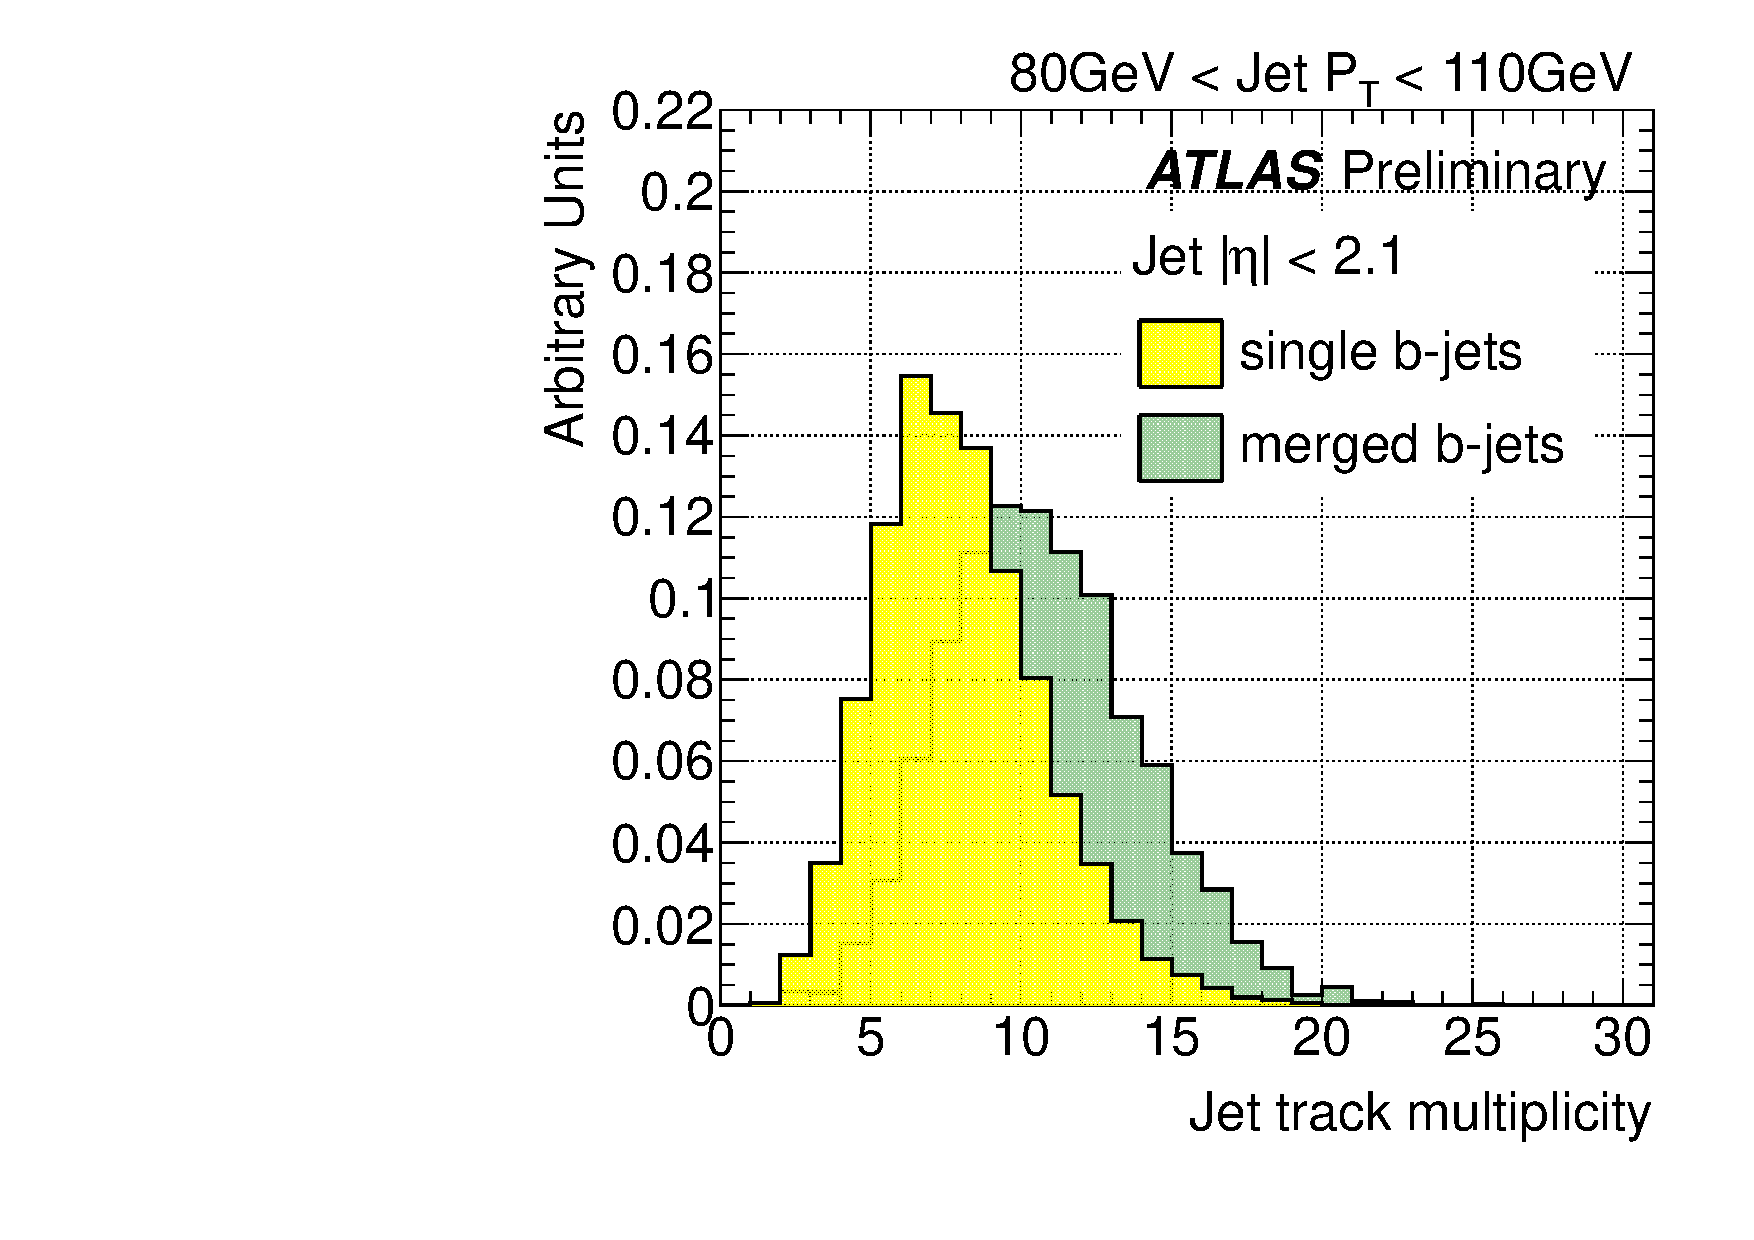
\includegraphics[width=0.49\textwidth]{FIGS/VarsSingleMerged/Ntrk080.pdf}
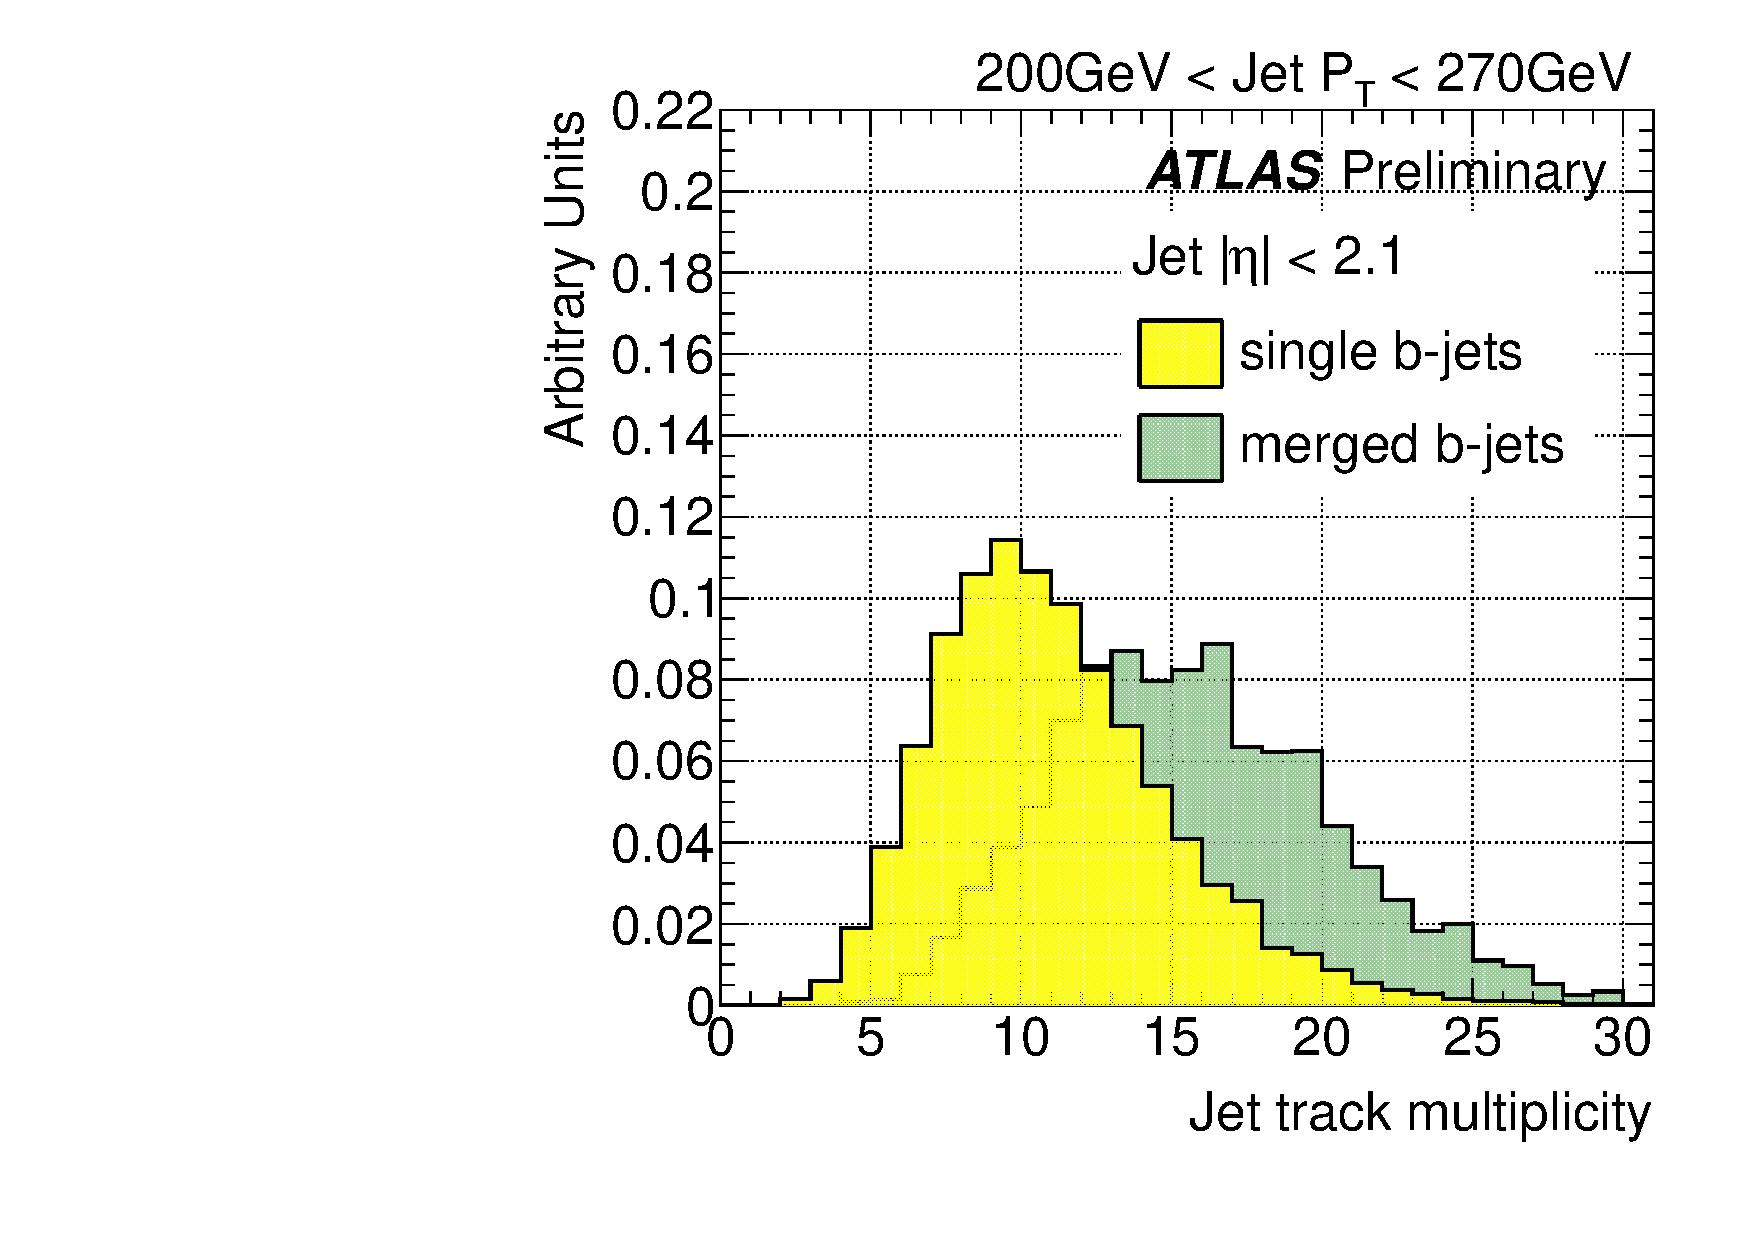
\includegraphics[width=0.49\textwidth]{FIGS/VarsSingleMerged/Ntrk200.pdf}
\caption{Distribution of the track multiplicity in jets for single and merged $b$-jets between 80~GeV to 110~GeV (left) and 200~GeV to 270~GeV (right).}
\label{fig:ntrksinglemerged}
\end{figure}


In order to evaluate the effect of using displaced tracks originating from the $b$-hadrons decays a preliminary study was done using a sample of dijet events generated with {\sc Pythia} and with no detector simulation. For this study jets were reconstructed using all stable particles in the event, clustered with the anti-$k_t$ algorithm. The association of charged particles was done in the same way as with the full ATLAS simluation. Distributions of the track multiplicity built using all charged particles and using only charged particles coming from the $b$-hadron decay (``$b$-tracks'') are illustrated in  in Fig.~\ref{fig:ntrksinglemergedPYTHIA}. A better discrimination between single and merged $b$-jets is observed when using $b$-tracks only. The result obtained with {\sc Pythia} suggests that a potential improvement in single-merged separation can be achieved by circumscribing the track selection, in the full simluation, to tracks with large impact parameter significance. % ($> 2.5$).
 A comparison of track multiplicity distributions using all tracks and distributions built with displaced tracks is shown in Fig.~\ref{fig:displacedntrk}. No improvement is obtained by using displaced tracks ($|d_0|/\sigma(d_0)> 2.5$). The potential sensitivity achieved by enriching the sample in tracks associated to the $b$-hadron is counterbalanced by the lower number of associated tracks.
%\vspace{3 mm}

\begin{figure}[tp]
\centering
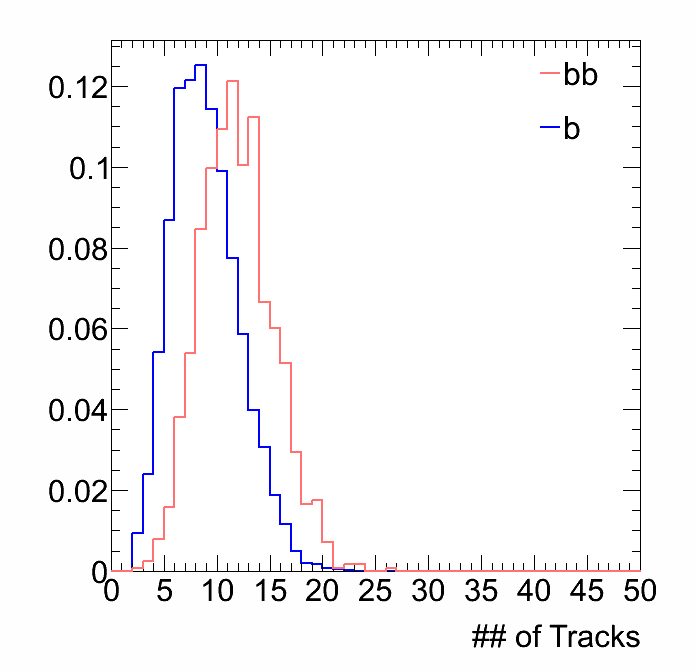
\includegraphics[width=0.49\textwidth]{FIGS/TEMPFigs/PythisStandalone/MaxPlots/ntrk_gbb_b_J3_PT80.png}
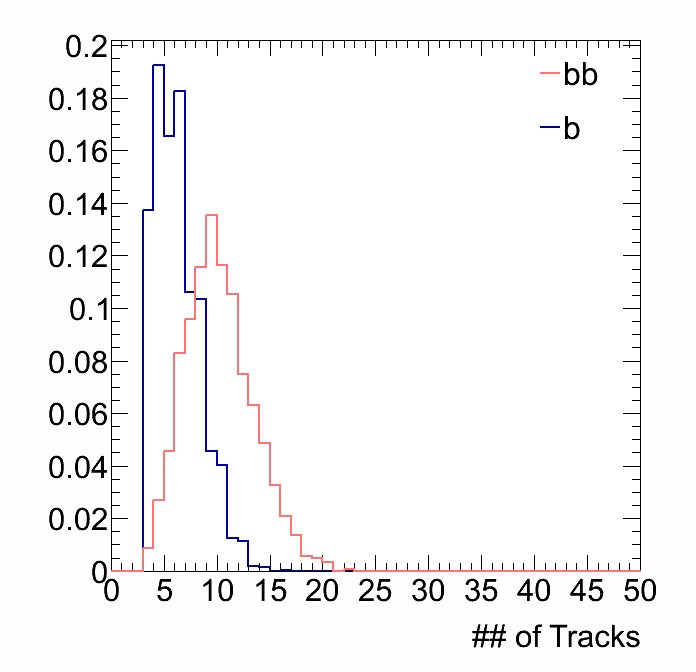
\includegraphics[width=0.49\textwidth]{FIGS/TEMPFigs/PythisStandalone/MaxPlots/ntrkB_gbb_b_J3_PT80.png}
\caption{Distribution of the track multiplicity in jets for single ($b$) and merged ($bb$) jets between 80~GeV to 120~GeV in a sample of dijet events generated with {\sc Pythia} and no detector simulation. Distributions are shown using all charged particles (left) and using only charged particles coming from $b$-hadron decay (right).}
\label{fig:ntrksinglemergedPYTHIA}
\end{figure}

\begin{figure}[tp]
\centering
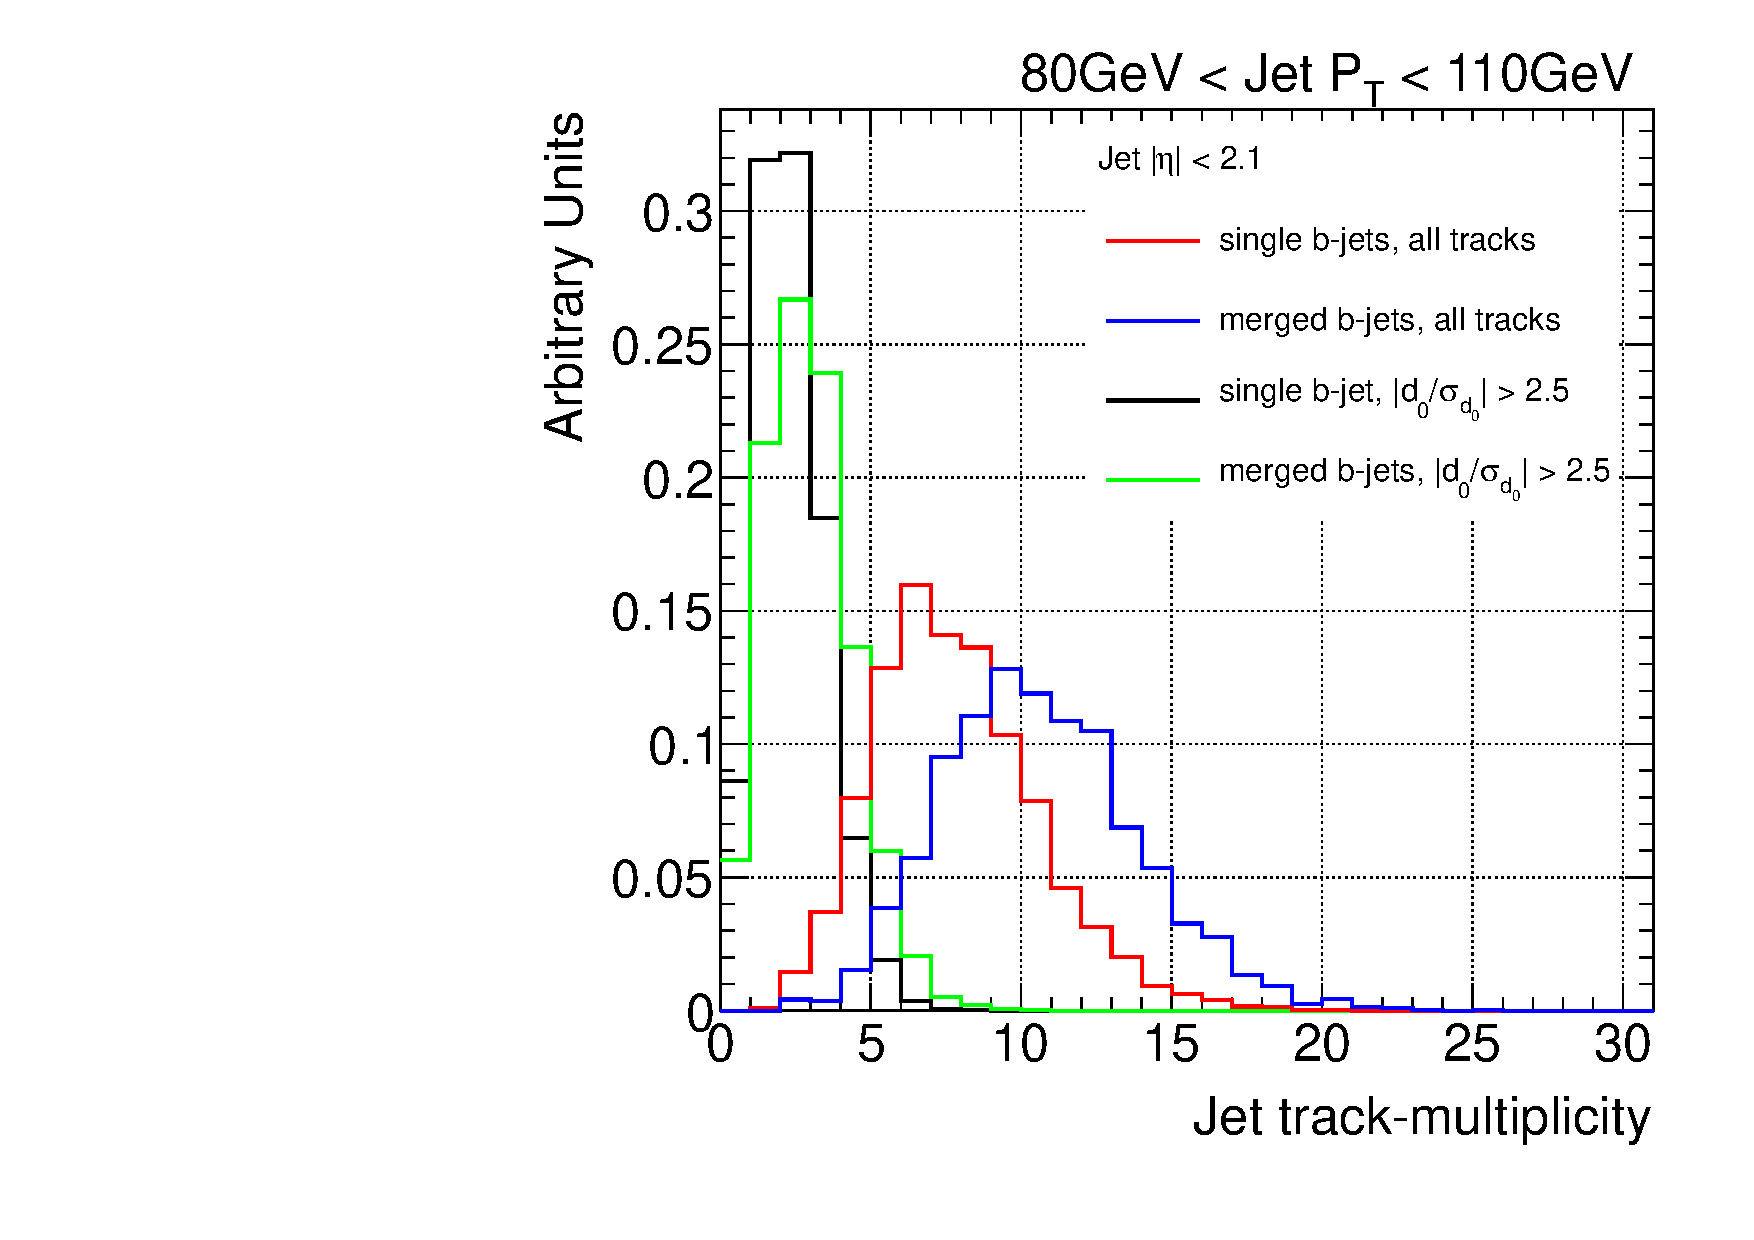
\includegraphics[width=0.49\textwidth]{FIGS/TEMPFigs/DisplacedTracks/Ntrk_allanddisplacedW080.pdf}
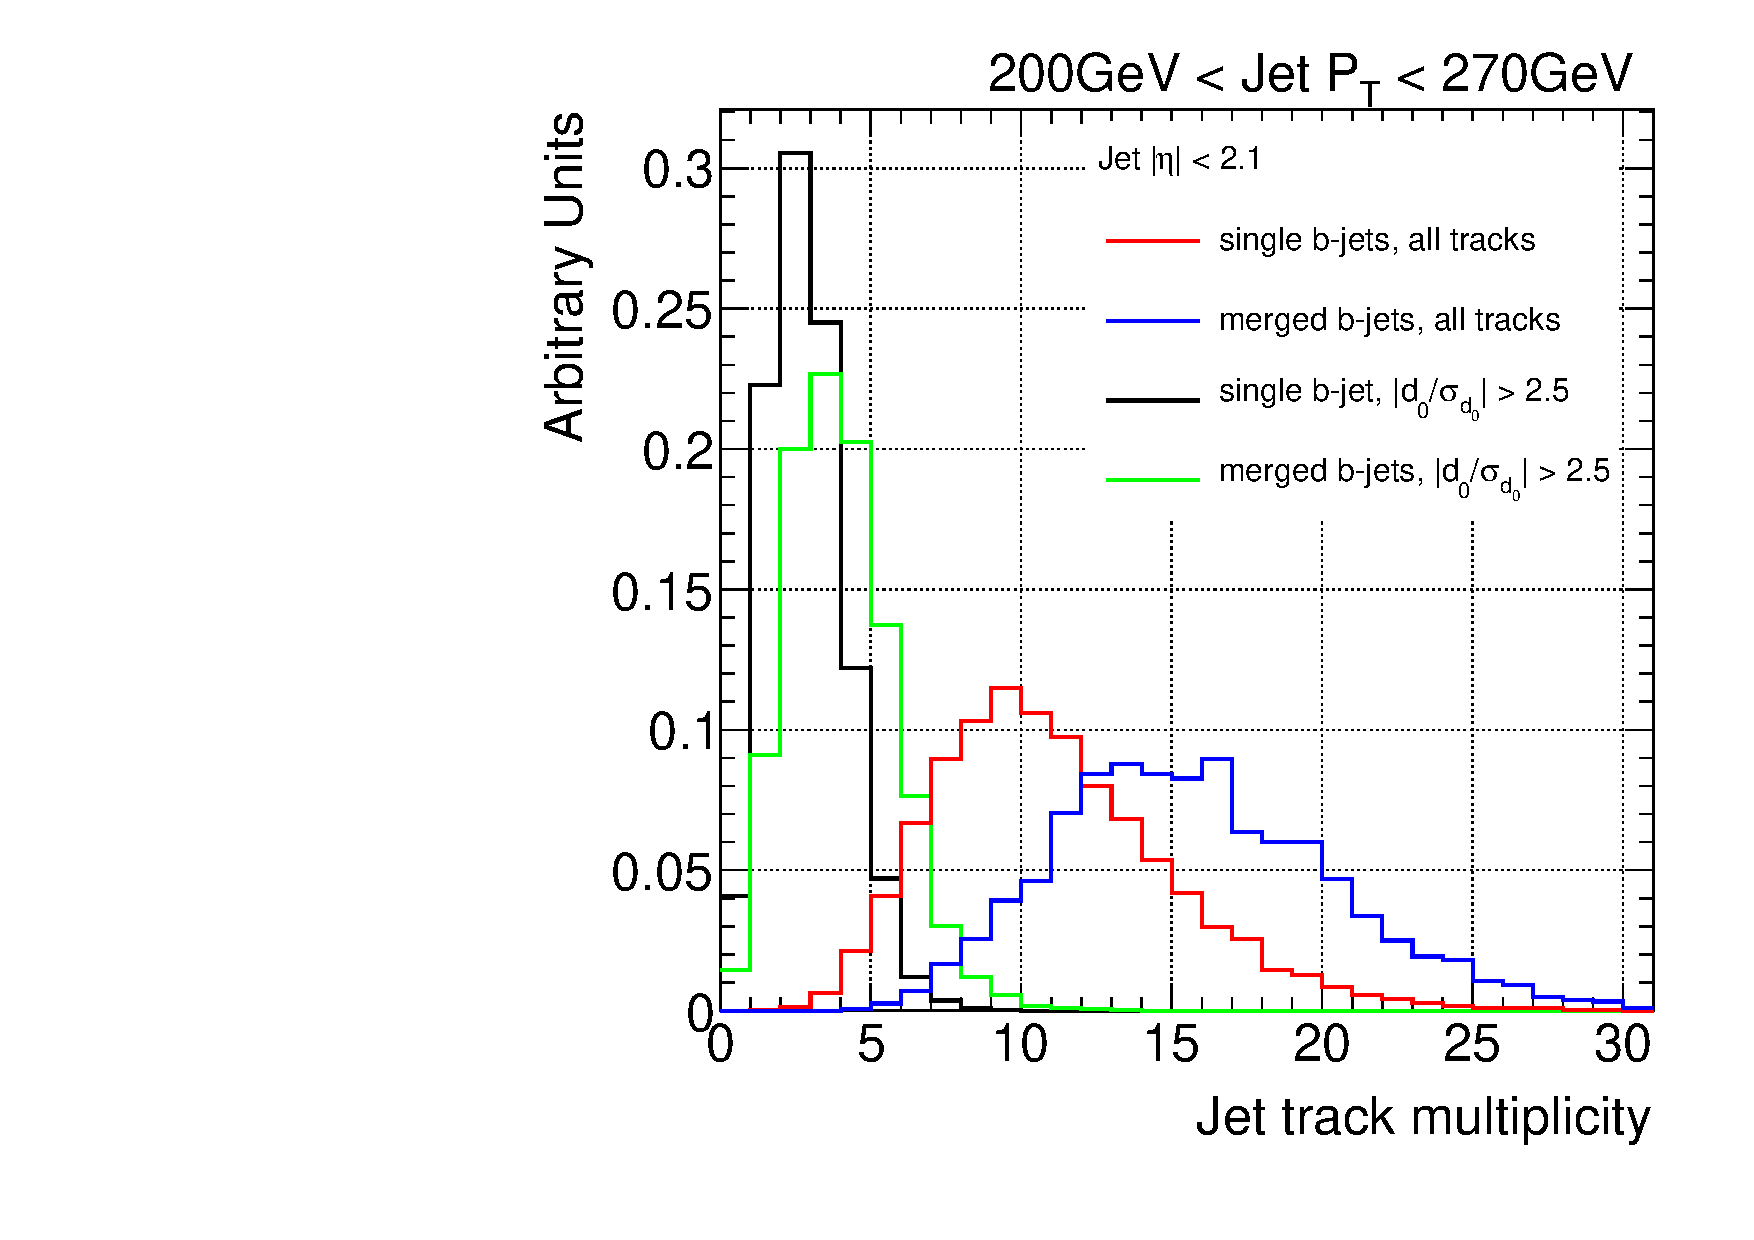
\includegraphics[width=0.49\textwidth]{FIGS/TEMPFigs/DisplacedTracks/Ntrk_allanddisplacedW200.pdf}
\caption{Distribution of the jet track multiplicity single and merged $b$-jets between 80~GeV to 110~GeV (left) and 200~GeV to 270~GeV (right), for all and displaced tracks only.}
\label{fig:displacedntrk}
\end{figure}


%\begin{figure}[tp]
%\centering
%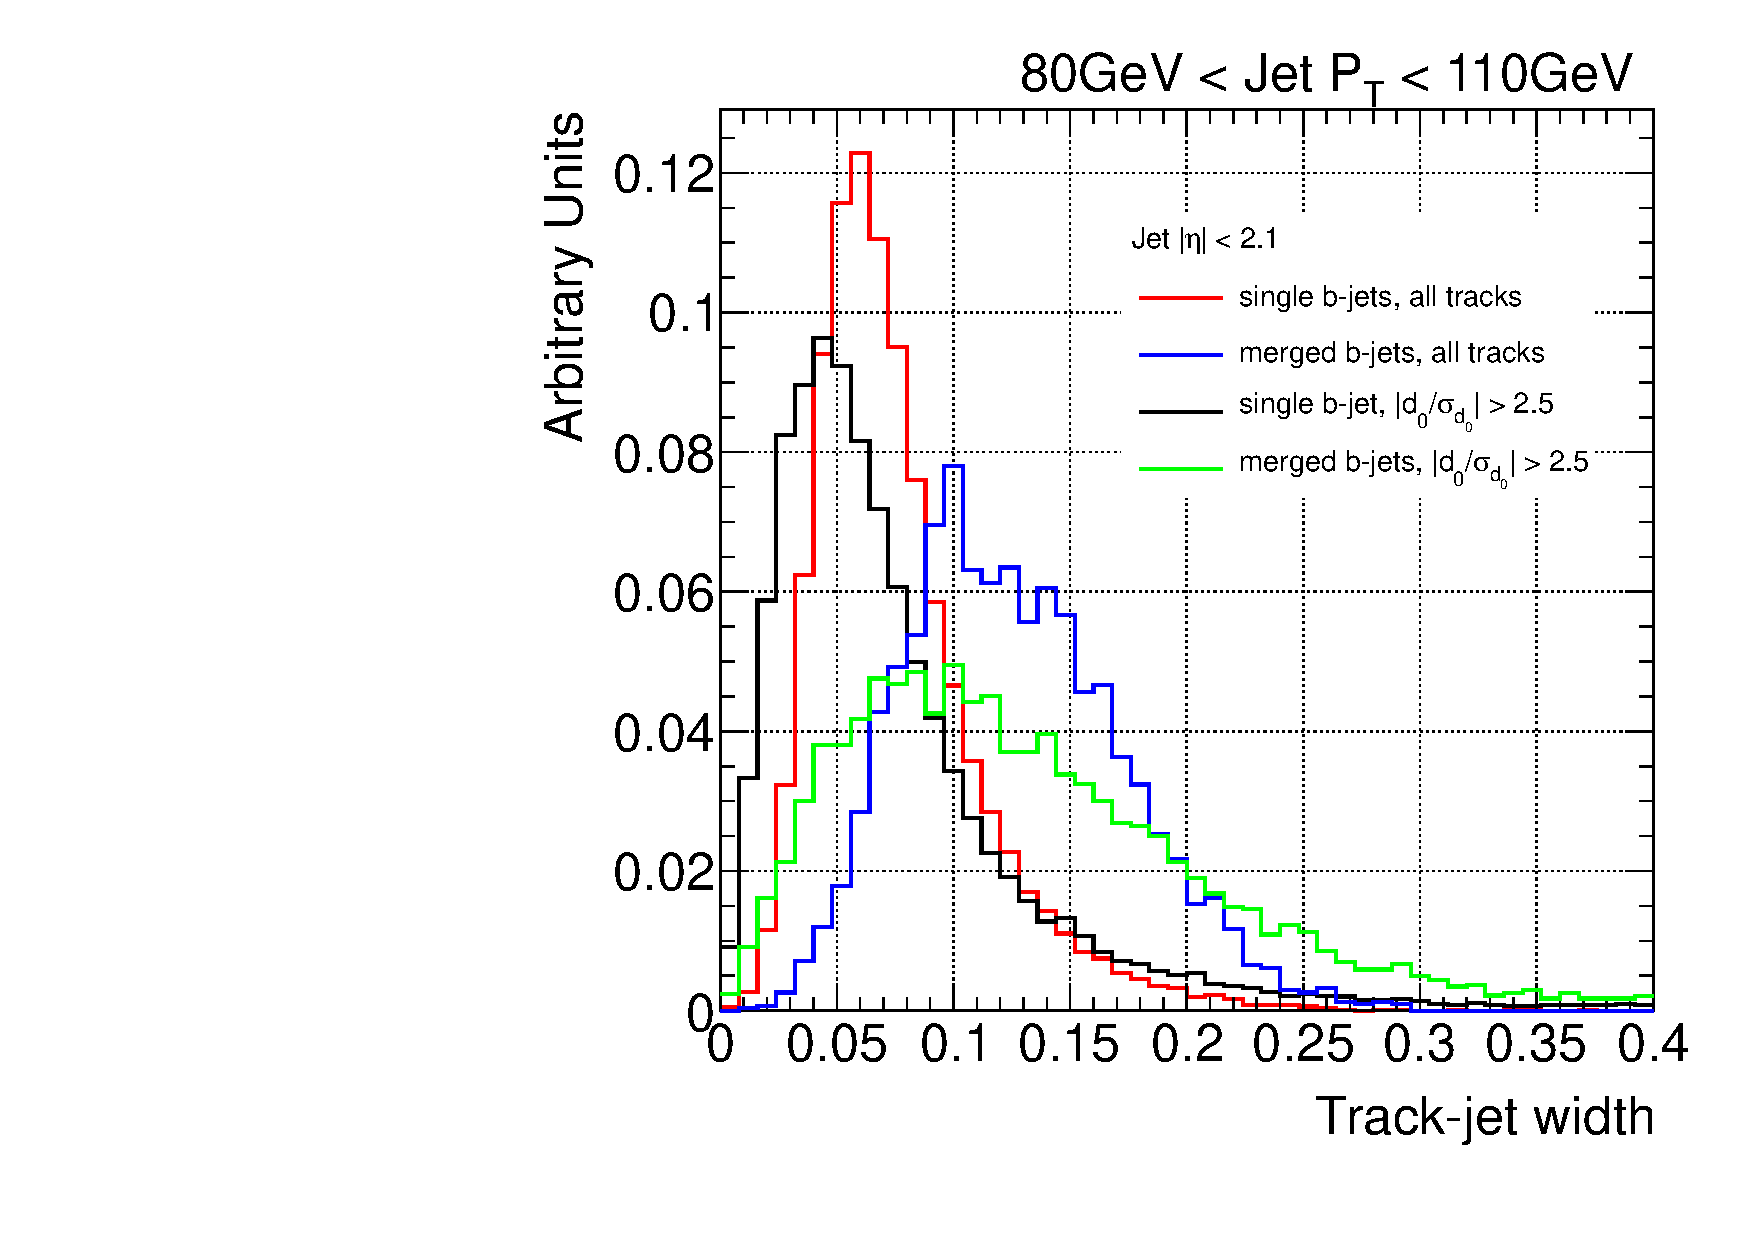
\includegraphics[width=0.49\textwidth]{FIGS/TEMPFigs/DisplacedTracks/trkWidth_allanddisplaced080.pdf}
%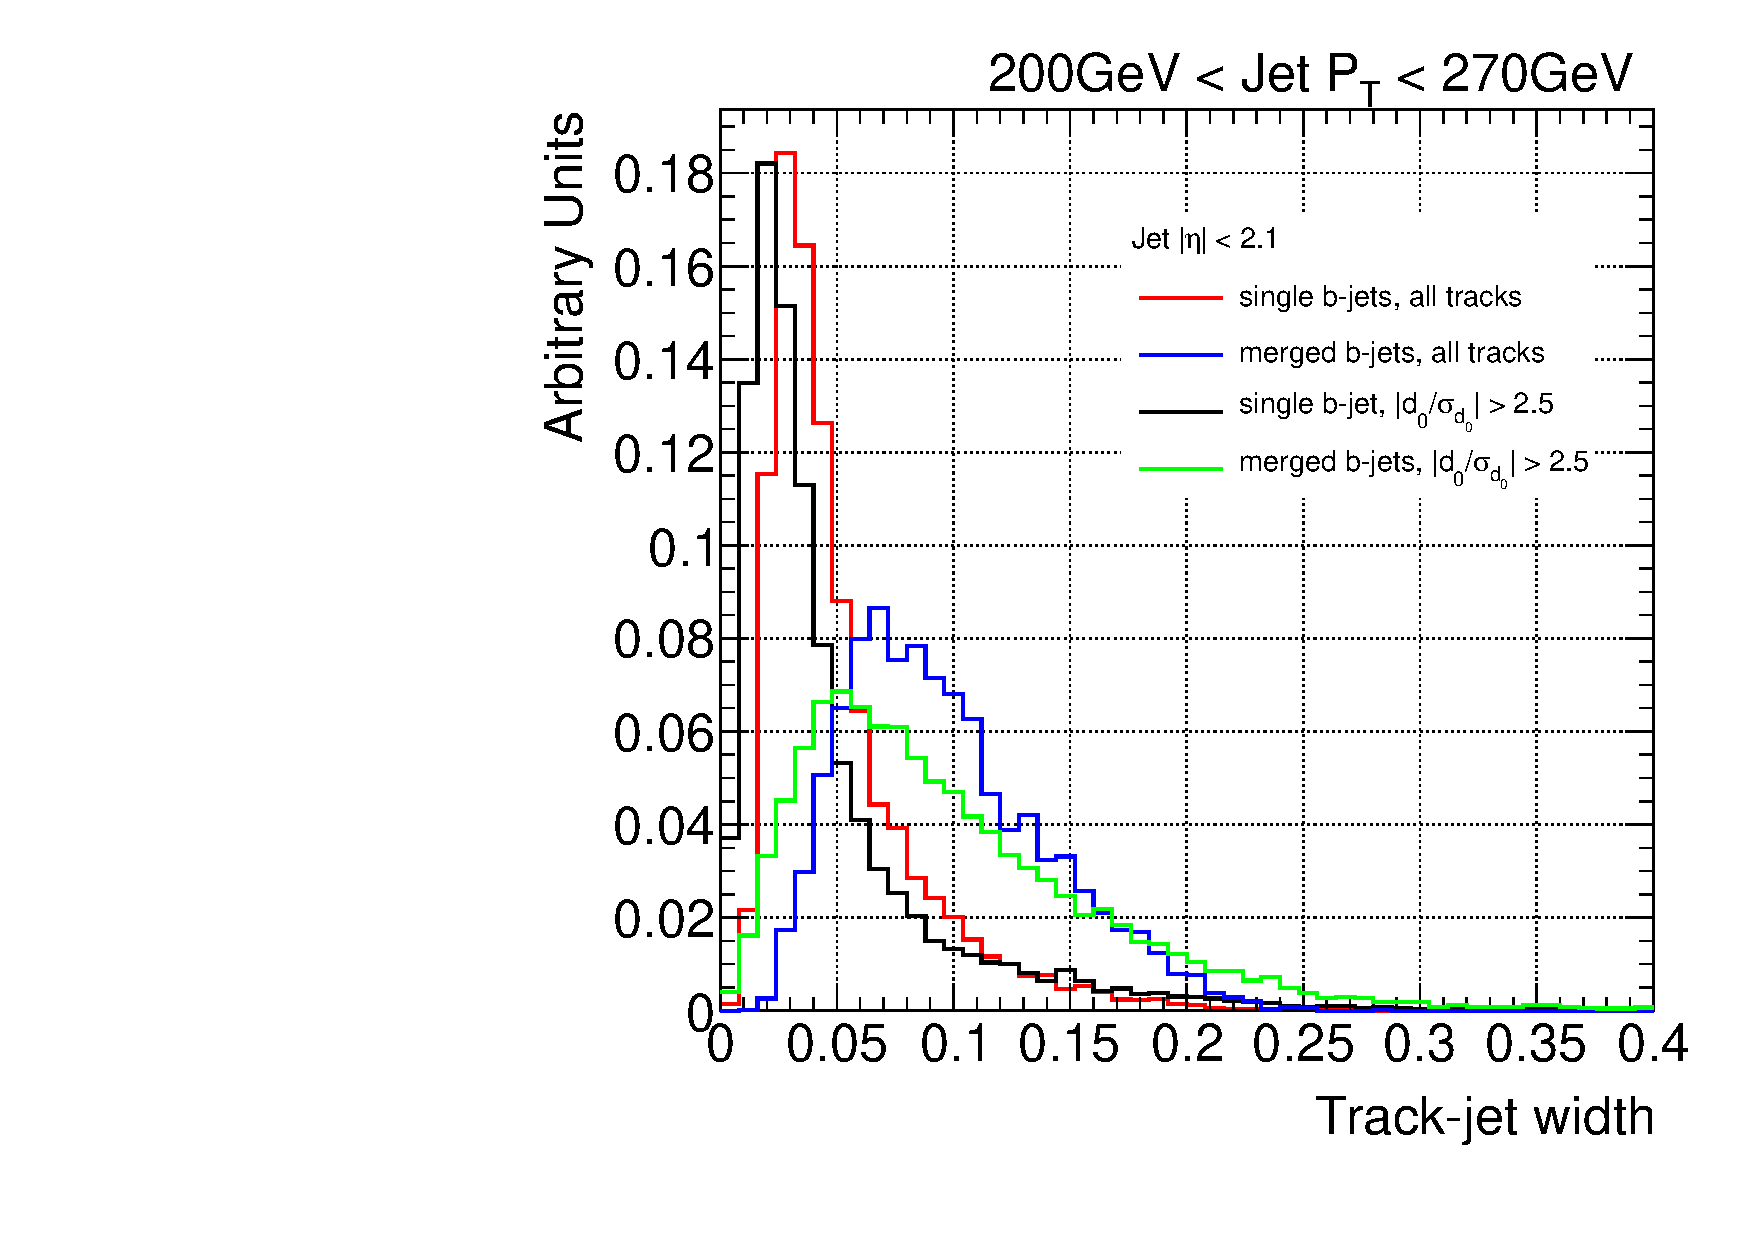
\includegraphics[width=0.49\textwidth]{FIGS/TEMPFigs/DisplacedTracks/trkWidth_allanddisplaced200.pdf}
%\caption{Distribution of the track-jet width for single and merged $b$-jets between 80~GeV to 110~GeV (left) and 200~GeV to 270~GeV (right), for all and displaced tracks only.}
%\label{fig:displacedtrkwidth}
%\end{figure}

%There is a small number of jets at low pt that have only one track, because the selection criteria are not identical to those applied at the moment of b-tagging. Shape variables are not calculated for these jets, which are directly classified as single in the tagger presented in section 8. 



%%%%%%%%%%%%%%%%%%%%%%%%%%%%%%%%%%%%%%%%%%%%%%%%%%%%%%%%%%%%%%%%%%%%%%%%%%%%%%%%%%%%%%%
%{ \em II. Jet width}
%\vspace{3 mm}
%This linear radial moment is a measure of the width or ``girth''~\cite{PhysRevLett.105.022001} of the jet.  Under the assumption of central jets with massless constituents at small angles, this linear moment is identical to jet broadening~\cite{Catani1992269}, defined as the sum of momenta transverse to the jet axis normalized by the sum of momenta. While jet broadening is natural at an $e^+ e^-$ collider, the linear radial moment is more natural at the LHC.

{ \em Jet width} The jet width is part of a set of continuous variables that try to distinguish individual particles/subjets within the jet by means of smooth funcion of $(\Delta \eta, \Delta \phi)$ away from the jet axis, in order to form combinations like geometric moments.  This particular combination is a linear moment which sums the distances between the jet constituents and its axes, weighted by the constituent $\pt$, and then normalized to the total $\pt$ of the jet.  Its definition is,
%
\begin{equation} 
\mbox{ {\it Jet width}} = \frac{\sum_{i=1}^N \pt^{const_i} \,\Delta R (const_i,jet) }{\sum_{i=1}^N \pt^{const_i} }
\label{eqn:trackjetwidth}
\end{equation} 
%
where $N$ is the total number of calorimeter or track constituents.  %This observable is also highly correlated to the mass of the jet.

This observable has been extensively used to discriminate between gluon initiated and light quark initiated jets, see for instance~\cite{PhysRevLett.107.172001} and~\cite{ATLAS-CONF-2011-053}. Gluon jets are seen to be broader than quark jets. In the case of jets originating from $b$-quarks, these resemble gluon jets more closely than quarks jets~\cite{Buskulic1996353}: due to the longer decay chain of $b$-hadrons the angular spread is larger for a $b$-jet than a light-quark jet. In order to explore how merged jets, originating from a gluon splitting into a $b\bar{b}$ pair, compare to single $b$-quark jets and pure gluon jets,  a standalone {\sc Pythia} analysis was performed.  Figure~\ref{fig:trkwidthsinglemergedPYTHIAgluon} illustrates the result; $b$-jets containing two $b$-hadrons present a greater angular width relative to single $b$-jets and gluon initiated jets. The latter, in turn, looks broader than single for medium $\pt$ jets. This behavior is somehow expected in the LHC's higher $\pt$ jets because the QCD shower produces more particles resulting in broader gluon jets,  whereas the particle multiplicity is relatively fixed in the $b$-hadron decay.

Distributions for the track-jet width with full ATLAS simulation are shown in Fig.~\ref{fig:trkwidthsinglemerged}. In this case % for which 
the sum in equation~\ref{eqn:trackjetwidth} runs over the $N$ tracks associated to the jet, using the same criteria as for the jet track multiplicity. As expected, merged $b$-jets are wider than single $b$-jets. 

{\sc Pythia} standalone samples were also to used evaluate the potential gain in discrimination obtained by utilising all stable particles in the event to build the observable, as opposed to using the charged particles only.  A 10\% %HACER CALCULO!!!!
 improvement in merged $b$-jet rejection (for a 50\% efficiency in selecting single $b$-jets) was achieved.

In full simulation, the jet width can be measured in terms of calorimeter variables by replacing tracks by topological clusters in the sum.  Although it offers good separation, this variable is more sensitive to the amount of pile-up in the event than its track-based counterpart. This is illustrated in Fig.~\ref{fig:trkwidthpileup}, which shows the distribution of calorimeter width and track-jet width for single $b$-jets in events with low and high number of primary vertices (NPV) in a low $\pt$ region where the effect of pile-up is more important. 

 In general, all the studied calorimeter-based jet variables show similar dependences with NPV. For this reason the track-based versions are preferred as more robust discriminators.
%\vspace{3 mm}


\begin{figure}[tp]
\centering
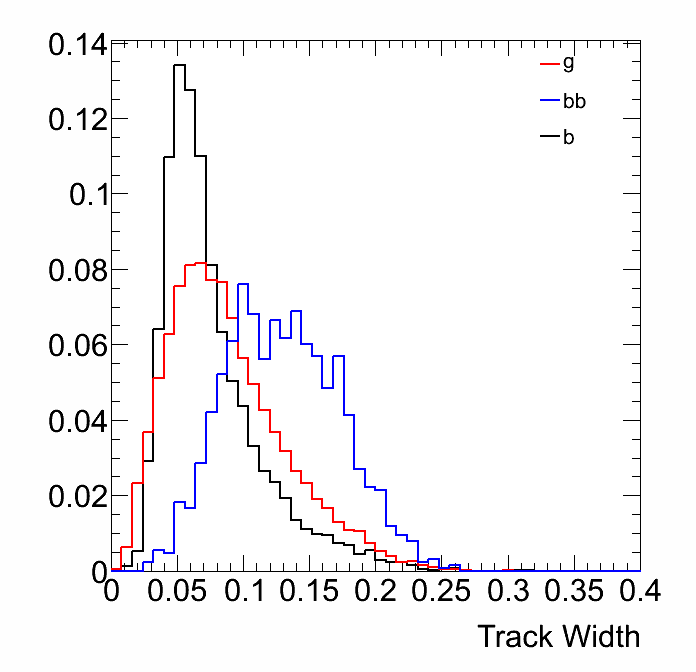
\includegraphics[width=0.49\textwidth]{FIGS/VarsSingleMerged/trkWidth_bb_b_g_J3_PT80.png}
%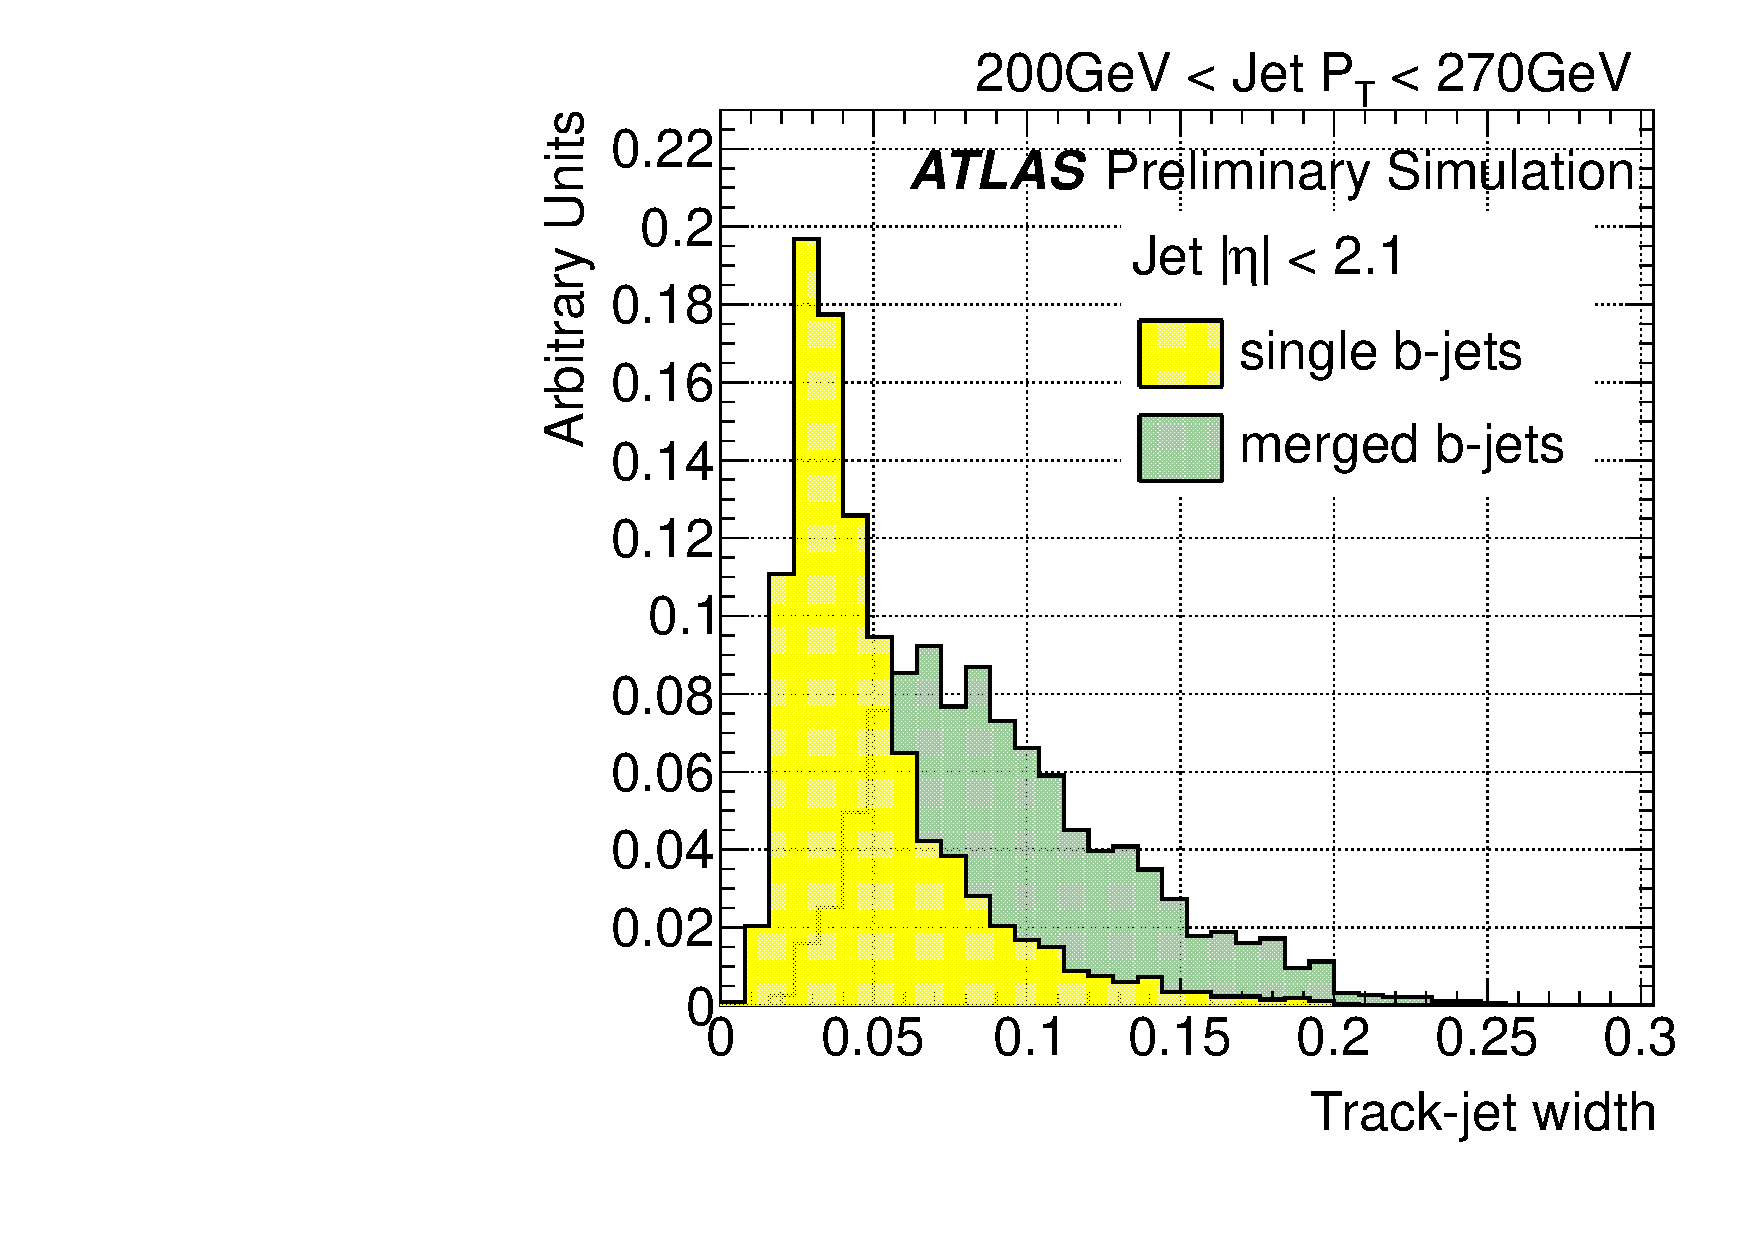
\includegraphics[width=0.49\textwidth]{FIGS/VarsSingleMerged/trkWidth200.pdf}
\caption{Distribution of track-jet width in jets for gluon-initiated ($g$), single ($b$) and merged ($bb$) jets between 80~GeV to 120~GeV in a sample of dijet events generated with {\sc Pythia} and no detector simulation.}
\label{fig:trkwidthsinglemergedPYTHIAgluon}
\end{figure}

\begin{figure}[tp]
\centering
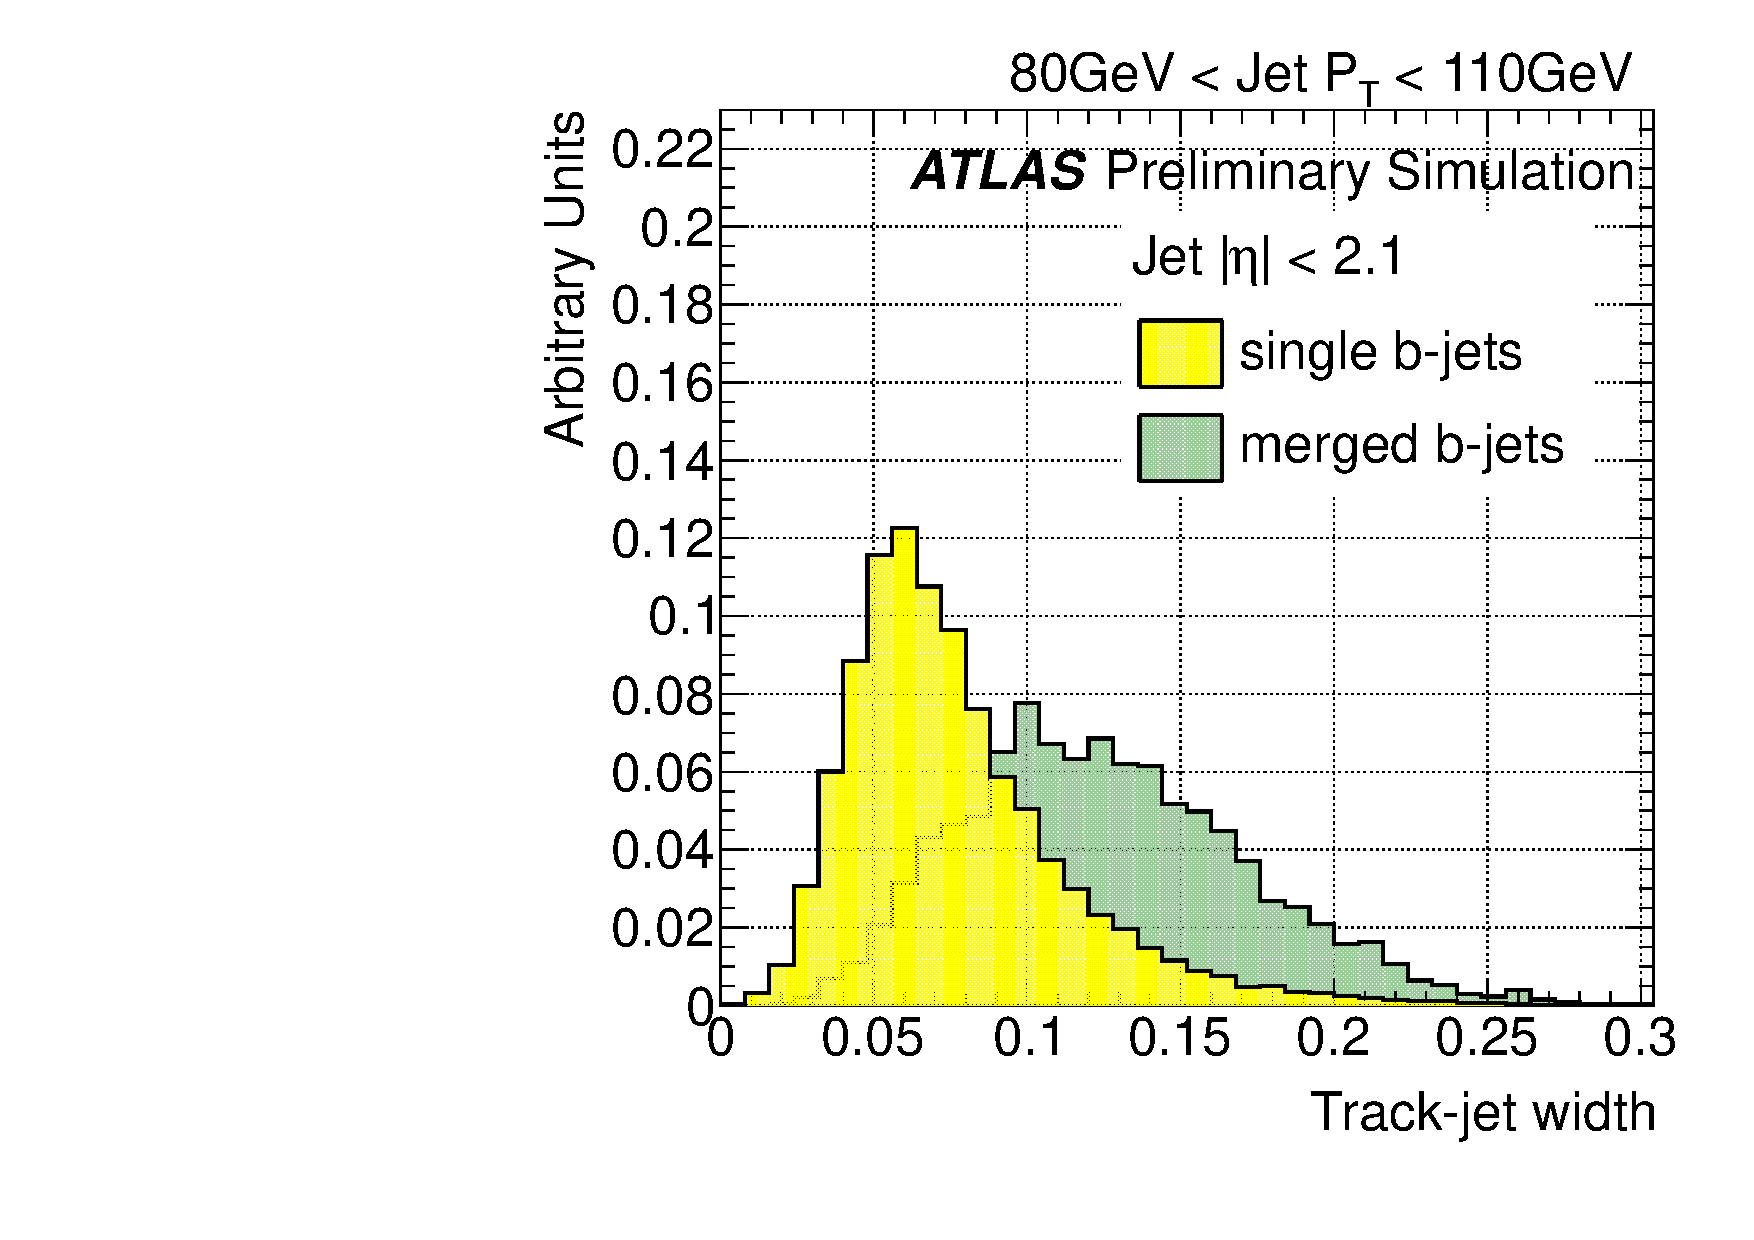
\includegraphics[width=0.49\textwidth]{FIGS/VarsSingleMerged/trkWidth080.pdf}
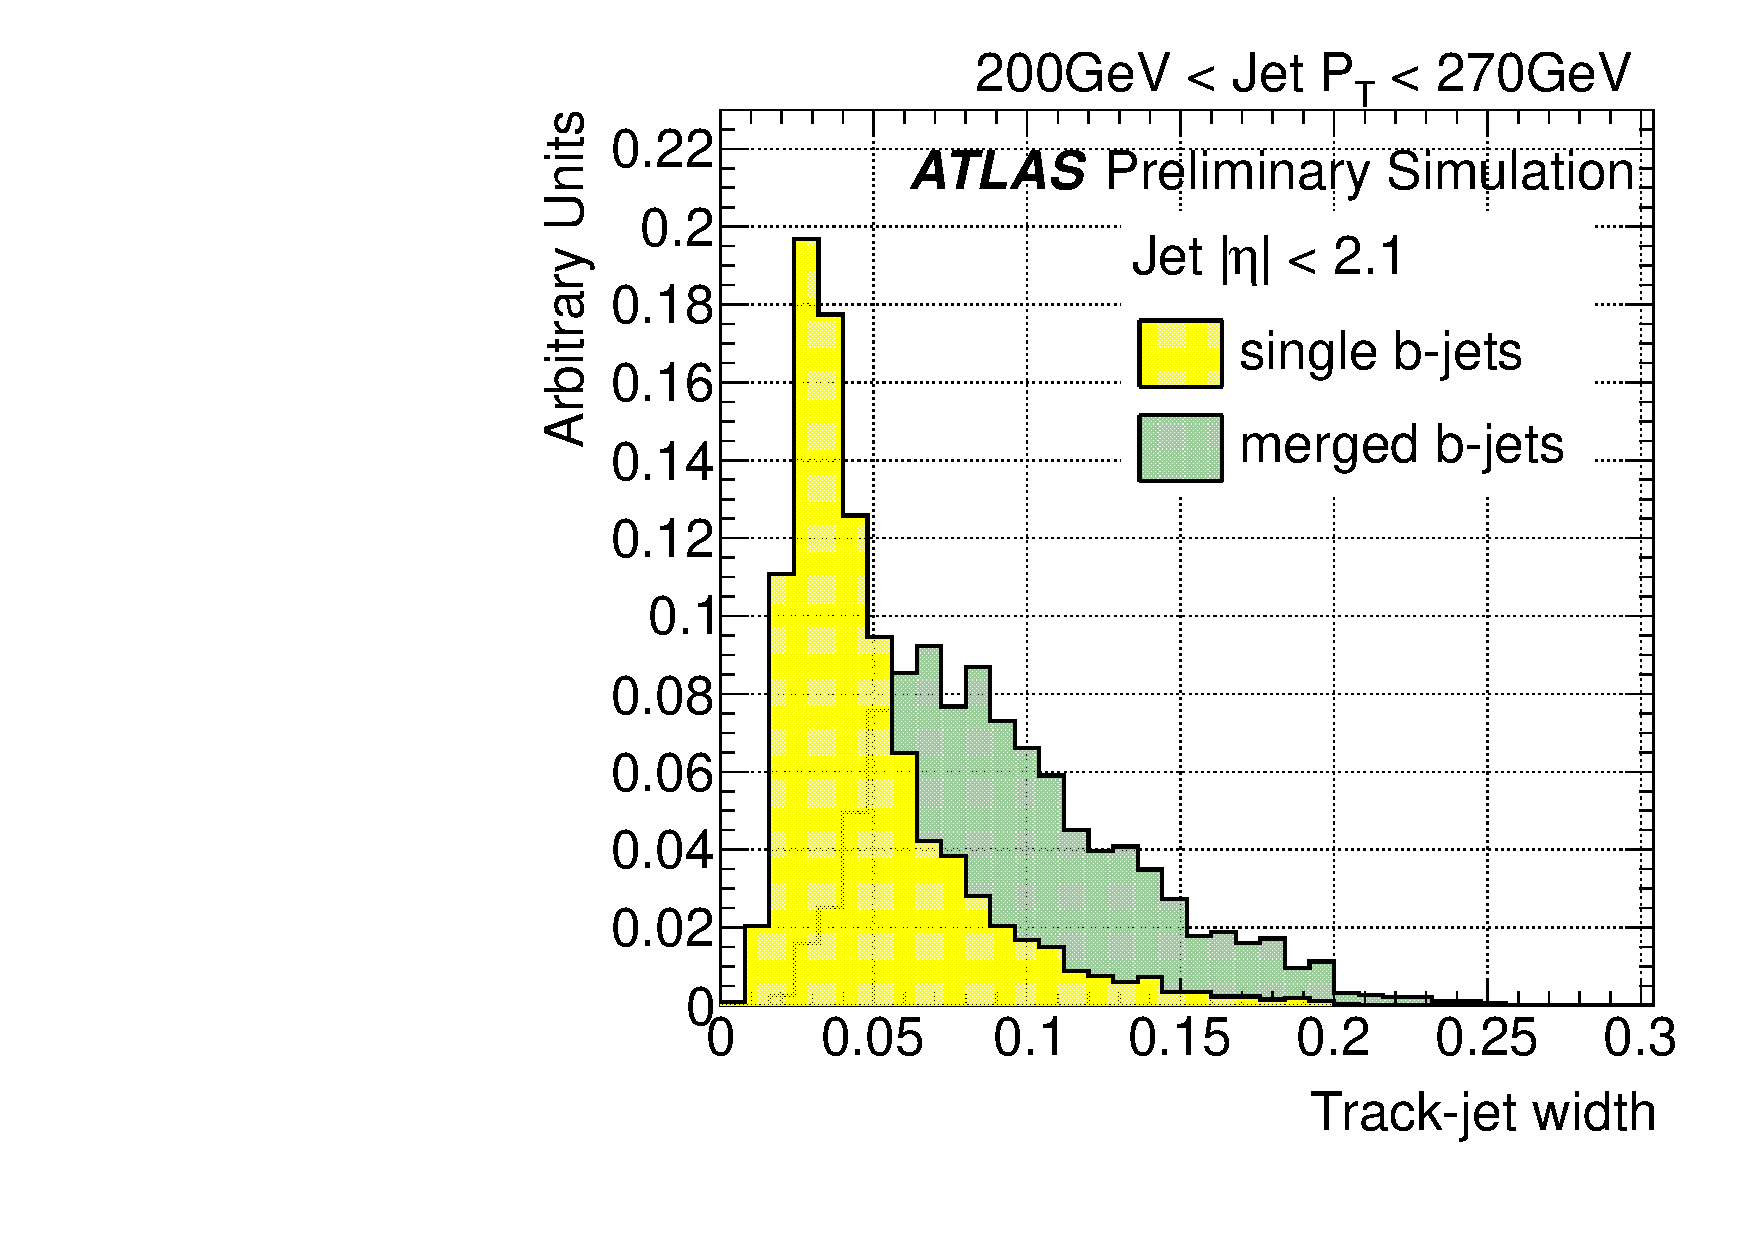
\includegraphics[width=0.49\textwidth]{FIGS/VarsSingleMerged/trkWidth200.pdf}
\caption{Distribution of track-jet width in jets for single and merged $b$-jets between 80~GeV to 110~GeV (left) and 200~GeV to 270~GeV (right).}
\label{fig:trkwidthsinglemerged}
\end{figure}


%\begin{figure}[tp]
%\centering
%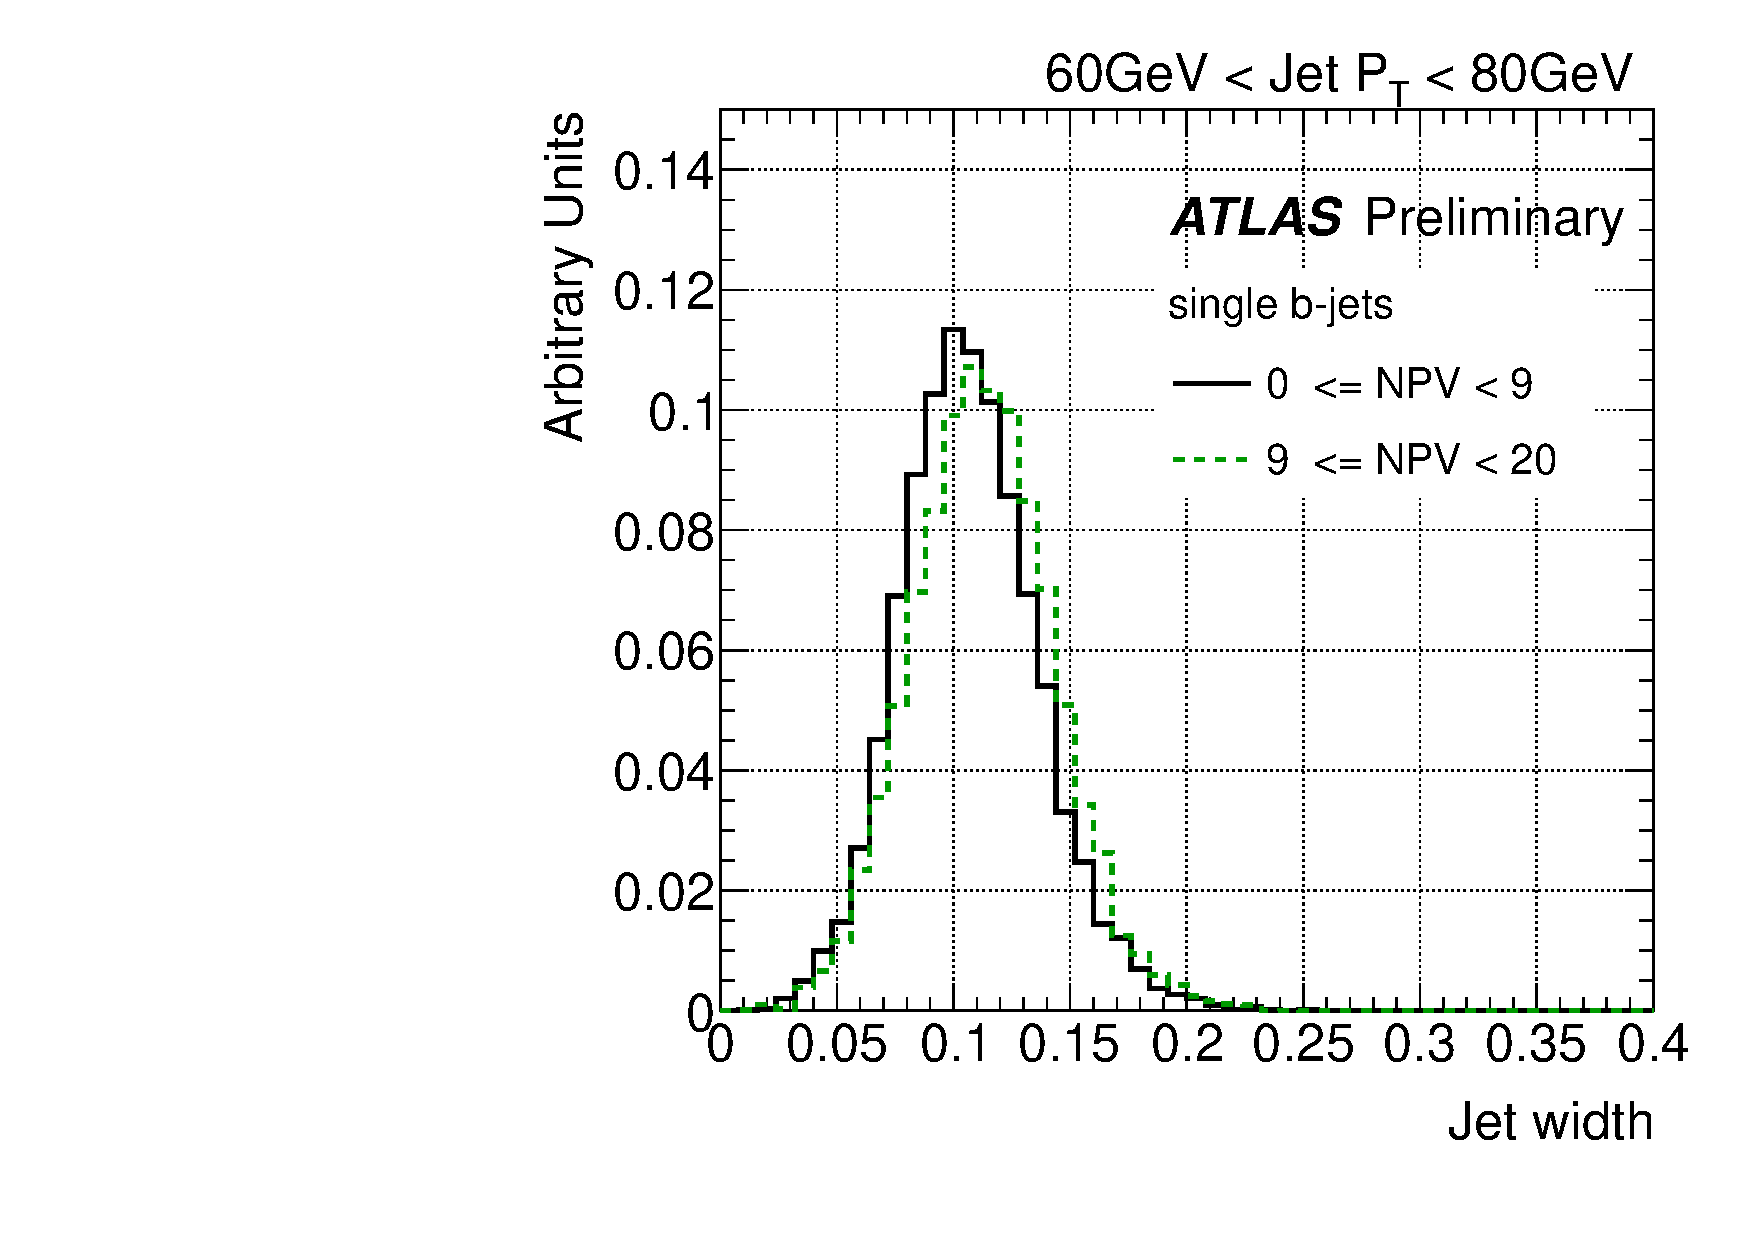
\includegraphics[width=0.49\textwidth]{FIGS/systematics/Widthsingle_060.pdf}
%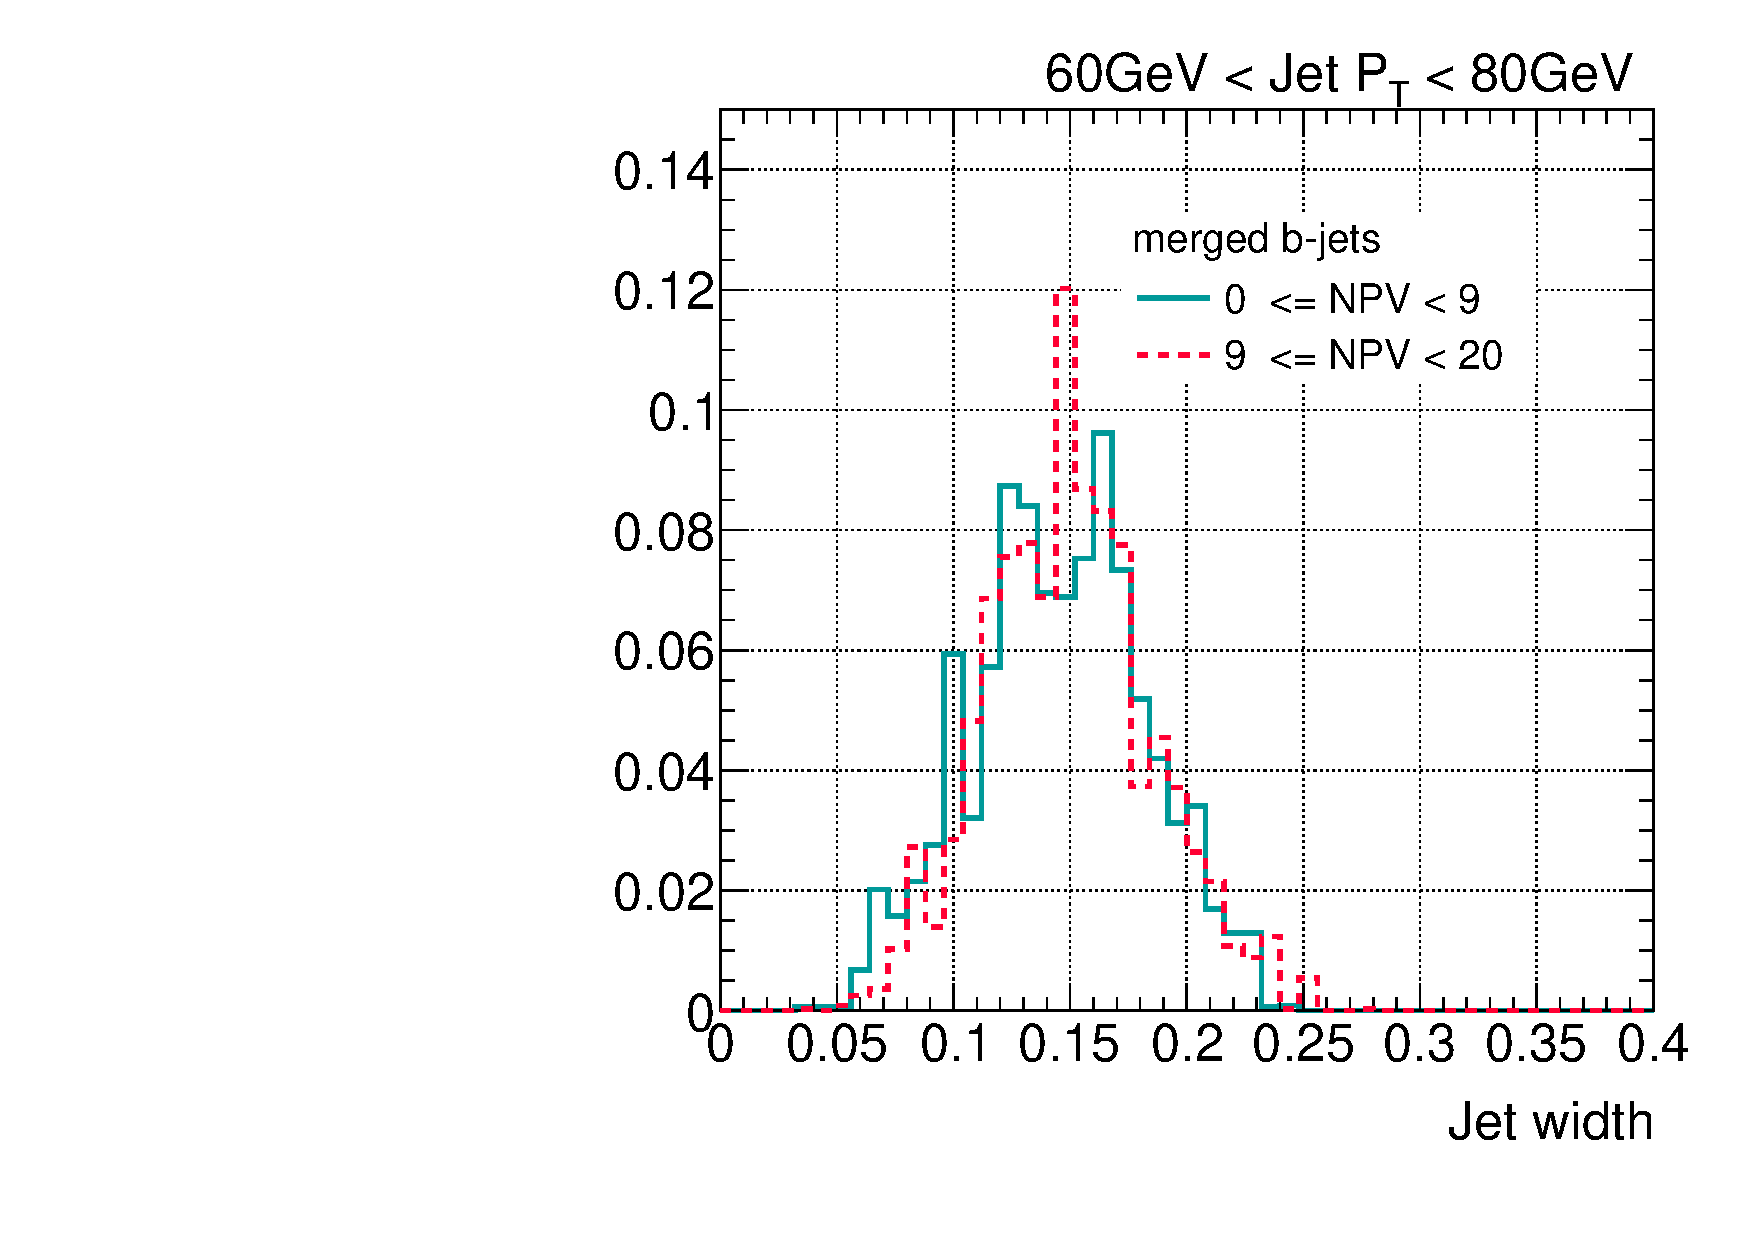
\includegraphics[width=0.49\textwidth]{FIGS/systematics/Widthmerged_060.pdf}
%\caption{Distribution of calorimeter jet width (using topological clusters) for single (left) and merged (right) $b$-jets in two bins of Number of Primary Vertices for jets between 60~GeV to 80~GeV.}
%\label{fig:calowidthpileup}
%\end{figure}
\begin{figure}[tp]
\centering
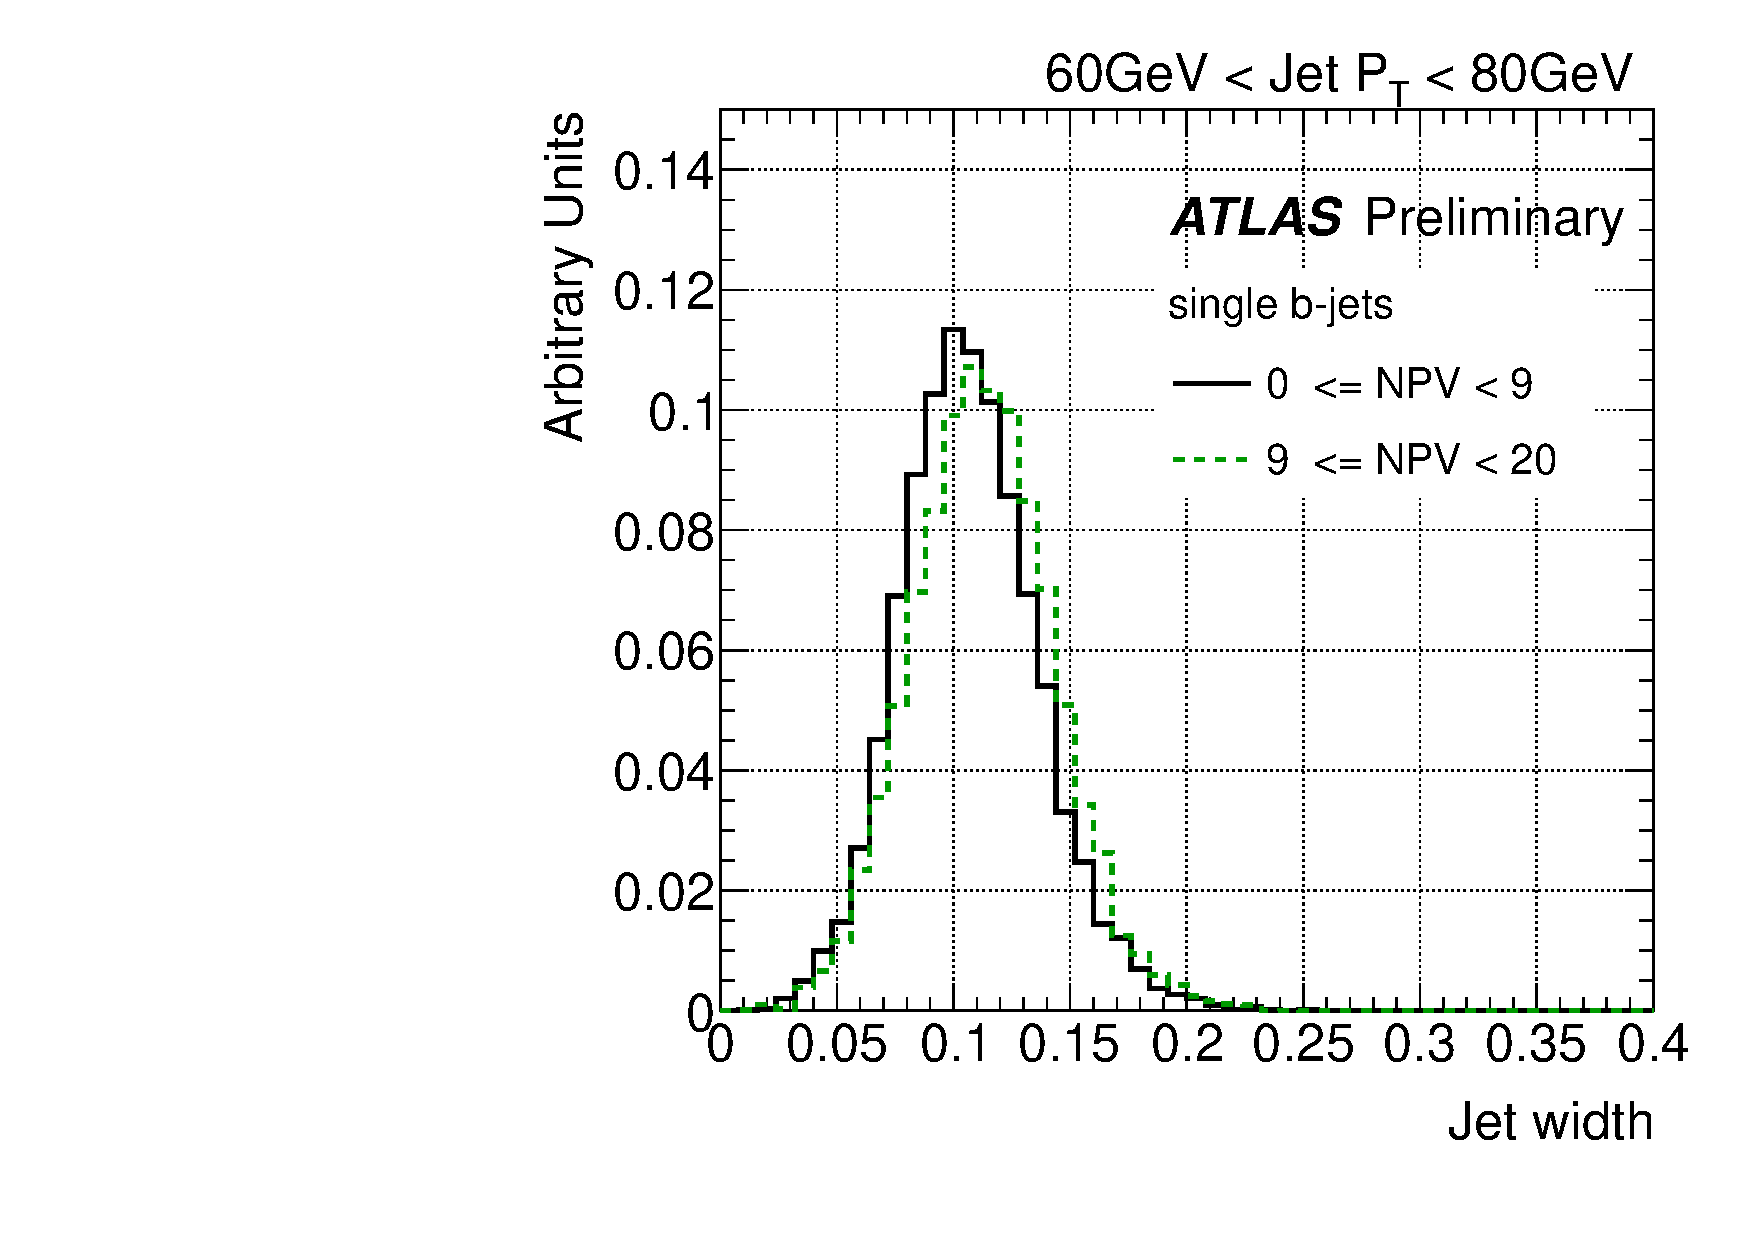
\includegraphics[width=0.49\textwidth]{FIGS/systematics/Widthsingle_060.pdf}
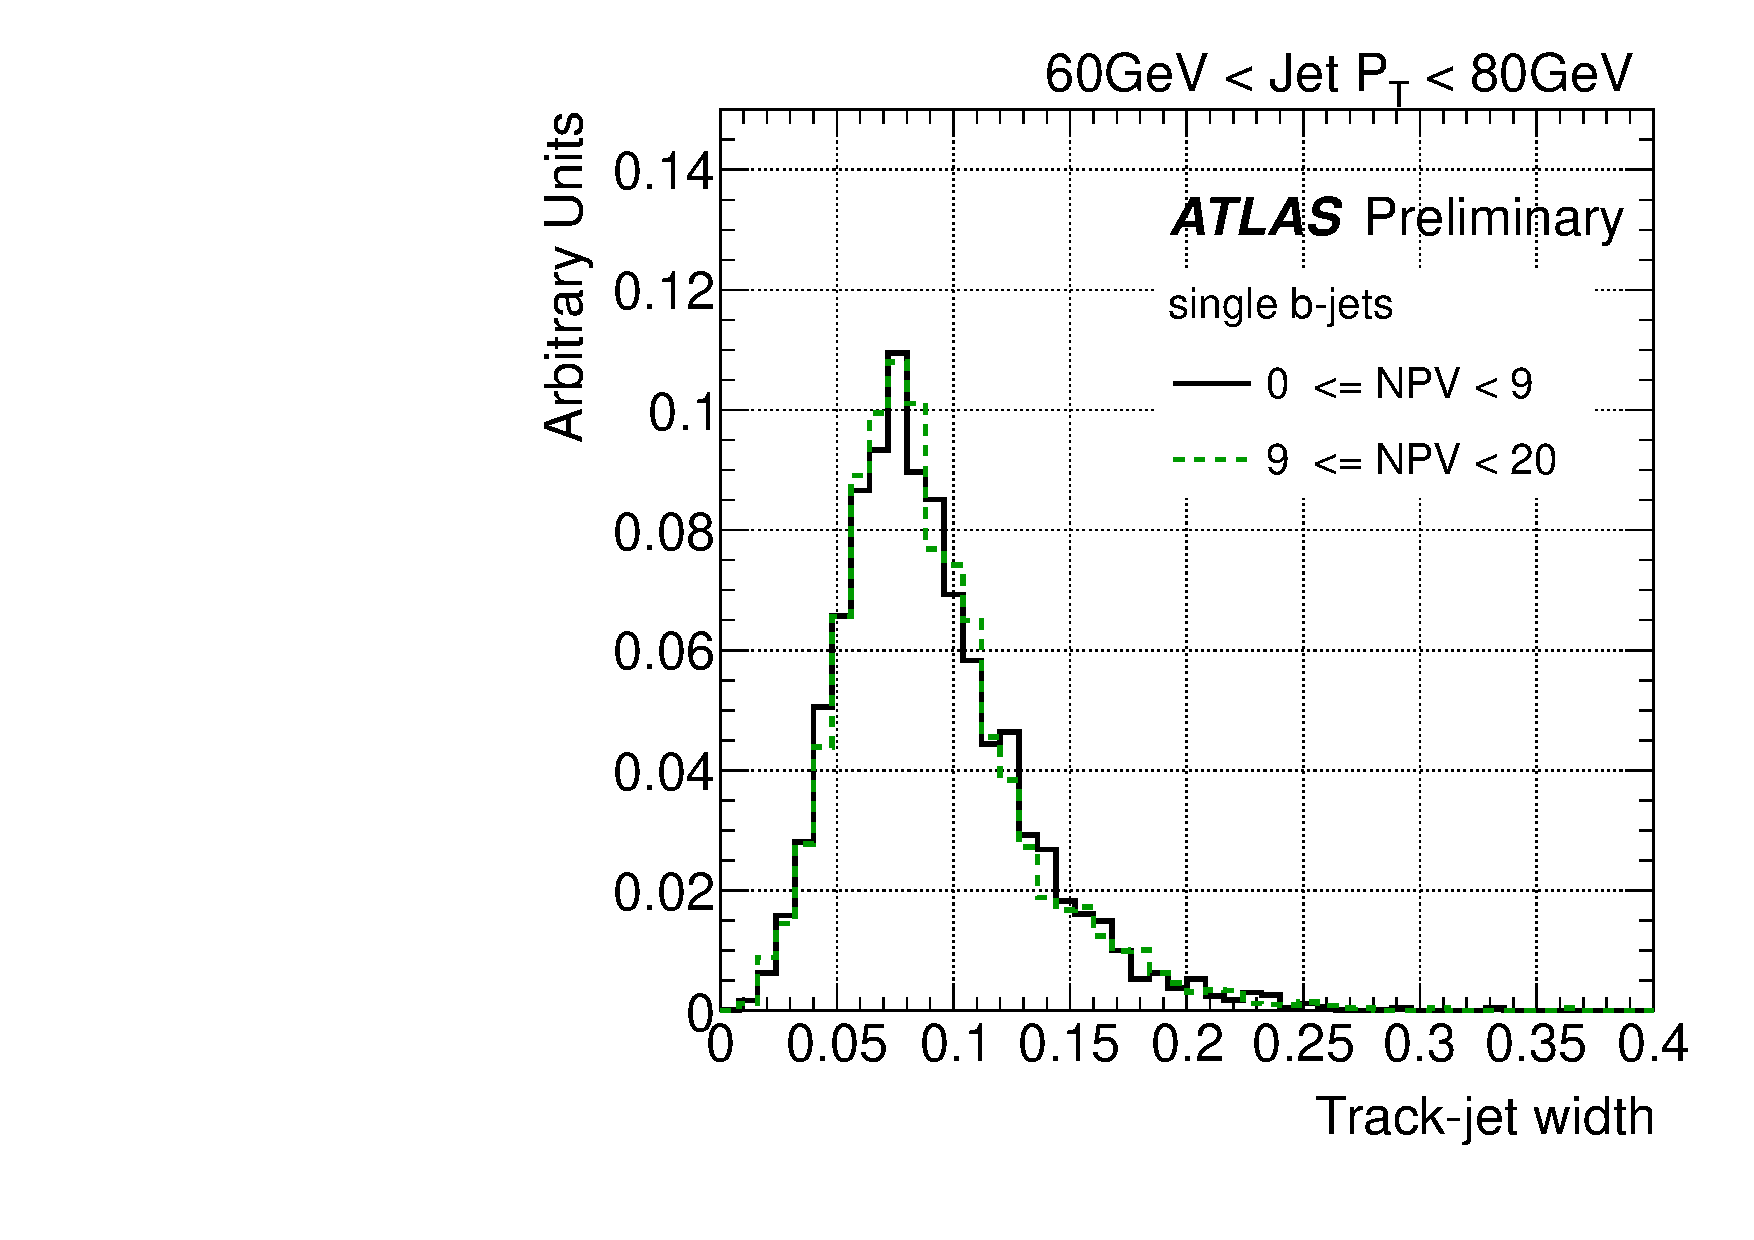
\includegraphics[width=0.49\textwidth]{FIGS/systematics/trkWidthsingle_060.pdf}
\caption{Distribution of jet width using topological clusters (left) and tracks (right) for single $b$-jets in two bins of number of primary vertices (NPV) for jets between 60~GeV to 80~GeV.}
\label{fig:trkwidthpileup}
\end{figure}

%%%%%%%%%%%%%%%%%%%%%%%%%%%%%%%%%%%%%%%%%%%%%%%%%%%%%%%%%%%%%%%%%%%%%%%%%%%%%%%%%%%%%%%%%%%%%%
%{ \em III. Jet Mass}
%\vspace{3 mm}

{ \em Jet Mass} The jet mass, like the linear radial moment, also depends on the radiation pattern of the event. It is the most basic observable for disinguishing massive boosted objects from jets originating from quarks or gluons. The latter are expected to be dominated by wide-angle emissions, with increase probability to see high mass jets initiated from gluons as opposed to quarks~\cite{PhysRevD.79.074012}.  
Figure~\ref{fig:masssinglemerged} shows the distribution of the jet mass for single and merged $b$-jets. Merged jets tend to have higher masses than single $b$-jets for the same $\pt$ bin. Although it shows good separation, this calorimeter based variable is susceptible to the amount of pile-up in the event and for this it is not a robust discriminator.
%\vspace{3 mm}

\begin{figure}[tp]
\centering
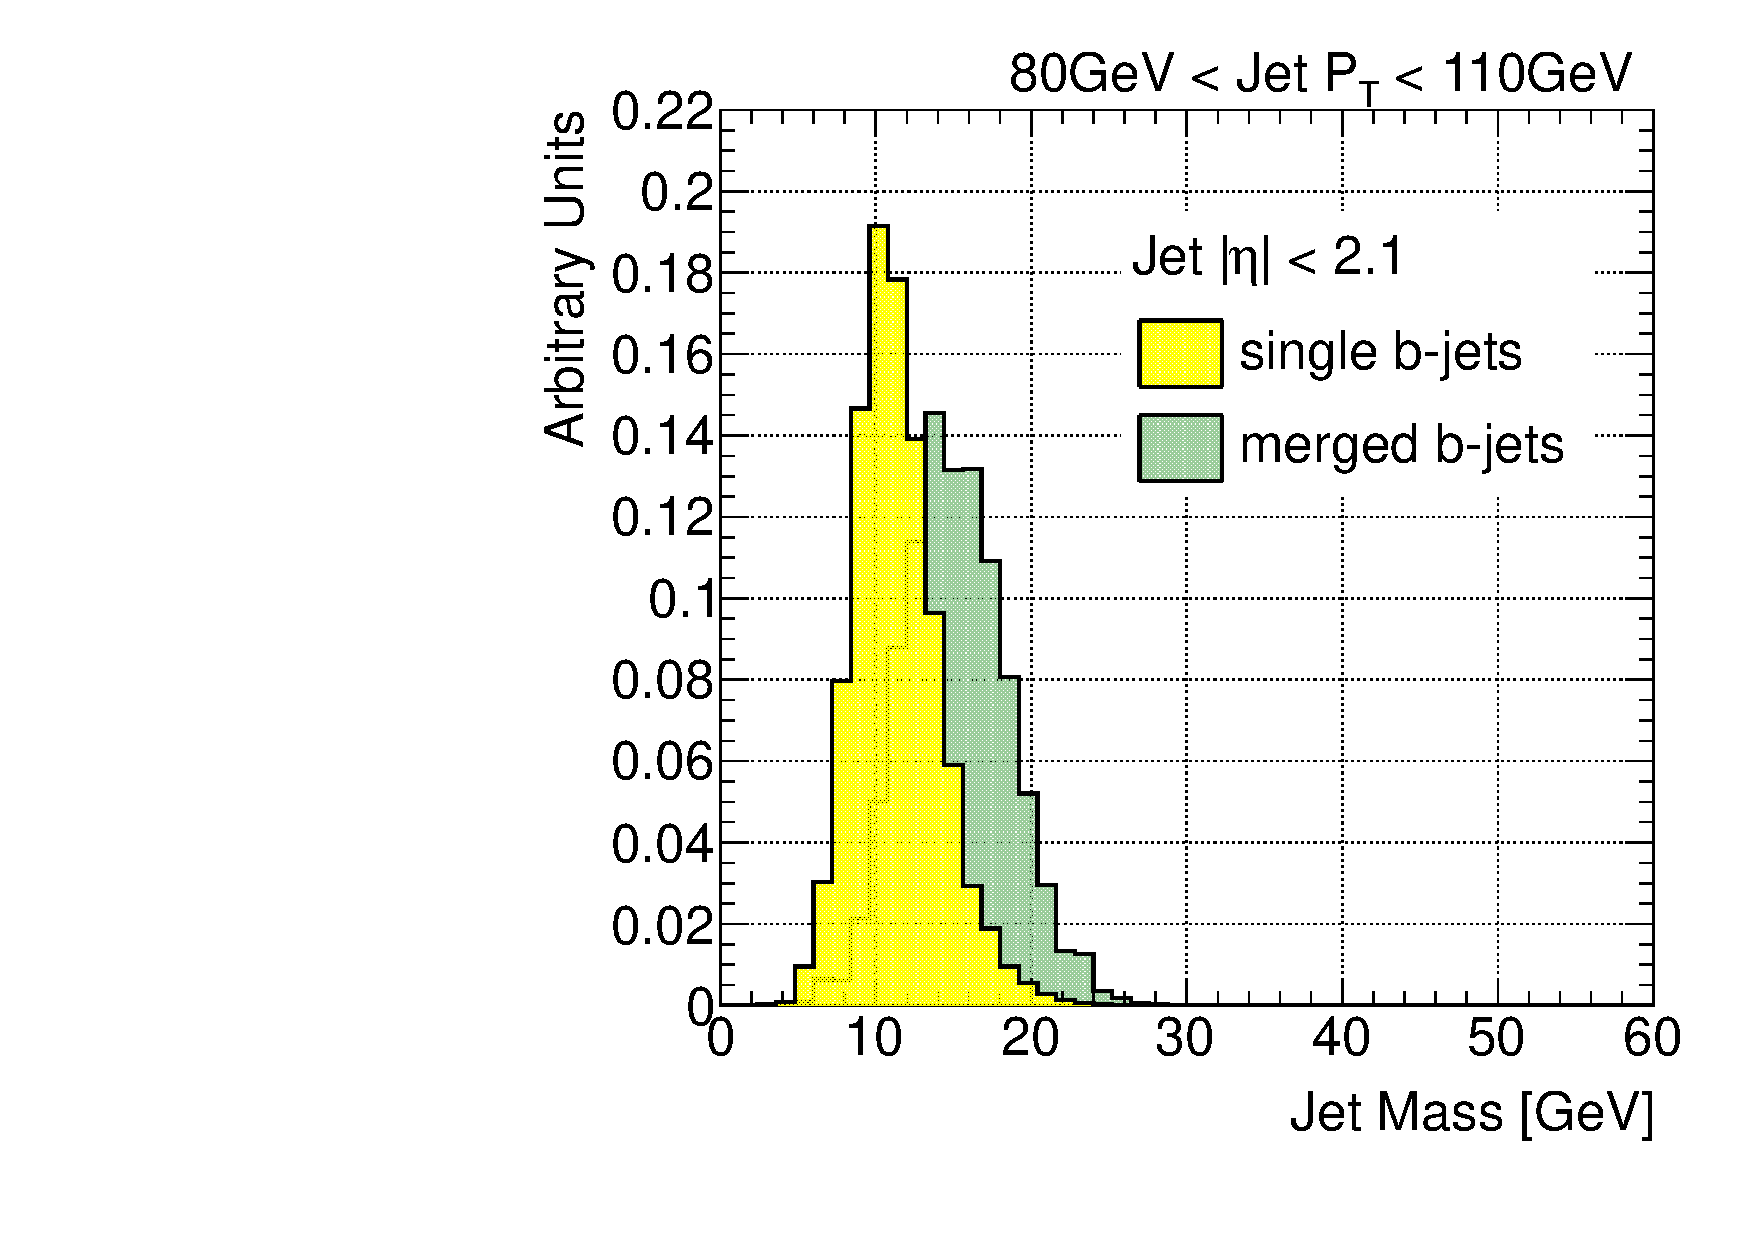
\includegraphics[width=0.49\textwidth]{FIGS/VarsSingleMerged/JetMass080.pdf}
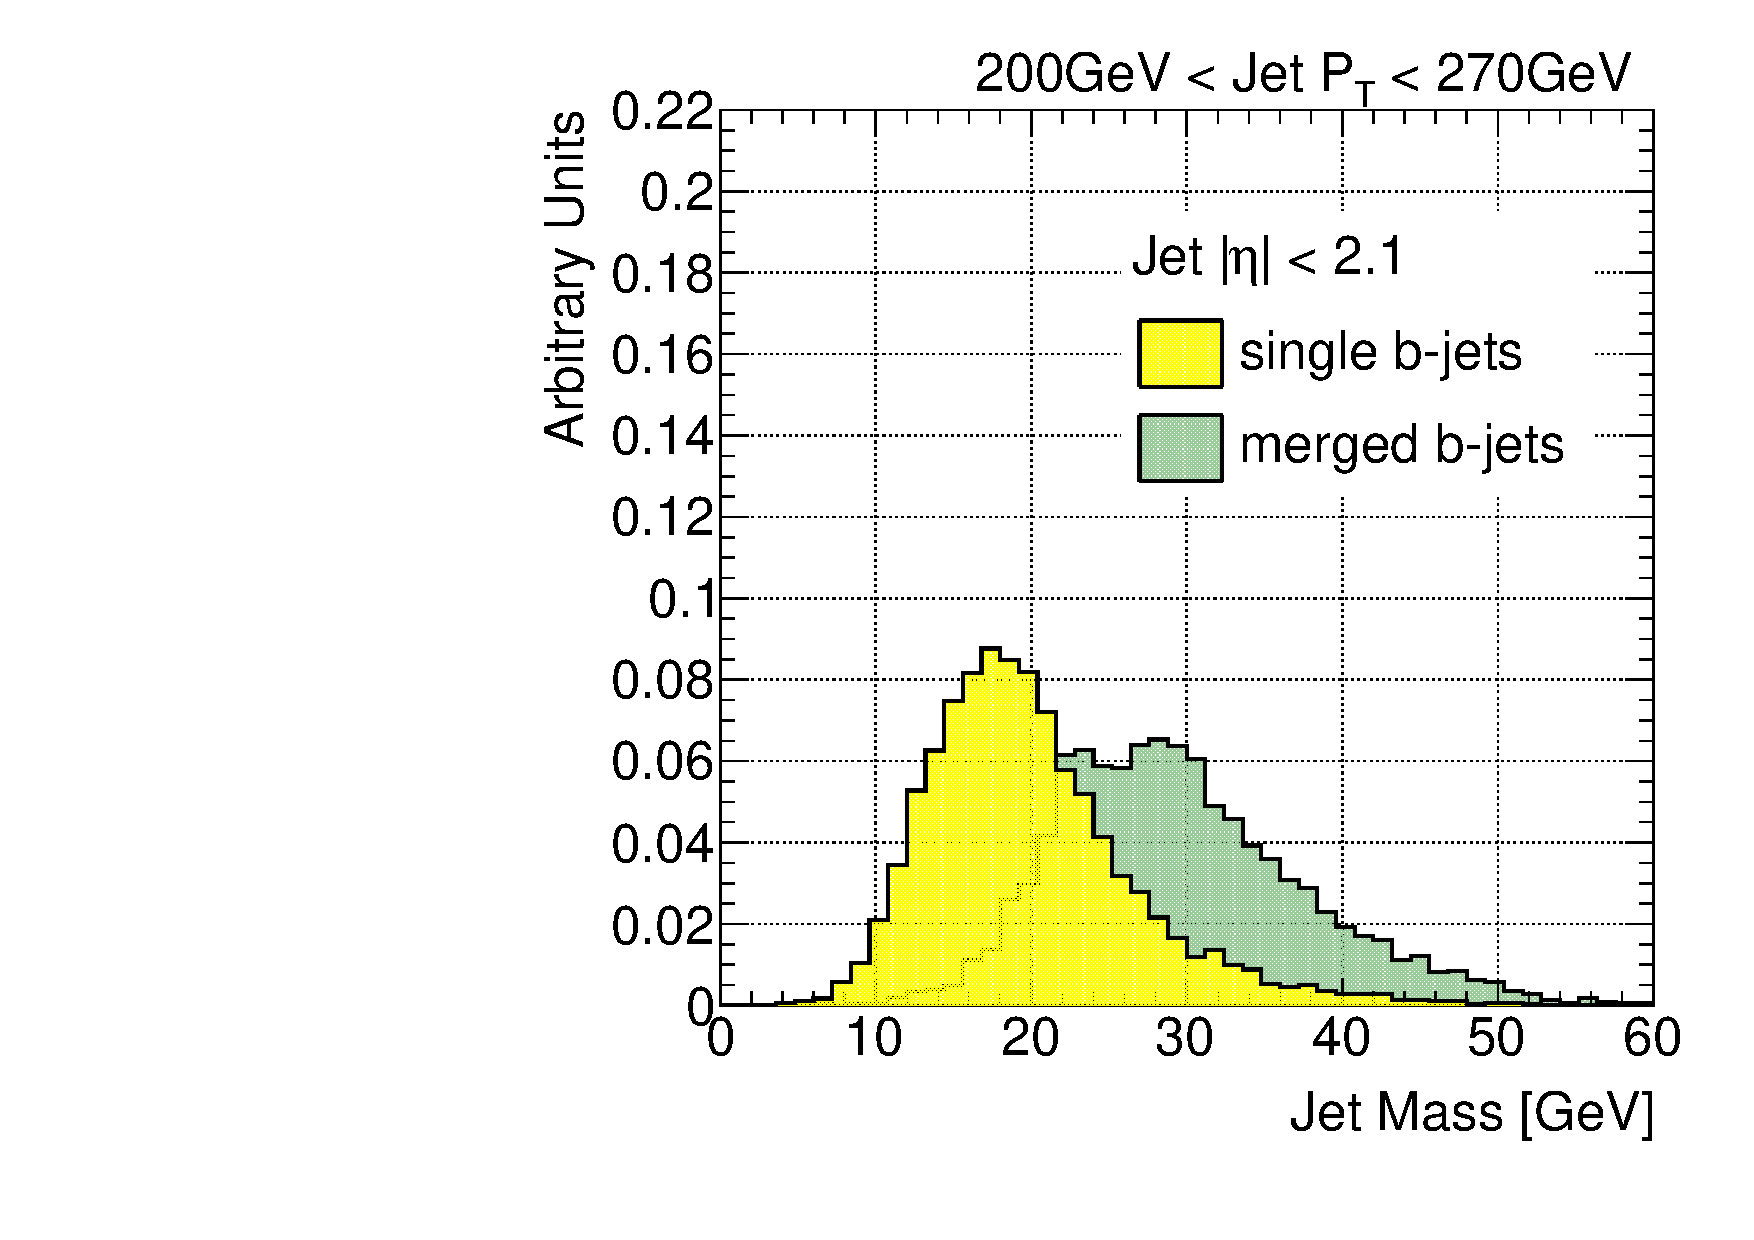
\includegraphics[width=0.49\textwidth]{FIGS/VarsSingleMerged/JetMass200.pdf}
\caption{Distribution of jet mass in~GeV for single and merged $b$-jets between 80~GeV to 110~GeV (left) and 200~GeV to 270~GeV (right).}
\label{fig:masssinglemerged}
\end{figure}


%%%%%%%%%%%%%%%%%%%%%%%%%%%%%%%%%%%%%%%%%%%%%%%%%%%%%%%%%%%%%%%%%%%%%%%%%%%%%%%%%%%%%%%%%%%%%%
%{ \em IV. $\Delta R$ between leading tracks}
%\vspace{3 mm}
{ \em $\Delta R$ between leading tracks} An alternative approach to measuring the width is to use the angular separation of the two hardest constituents inside jets. This has the advantage of removing any dependence on the shower development within the calorimeter and focuses on the hard components of the jet. Figure~\ref{fig:drtrk12singlemerged} shows the distribution of the $\Delta R$ between leading tracks in the jet for single and merged $b$-jets. The merged $b$-jet distributions are slightly broader than single $b$-jet distributions for medium $\pt$. The effect diminishes as we go to higher transverse momentum values, offering very poor discrimination.
%\vspace{3 mm}

\begin{figure}[tp]
\centering
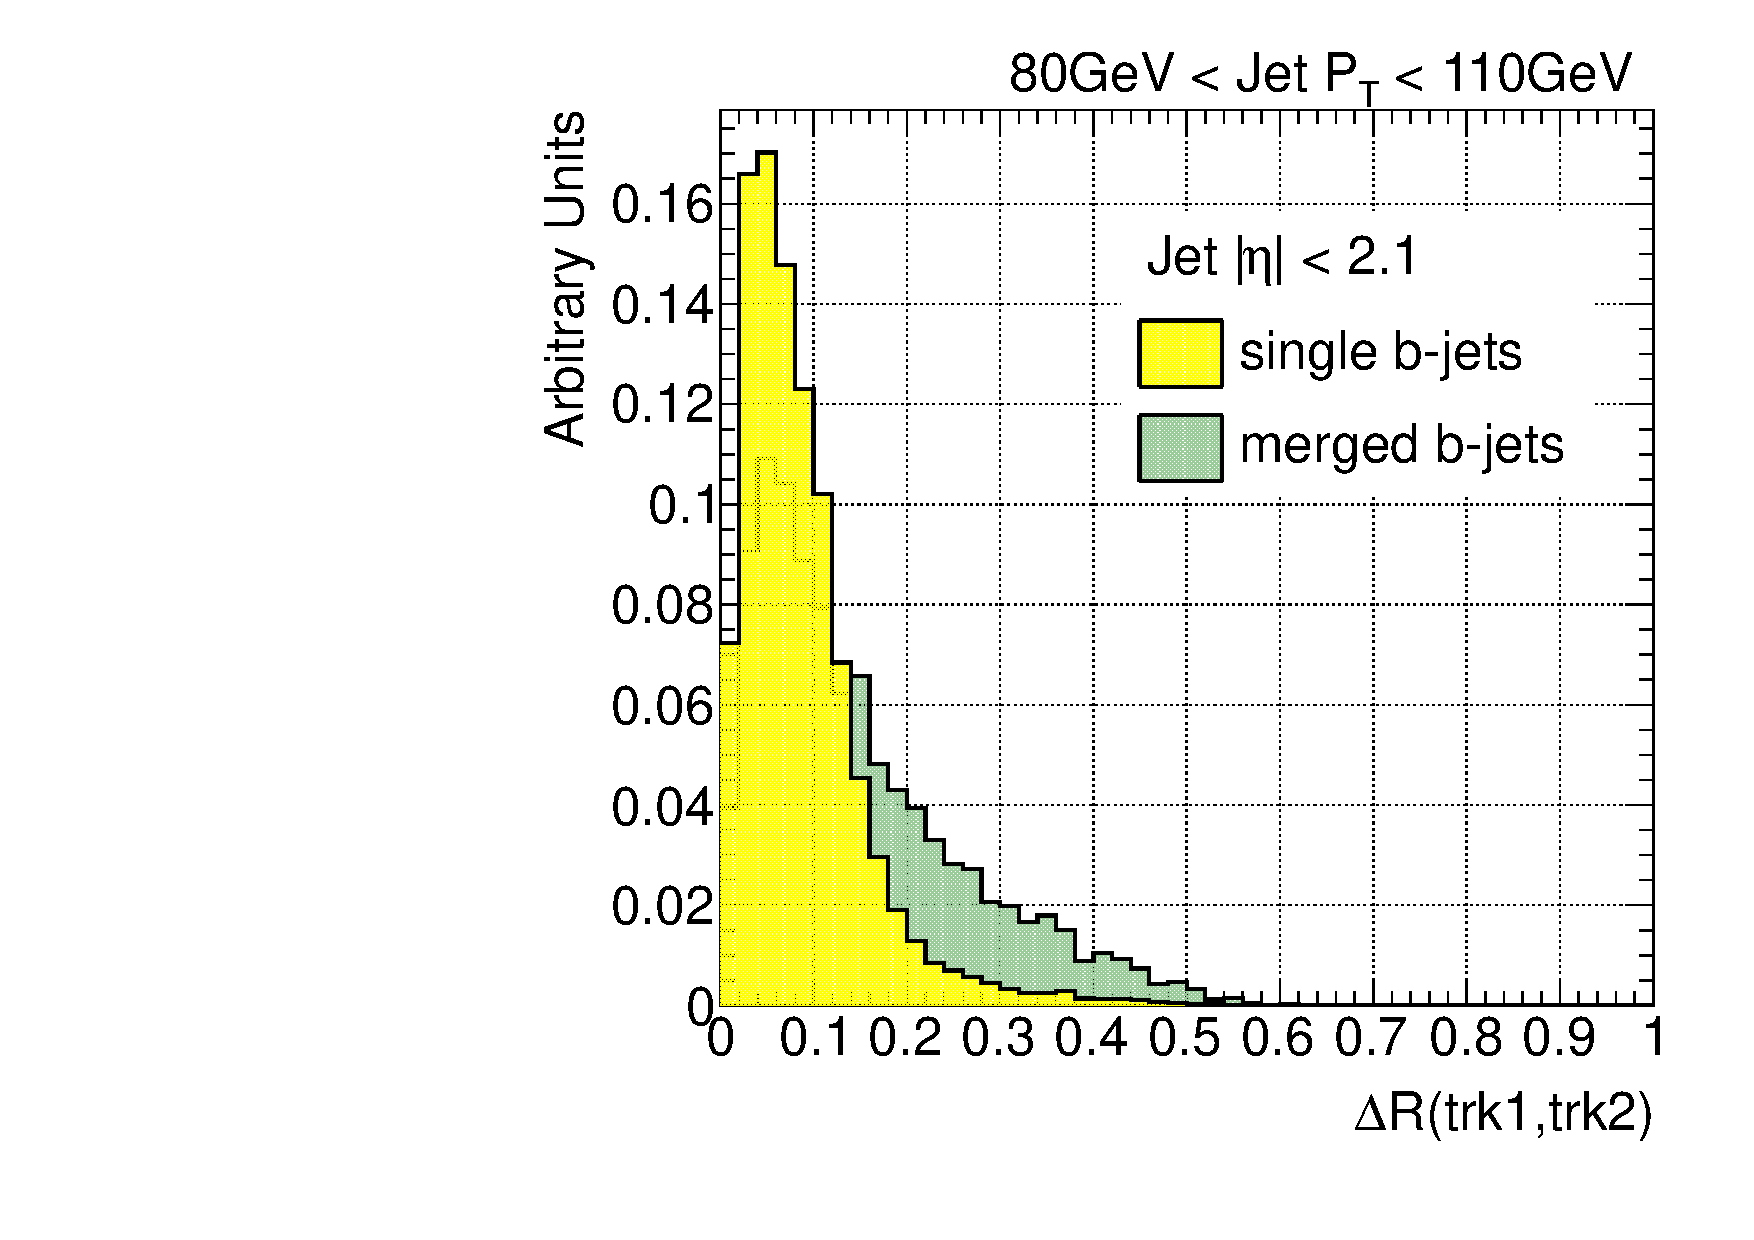
\includegraphics[width=0.49\textwidth]{FIGS/VarsSingleMerged/DRtrk12080.pdf}
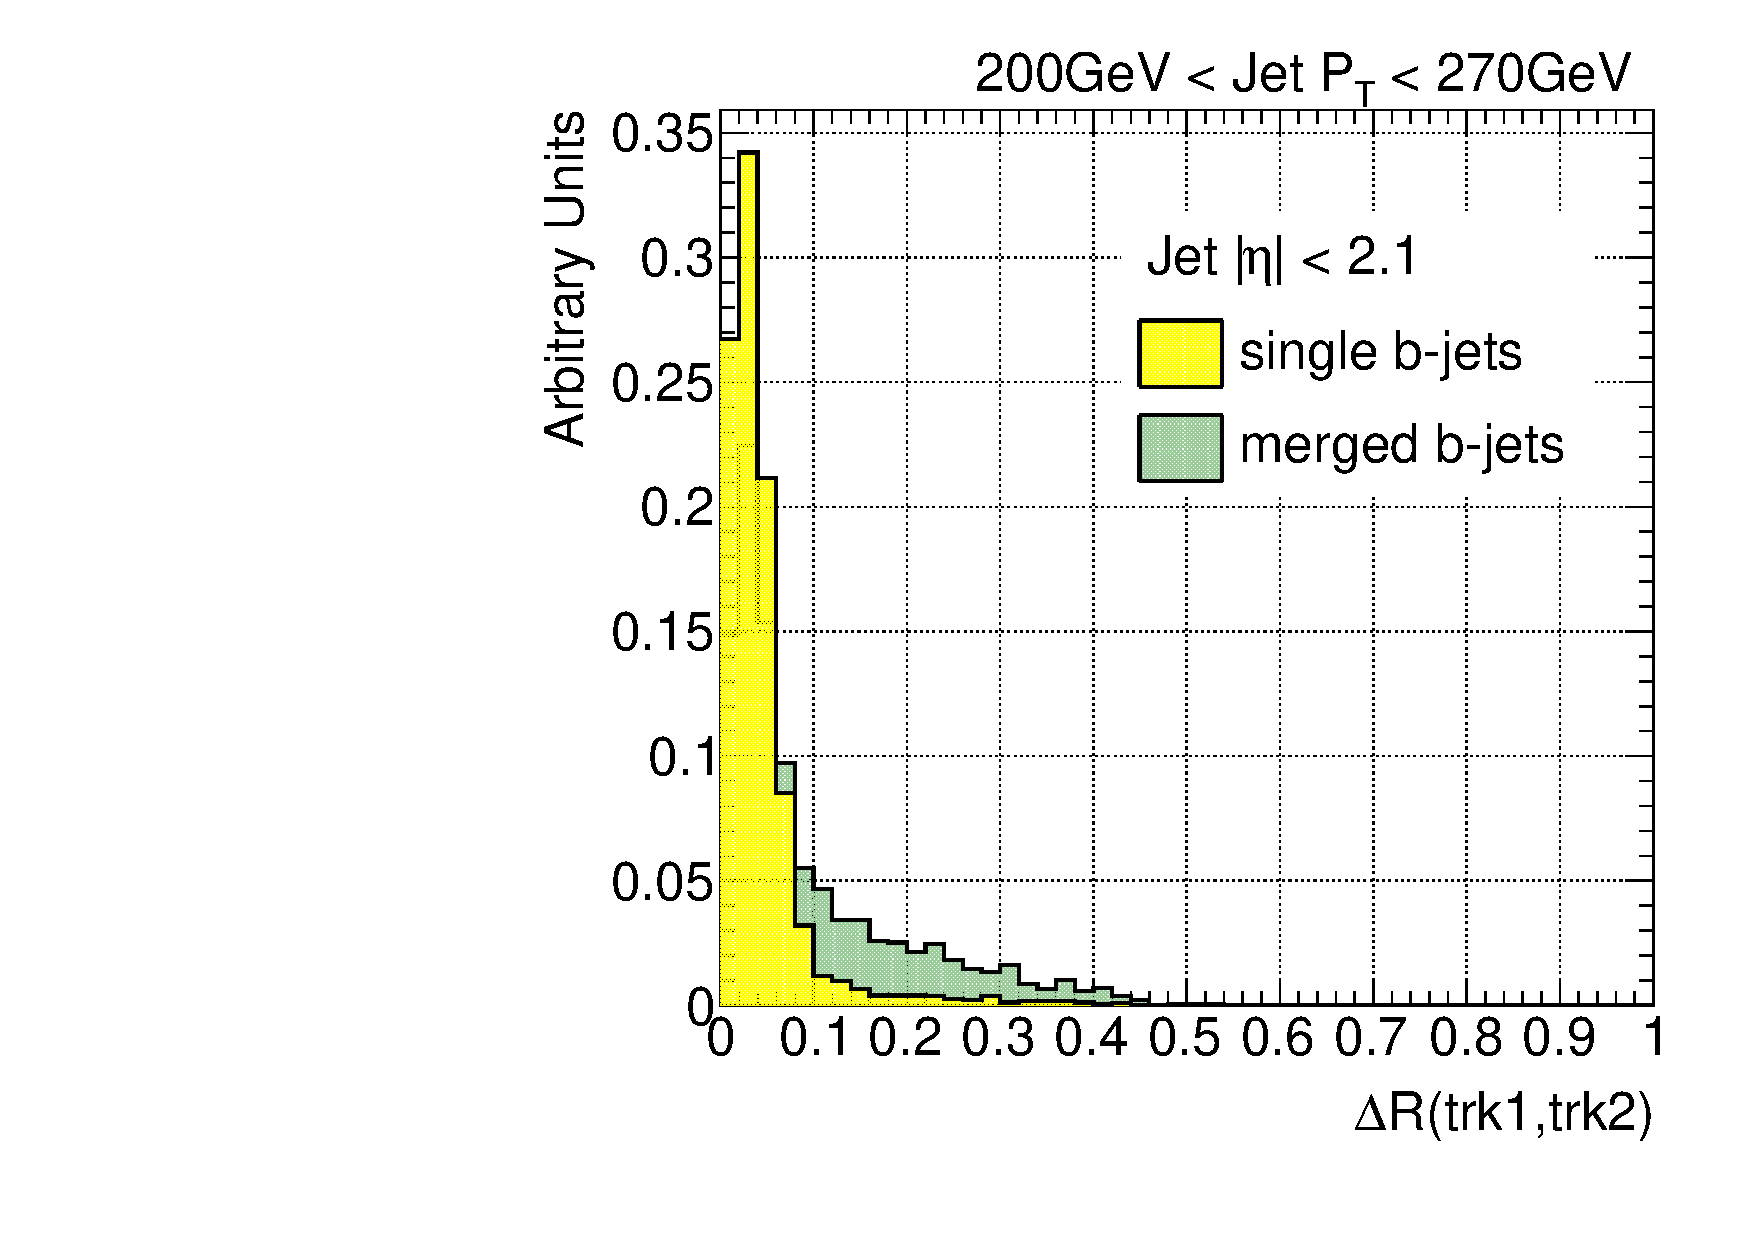
\includegraphics[width=0.49\textwidth]{FIGS/VarsSingleMerged/DRtrk12200.pdf}
\caption{Distribution of $\Delta R$ between leading tracks for single and merged $b$-jets between 80~GeV to 110~GeV (left) and 200~GeV to 270~GeV (right).}
\label{fig:drtrk12singlemerged}
\end{figure}

%%%%%%%%%%%%%%%%%%%%%%%%%%%%%%%%%%%%%%%%%%%%%%%%%%%%%%%%%%%%%%%%%%%%%%%%%%%%%%%%%%%%%%%%%%%%%%
%{ \em V. Maximum $\Delta R$ between track pairs}
%\vspace{3 mm}
{ \em Maximum $\Delta R$ between track pairs} Several other variables, besides the jet width, were investigated to expose the expected two-subjet substructure of merged $b$-jets.  The maximum $\Delta R$ separation between pairs of tracks associated to the jet ($\max\{\Delta R(trk,trk)\}$) was also evaluated as a discrimanting variable. Its distribution is shown in Fig.~\ref{fig:drmaxsinglemerged}, for single and double $b$-hadron jets. The latter shows significantly higher values for this variable over a broad range of jet $\pt$. The distinct characteristic of this variable is that the separation between single $b$-jets and merged does not depend on jet $\pt$. In spite of its good discrimination power, alternative characterising variables are desirable as $\max\{\Delta R(trk,trk)\}$ is sensitive to soft tracks originating from pile-up. 
%\vspace{3 mm}
\begin{figure}[tp]
\centering
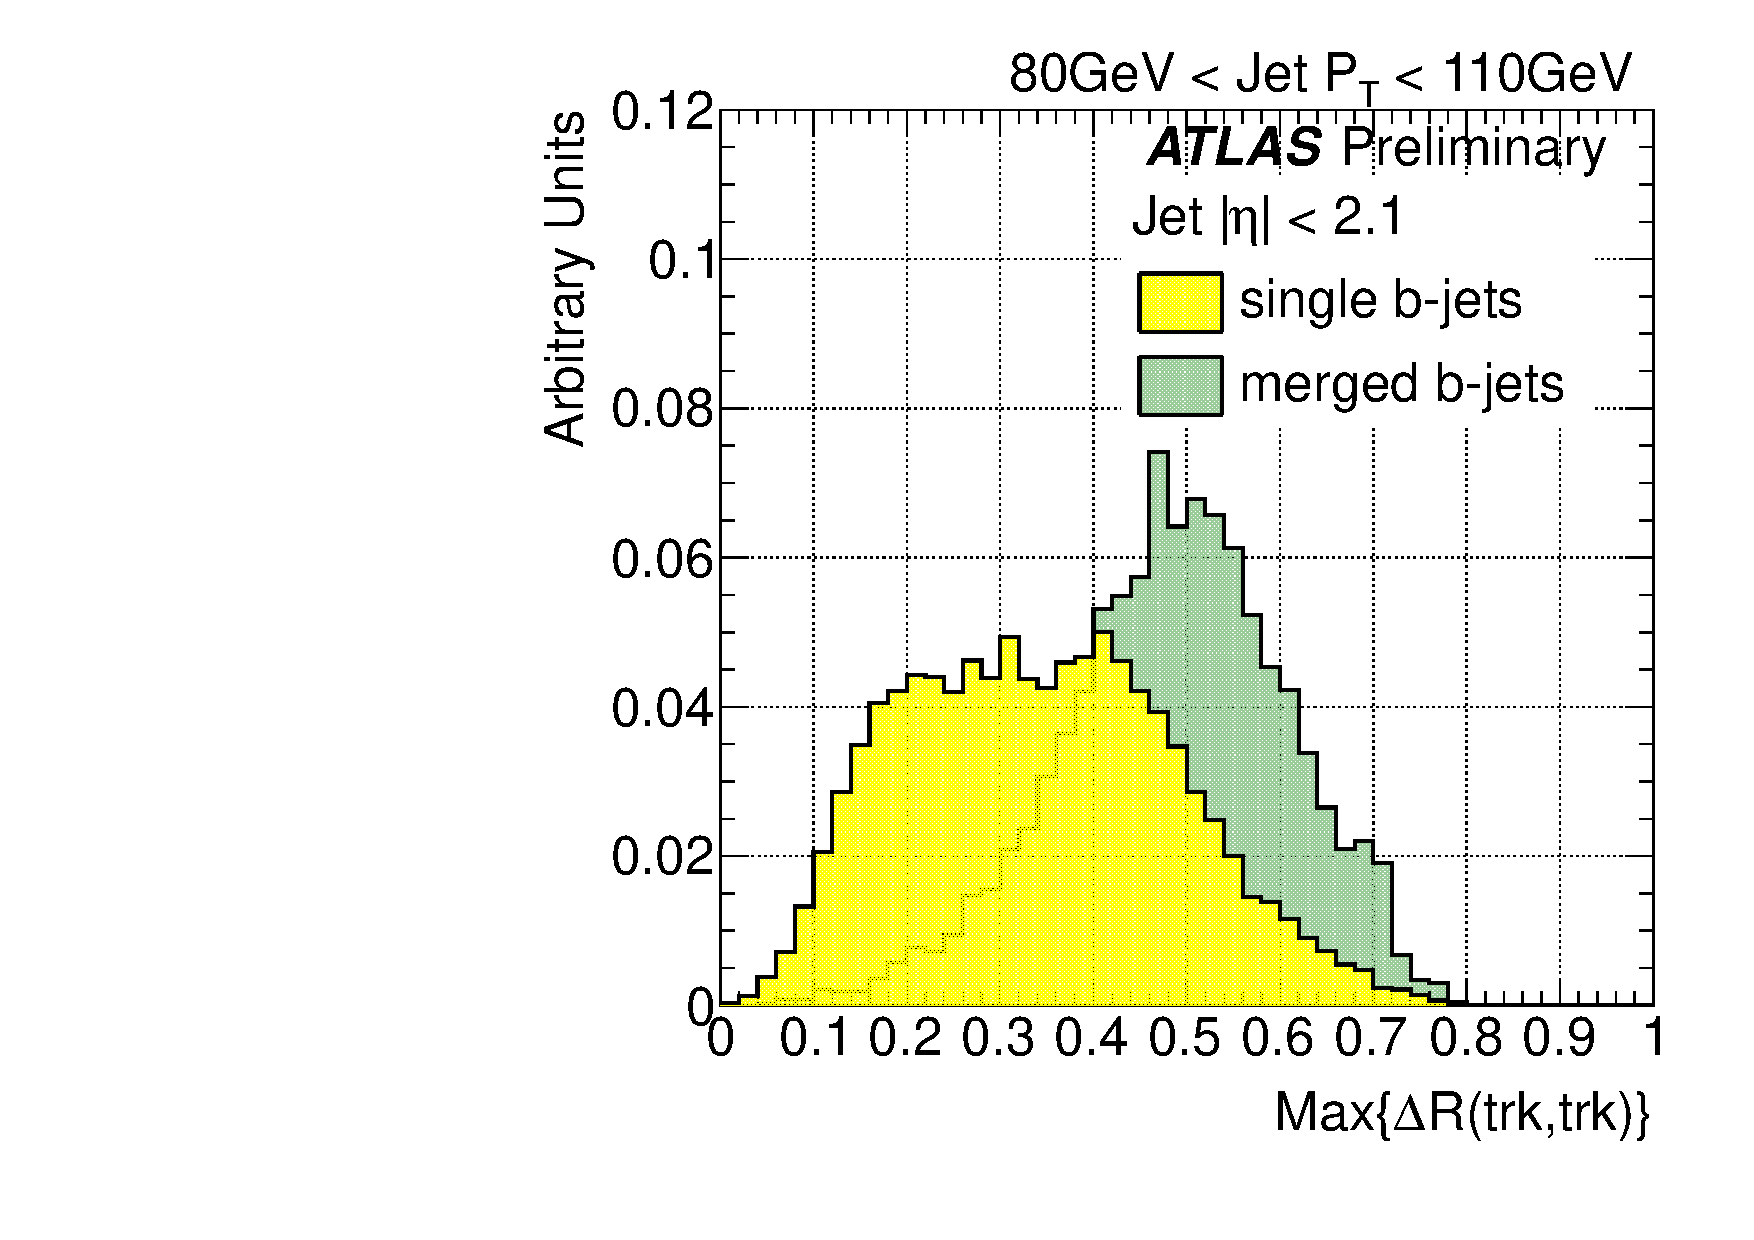
\includegraphics[width=0.49\textwidth]{FIGS/VarsSingleMerged/drmax080.pdf}
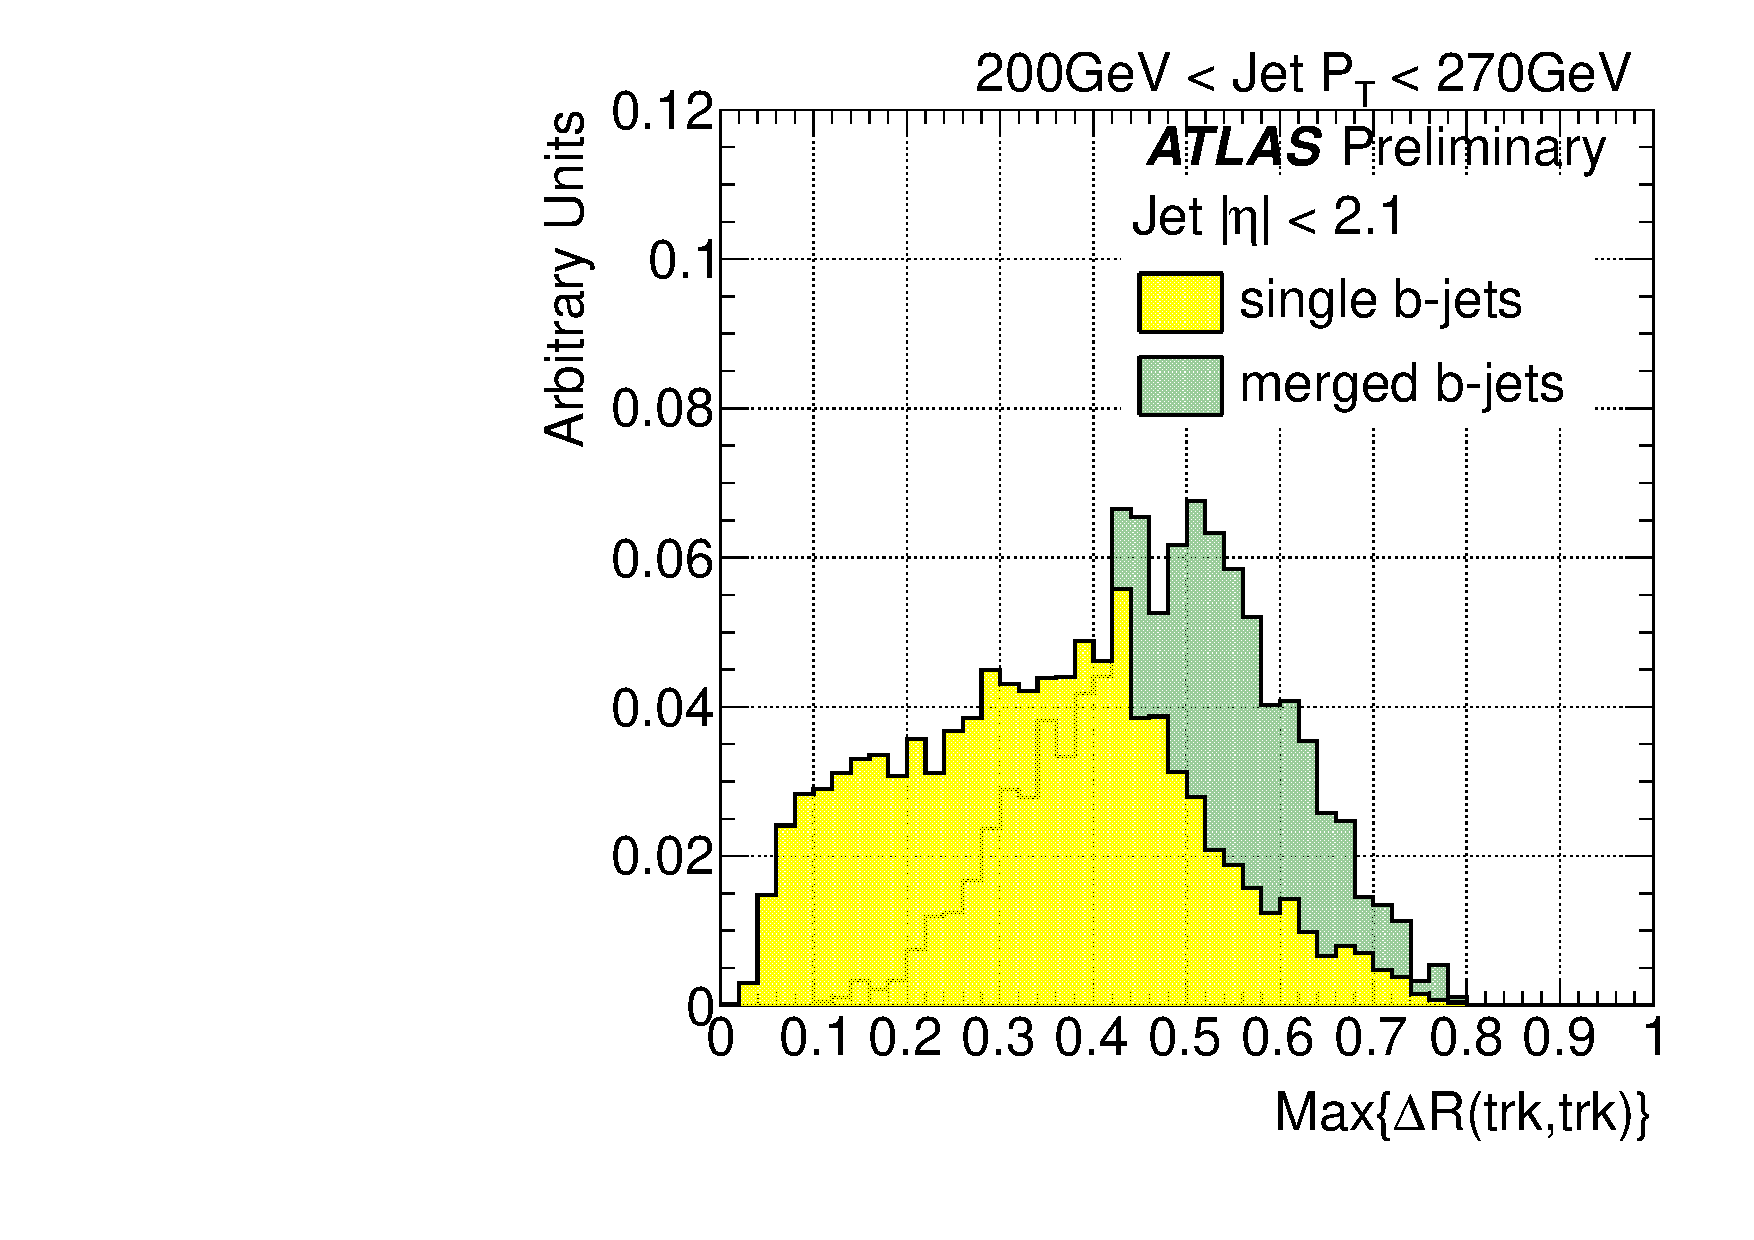
\includegraphics[width=0.49\textwidth]{FIGS/VarsSingleMerged/drmax200.pdf}
\caption{Distribution of the maximum $\Delta R$ between pairs of tracks in jets for single and merged $b$-jets between 80~GeV to 110~GeV (left) and 200~GeV to 270~GeV (right).}
\label{fig:drmaxsinglemerged}
\end{figure}


%%%%%%%%%%%%%%%%%%%%%%%%%%%%%%%%%%%%%%%%%%%%%%%%%%%%%%%%%%%%%%%%%%%%%%%%%%%%%%%%%%%%%%%%%%%%%%
%{ \em VI. Number of $k_t$ subjets}
%\vspace{3 mm}
%With the development of the $k_t$ algorithm, subjets were first used in the description of the hadronic final state in $e^+e^-$ annihilation, such as the study of the jet multiplicity at different energy scales~\cite{Catani1992445}. 

{ \em Number of $k_t$ subjets} The subjet multiplicity $-$ the number of subjets within a jet $-$ provides information on the distribution of energy and multiplicity of particles within a jet. For instance, in~\cite{Snihur1999494} the result of meassuring this variable on quark- and gluon-initiated jets indicates that gluon-initiated jets tend to have on average higher subjet multiplicity. This result is consistent with the QCD prediction that gluons radiate more than quarks. In the case of this and different other analyses % see for instance  http://iopscience.iop.org/1126-6708/1999/09/009/
the $k_t$ algorithm is rerun for subjet finding.

By using the sequential recombination algorithms introduced in Section~\ref{sec:jetalgos}, it is straightforward to define a ``subjet algorithm'' in which the structure of the jet's constituents is resolved using either the same jet finder algorithm as used for jet reconstruction or a new one with a fixed (smaller) distance parameter. 
As an alternative to fixed distance parameter subjets, it is also possible to undo the last step in the recombination sequence~\cite{kt2} in order to identify the decay products of an object.  This approach is used in seveal jet grooming procedures\footnote{Jet grooming comprises dedicated techniques to remove uncorrelated radiation within a jet. A review of these procedures can be found in~\cite{Abdesselam:2010pt}. }, see for instance~\cite{pruning}.

%In contrast to the $k_t$ algorithm, it is not useful just to undo the last stage of C/A clustering: The absence of any momentum scale in its distance measure means that the last clustering often involves soft radiation on the edges of the jet and so, is unrelated to the heavy object's decay. 
%The so-called BDRS method of jet grooming
%http://prl.aps.org/abstract/PRL/v100/i24/e242001
% uses the C/A algorithm. Subjets are then defined by de-clustering the C/A algorithm and evaluating the relative mass of the subjets compared to the parent jet. As a final step, the three hardest identified subjets are recombined to define the resulting ``filtered'' jet.

Figure~\ref{fig:nsubjetsinglemerged} shows the distribution of the number of subjets for single and merged $b$-jets. The subjets in this case were built using the associated tracks as constituents, clustered by the inclusive $k_t$ algorithm with distance parameter $R=0.2$. The discrimination power of this variable, as it is defined, turned out to be very poor.
%\vspace{3 mm}

\begin{figure}[tp]
\centering
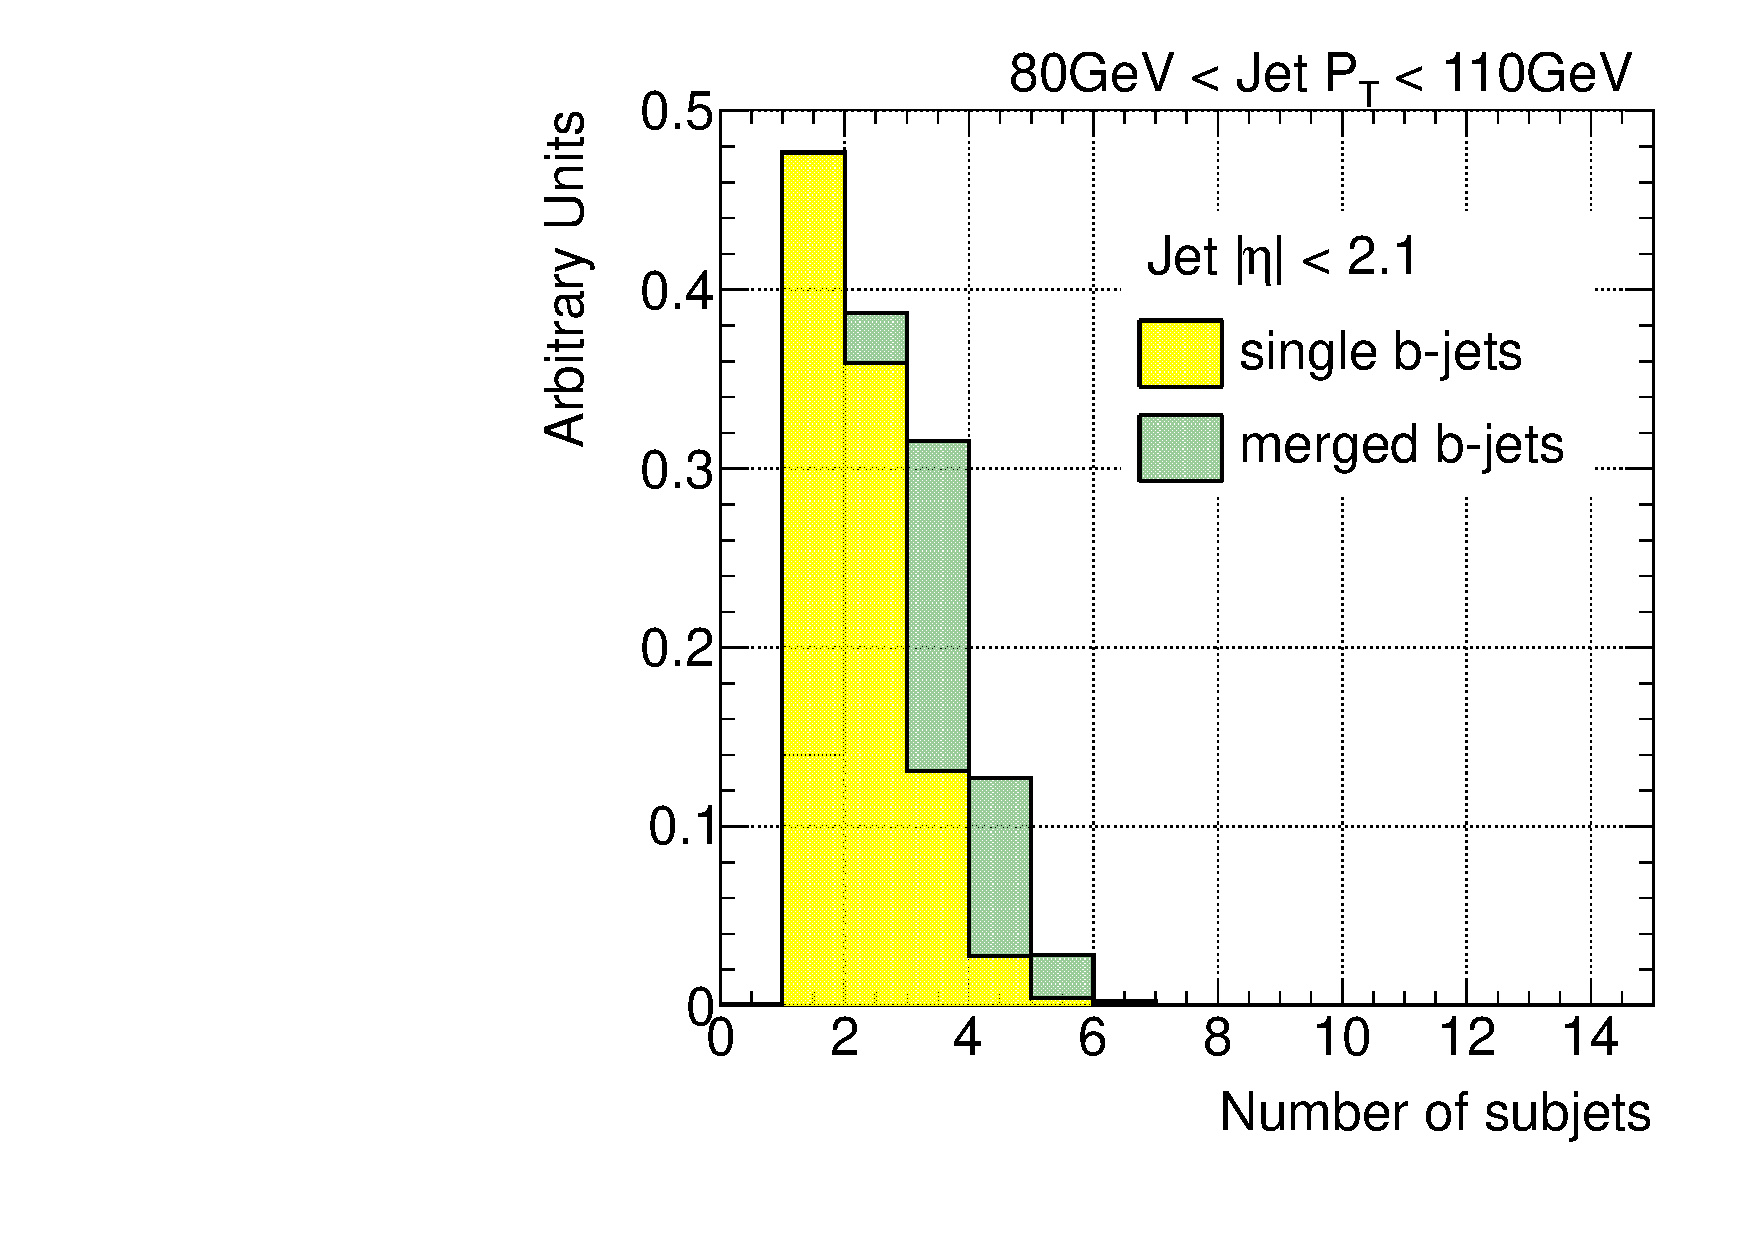
\includegraphics[width=0.49\textwidth]{FIGS/VarsSingleMerged/Nsubjets080.pdf}
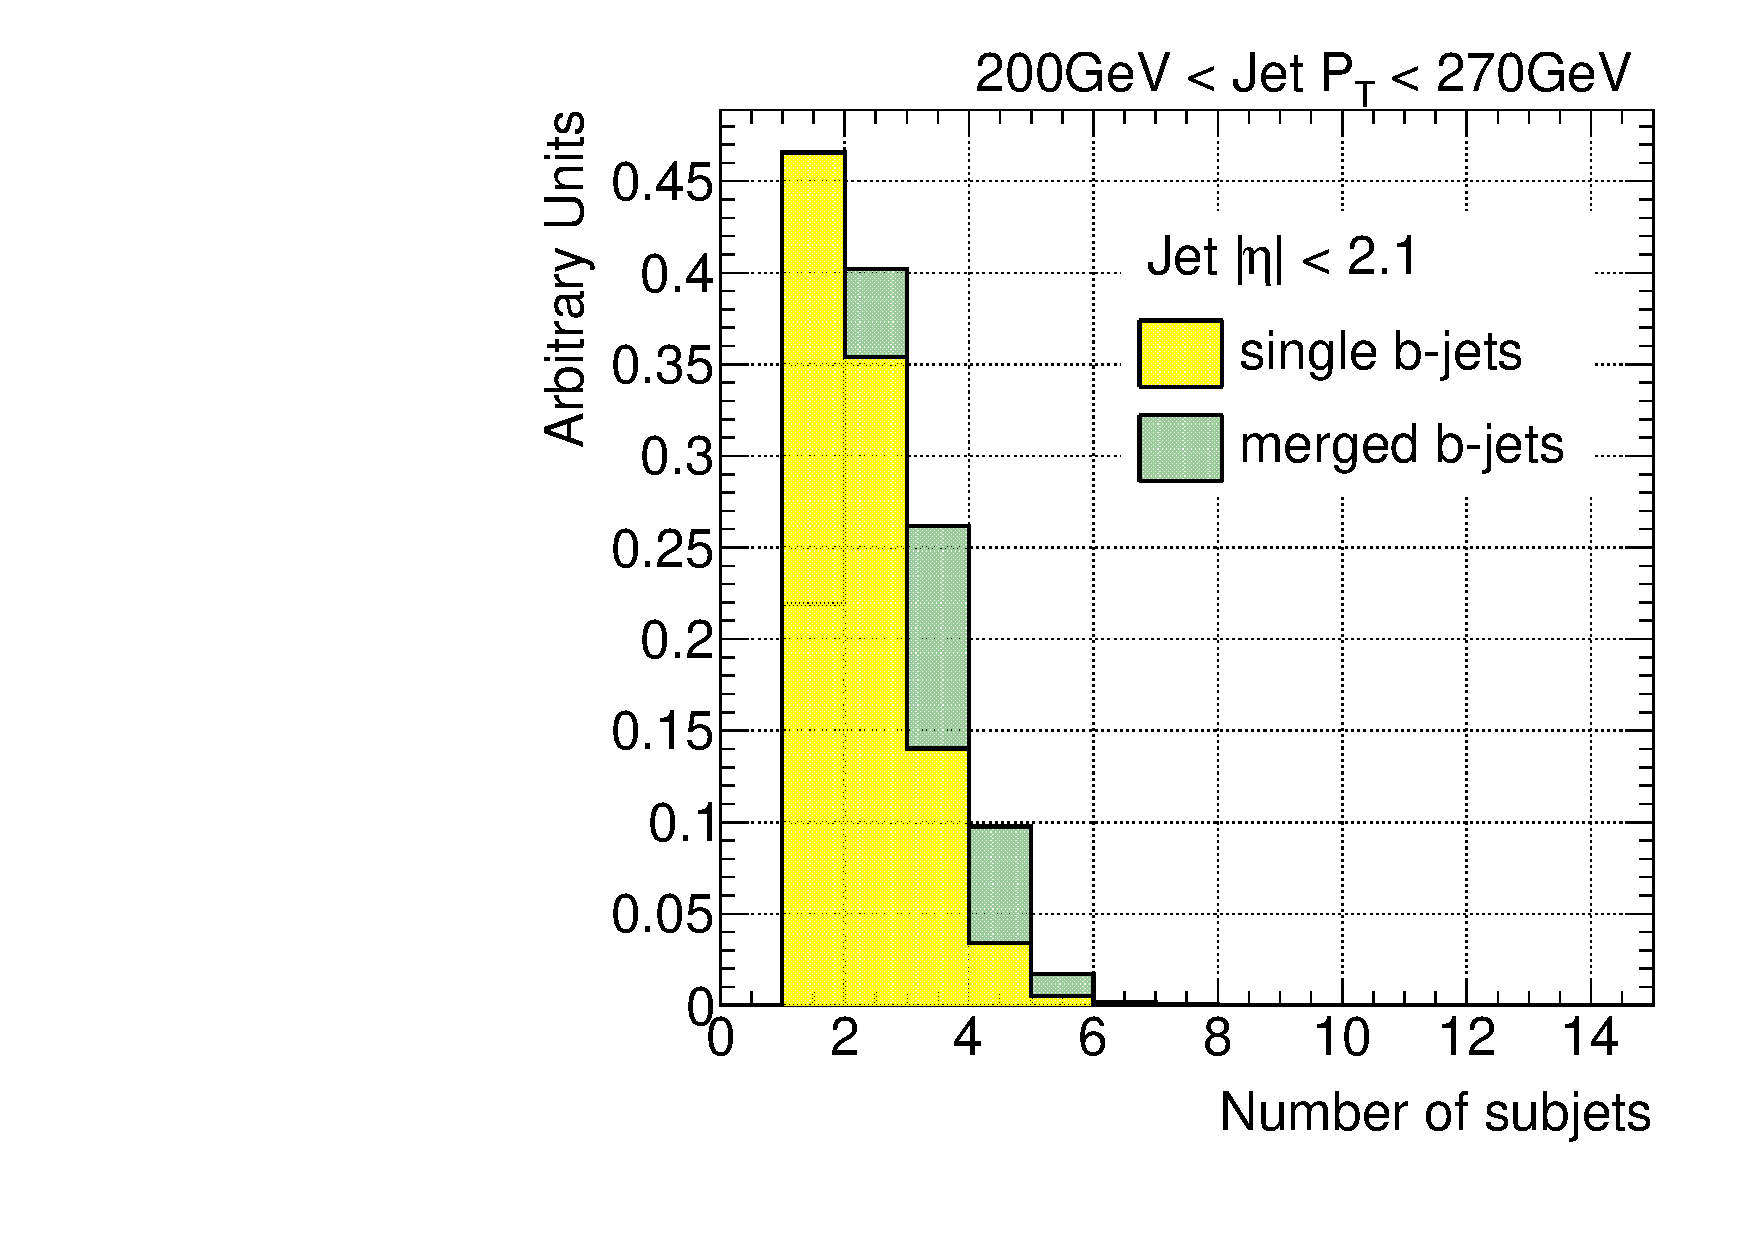
\includegraphics[width=0.49\textwidth]{FIGS/VarsSingleMerged/Nsubjets200.pdf}
\caption{Distribution of the number of $k_t$ sub-track-jets for single and merged $b$-jets between 80~GeV to 110~GeV (left) and 200~GeV to 270~GeV (right).}
\label{fig:nsubjetsinglemerged}
\end{figure}


%%%%%%%%%%%%%%%%%%%%%%%%%%%%%%%%%%%%%%%%%%%%%%%%%%%%%%%%%%%%%%%%%%%%%%%%%%%%%%%%%%%%%%%%%%%%%%%%%%
%{ \em VII. $\Delta R$ between the axes of two $k_t$ subjets}
%\vspace{3 mm}

{ \em $\Delta R$ between the axes of two $k_t$ subjets}  The $\Delta R$ between $k_t$ subjets is obtained by applying the exclusive $k_t$ algorithm~\cite{exclusivekt} to the tracks associated to the jet using a large $k_t$ distance parameter to ensure that all tracks get combined. The clustering is stopped once it reaches exactly two jets. The $\Delta R$ between the axes of the two exclusive subjets is shown in Fig.~\ref{fig:drktsinglemerged}.  As expected, it is larger for merged than for single jets. We observe that this
variable provides very good separation, with the advantage of infrared safety and insensitivity to pile-up as opposed to $\max\{\Delta R((trk,trk)\}$.
%\vspace{3 mm}

\begin{figure}[tp]
\centering
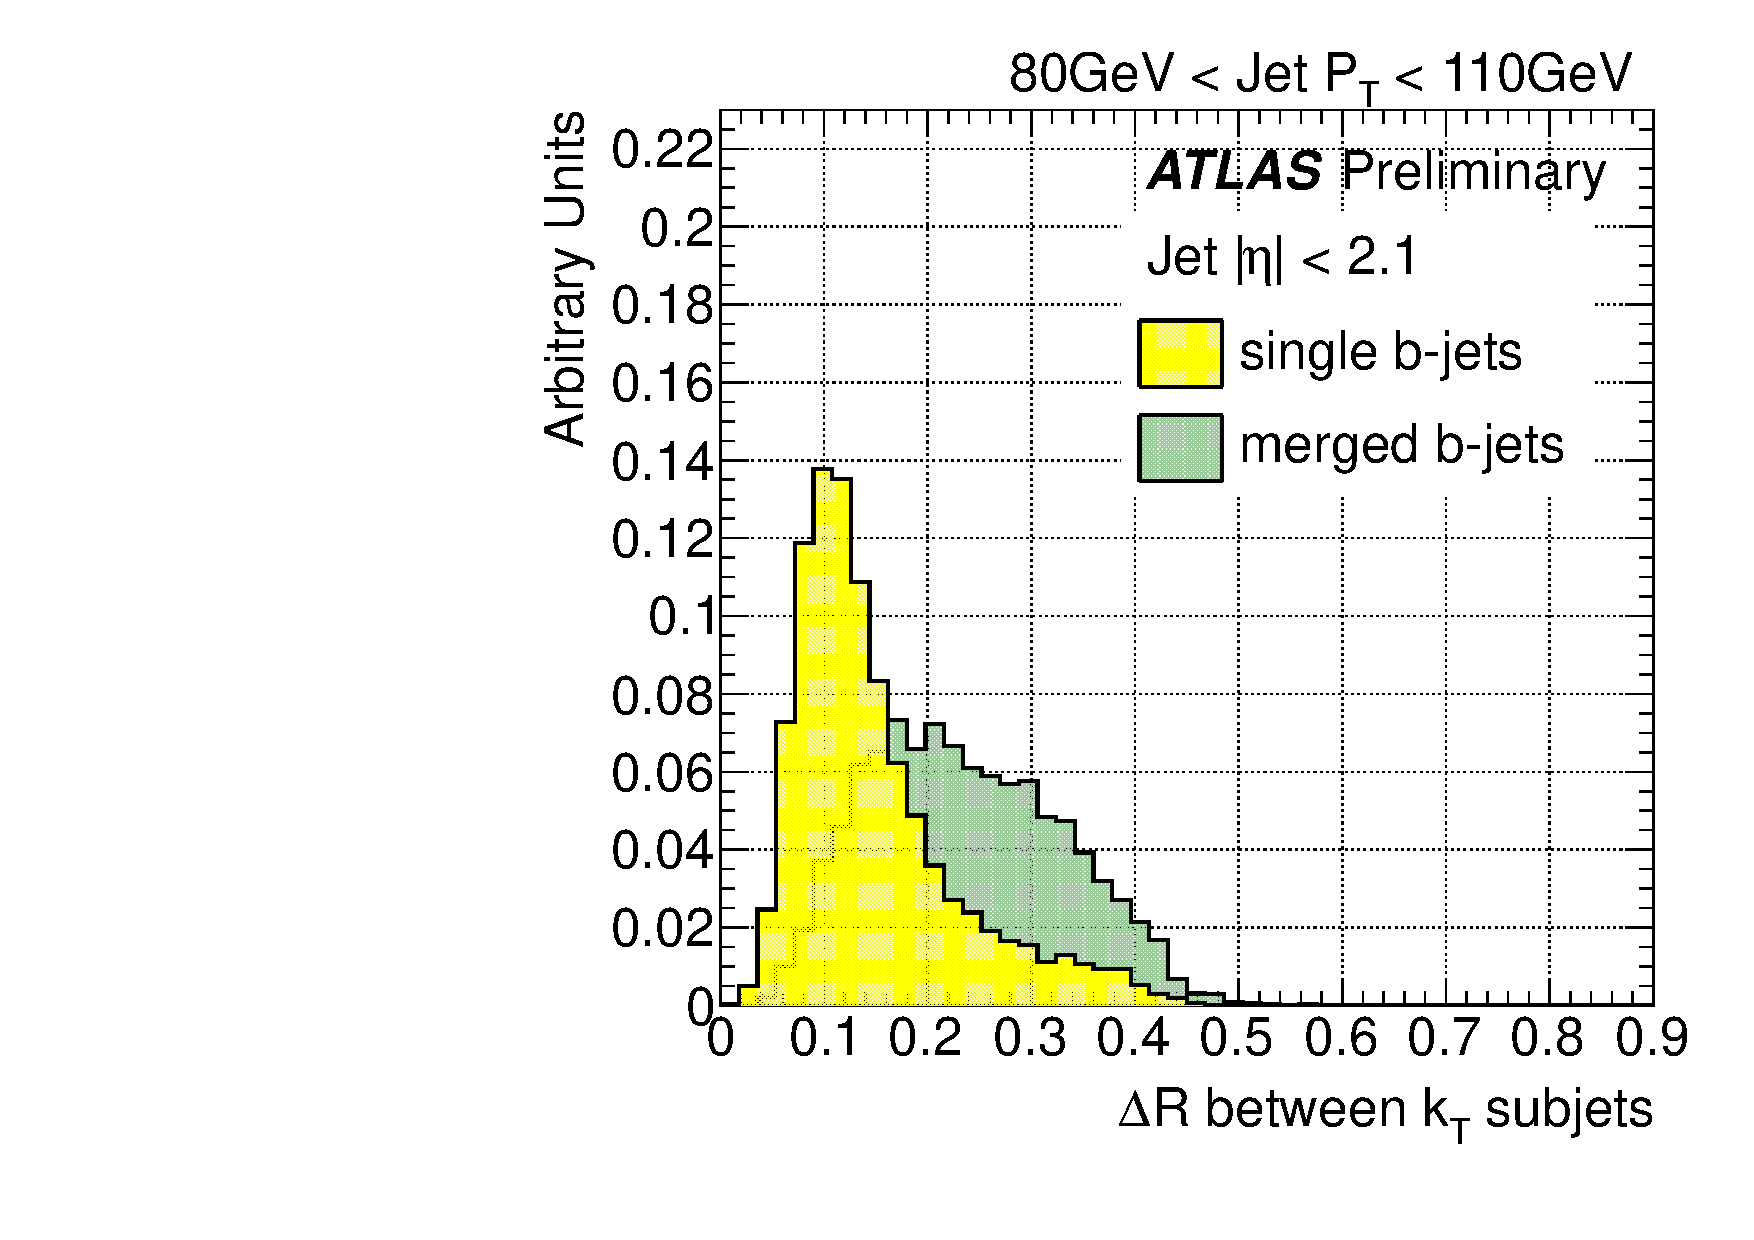
\includegraphics[width=0.49\textwidth]{FIGS/VarsSingleMerged/DRkt2axes080.pdf}
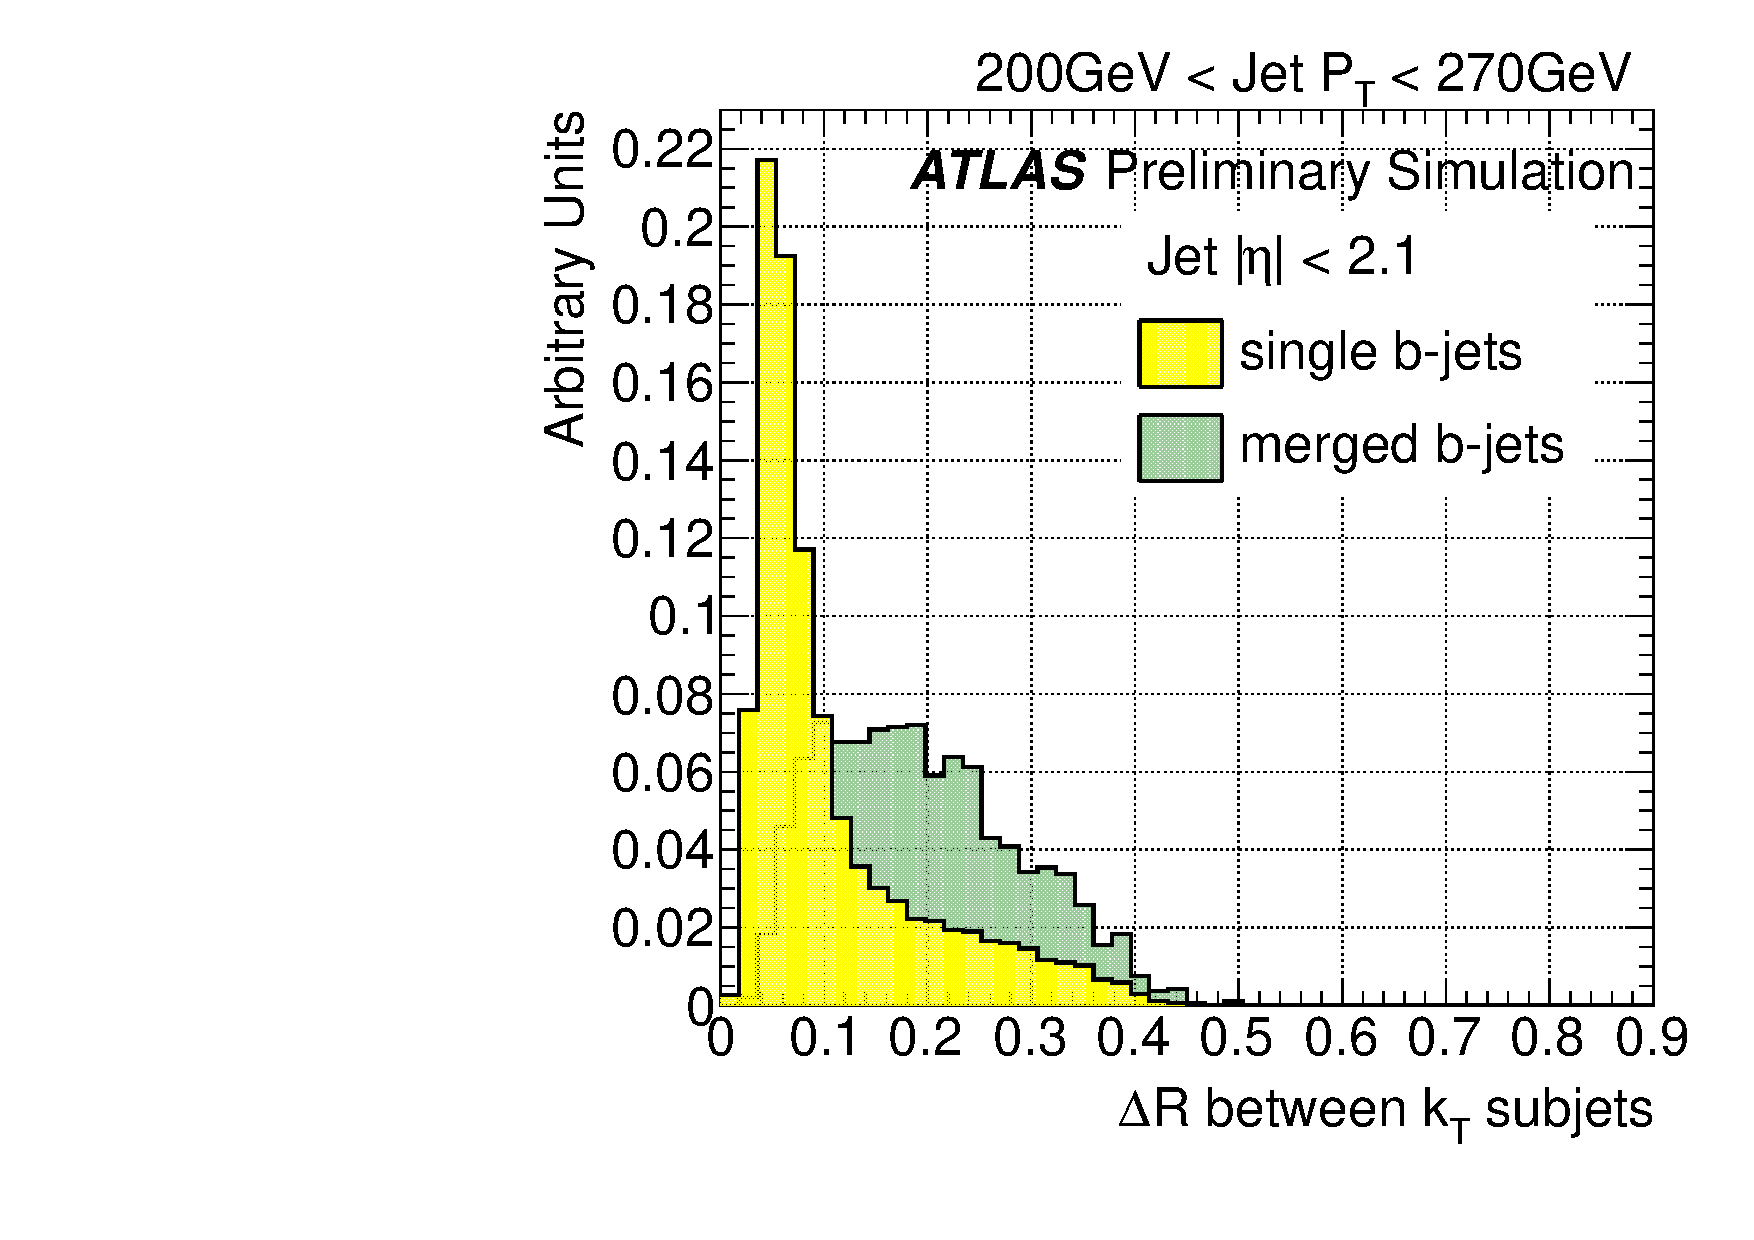
\includegraphics[width=0.49\textwidth]{FIGS/VarsSingleMerged/DRkt2axes200.pdf}
\caption{Distribution of the $\Delta R$ between the axes of the two $k_t$ subjets in the jet for single and merged $b$-jets between 80~GeV to 110~GeV (left) and 200~GeV to 270~GeV (right).}
\label{fig:drktsinglemerged}
\end{figure}

% El plot de DeltaRkt para B-trackjets vs. track-jets explica la cola que ustedes veian para b-jets y que no entendiamos. Viene de la gluon radiation! cuando uno calcula DRkt con B-tracks, la cola se reduce significativamente y b se separa mucho mas de bb. Muy interesante!
%http://slac.stanford.edu/~swiatlow/gbb_plots07_07/drktaxes_B_J3_PT80.png

%%%%%%%%%%%%%%%%%%%%%%%%%%%%%%%%%%%%%%%%%%%%%%%%%%%%%%%%%%%%%%%%%%%%%%%%%%%%%%%%%%%%%%%%%%%%%%%%%%
%{ \em VIII. $N$-subjettiness variables}
%\vspace{3 mm}

{ \em $N$-subjettiness variables} It is possible to extend the use of individual subjets in conjunction with more traditional jet shape variables. Using these tools, an inclusive jet shape based on the substructure topology of a single jet, ``$N$-subjettiness''~\cite{nsubjettiness} is defined. This variable describes the energy flow within a jet, quantifying the degree to which radiation is aligned along specified subjet axes. This jet shape was adapted from the event shape $N$-jettiness~\cite{njetti}.

Given candidate subjets directions determined by an external algorithm such as the exclusive $k_t$ procedure, the variable is defined as,
%
\begin{equation} 
\tau^{(\beta)}_N = \frac{1}{\sum_k {\pt}_k\,(R_0)^{\beta}} \sum_k {\pt}_k (\min \{ \Delta R_{j1,k},\,\Delta R_{j2,k},...,\,\Delta R_{jN,k} \})^{\beta}.
\label{eqn:nsubjet}
\end{equation} 
%
The sum runs over the $k$ constituent particles in a given jet where $p_{T,k}$ are their transverse momenta, and $\Delta R_{j1,k}$ is the distance between the candidate subjet $j1$ and a constituent particle $k$.  $R_0$ is the characteristic jet radius used in the original jet clustering algorithm.  The exponential weight, $\beta$, can optionally be applied to the angular distance computed between the subjets and the jet constituents.   
Since eq.~\ref{eqn:nsubjet} is linear in each of the constituent particle momenta, this variable is an infrared- and colliner-safe observable.


%This jet shape was designed to identify boosted $N$-prong hadronic decays. With $\beta=1$, the definition above indicates that jets with $\tau_N\approx 0$ have all their radiation aligned with the candidate subjet directions and therefore have $N$ (or fewer) subjets. Jets with $\tau_N\gg 0$ have a large fraction of their energy distributed away from the candidate subjet direction and therefore have at least $N+1$ subjets.
This jet shape was designed to separate boosted hadronic objects, like electroweak bosons and top quarks decaying into collimated showers of hadrons which a standard jet algorithm would reconstruct as single jets. % from the QCD jet background. %the complete set of  $\tau_N$ (with different values of $\beta$) could be used in a multivariate analysis. 
A simple cut on the ratio $\tau_N/\tau_{N-1}$ provides excellent discrimination power for $N$-prong hadronic objects\cite{nsubjettiness} . In particular, $\tau_2/\tau_1$ can identify boosted $W/Z$ and Higgs bosons, with the angular weighting exponent $\beta =1$ providing the best discrimination.

% In subsequent work~\cite{mininsubjettiness}, Thaler and van Tilburg showed that 
The definition of $N$-subjettiness is not unique, and different choises can be used to give different weights to the emissions within a jet. The initial step of choosing candidate subjet axes is in fact unnecessary; the quantity in equation~\ref{eqn:nsubjet} can be minimised over the candidate subjet directions, further improving boosted object discrimination.

%The definition of $N$-subjettiness is not unique, and different choises can be used to give different weights to the emissions within a jet. There generalizations of $N$-subjettiness are similar to different ``angularities''~\cite{angularities} used in $e^+e^- \rightarrow$ hadrons measurements.


%From Nsubjettiness paper
%use $N$-subjettiness to effectively ``count'' the number of subjets in a jet. Compare to previous jet substructure techniques, $N$-subjettiness  has the advantage of finding jets that contain two or more lobes of energy.
%Subjet candidates where determined by using the exclusive $k_t$ algorithm, forcing it to return exactly $N$ jets.

To avoid dependence on pile-up we consider track-based $n$-subjettiness, where the sum 
 is over the tracks in the $b$-tagged jet. As seen for massive boosted objects, a jet with a two pronged structure, with all tracks clustered along two directions, is expected to have a smaller $\tau_2$ value than a jet with a more uniform track distribution. The distributions of $\tau_2$, shown in Fig.~\ref{fig:tau2singlemerged}, display good separation between single and merged jets, but with the latter showing larger values than single. 
This behavior can be traced to the level of correlation between $\tau_2$ and track-jet width, displayed in Fig.~\ref{fig:tau2trkwidthsinglemerged}a, to be compared to the much lower correlation presented, for instance, between track-jet width and the jet track multiplicity, shown in  Fig.~\ref{fig:tau2trkwidthsinglemerged}b. 

The correlation observed suggests to switch from an absolute to a width-normalized $\tau_2$, and evaluate the ratio $\tau_2/\tau_1$. Fig.~\ref{fig:tauratiosinglemerged} thus shows the distributions for this observable. Somewhat larger values are obtained for single than for merged $b$-jets, specially at high $\pt$, however we decided not to use this variable as it offers only marginal discrimination. 

%In spite of its expected 2-prong substructure, merged $b$-jets have higher values of $ \tau_2$ than single $b$-jets.  The explanation of this behavior can be found in Fig.~\ref{fig:tau2trkwidthsinglemerged}, where its correlation with  track-jet width ($\sim \tau_1$) is shown for single and merged $b$-jets. The two variables are highly correlated and for this reason wider jets  have a larger $ \tau_2$. This suggests to switch from an absolute to a width-normalized$\tau_2$. Fig.~\ref{fig:tauratiosinglemerged} thus shows the distributions of $\tau_2/\tau_1$. This ratio is often used but, although as expected somewhat larger values are obtained for single than for merged $b$-jets, specially at high $\pt$, we decided not to use this variable as it offers only marginal discrimination. 
%\vspace{3 mm}

\begin{figure}[tp]
\centering
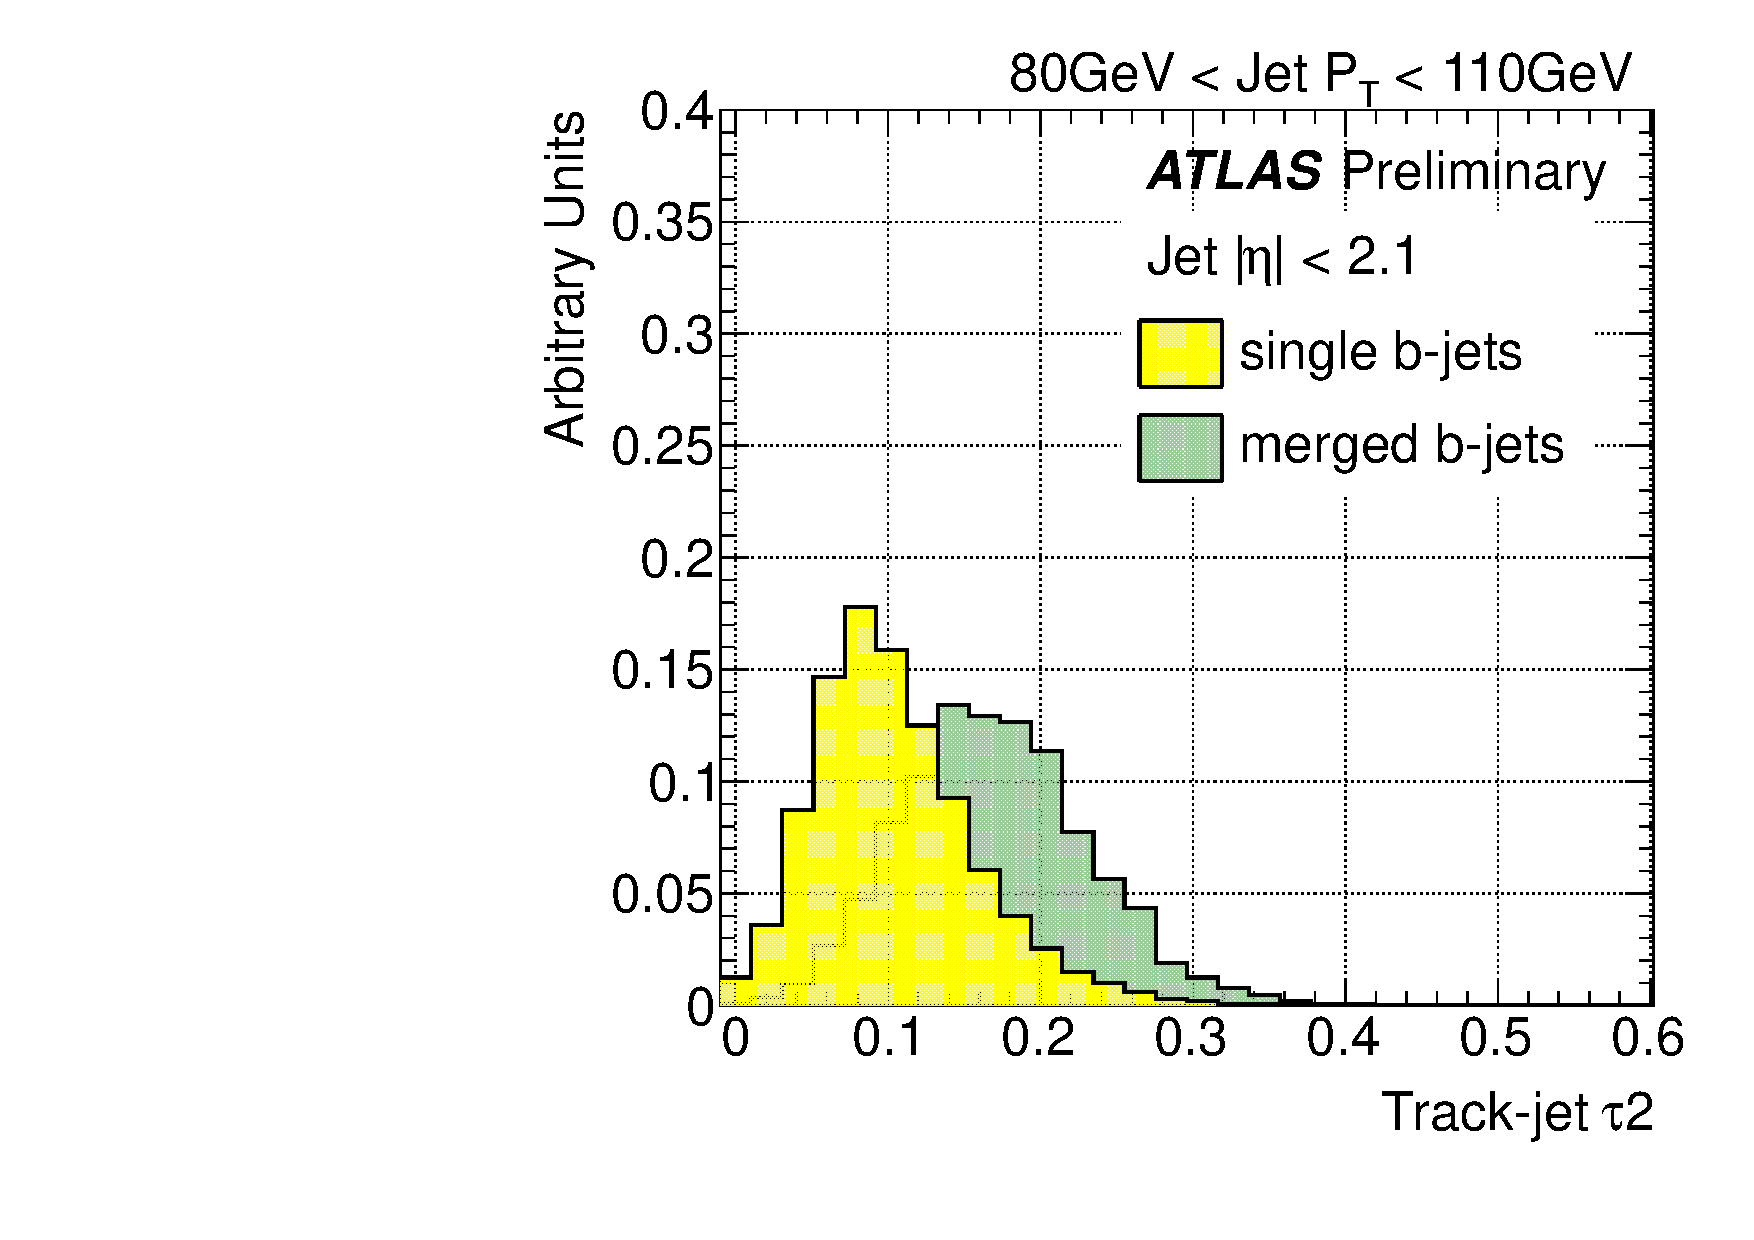
\includegraphics[width=0.49\textwidth]{FIGS/VarsSingleMerged/Tau2080.pdf}
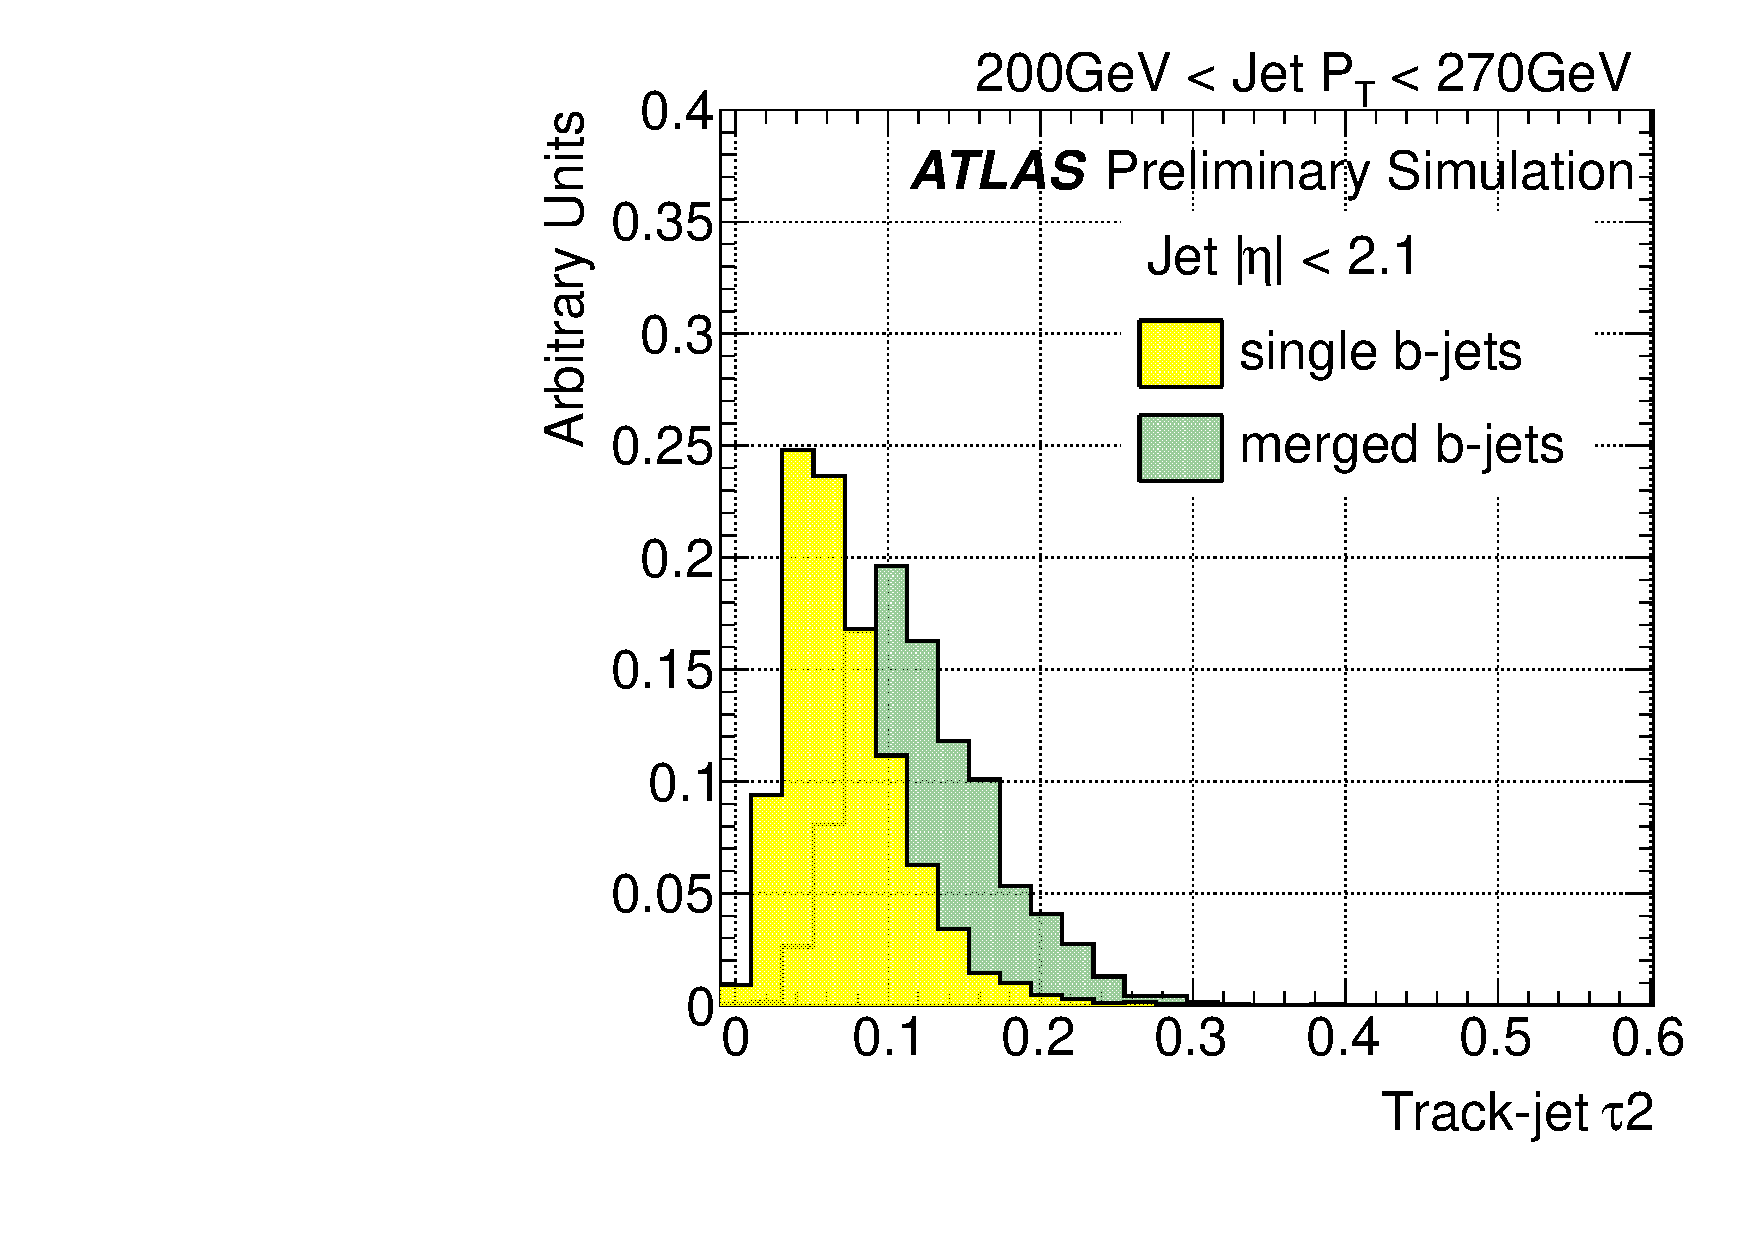
\includegraphics[width=0.49\textwidth]{FIGS/VarsSingleMerged/Tau2200.pdf}
\caption{Distribution of $\tau_2$ in jets for single and merged $b$-jets between 80~GeV to 110~GeV (left) and 200~GeV to 270~GeV (right).}
\label{fig:tau2singlemerged}
\end{figure}

%\begin{figure}[tp]
%\centering
%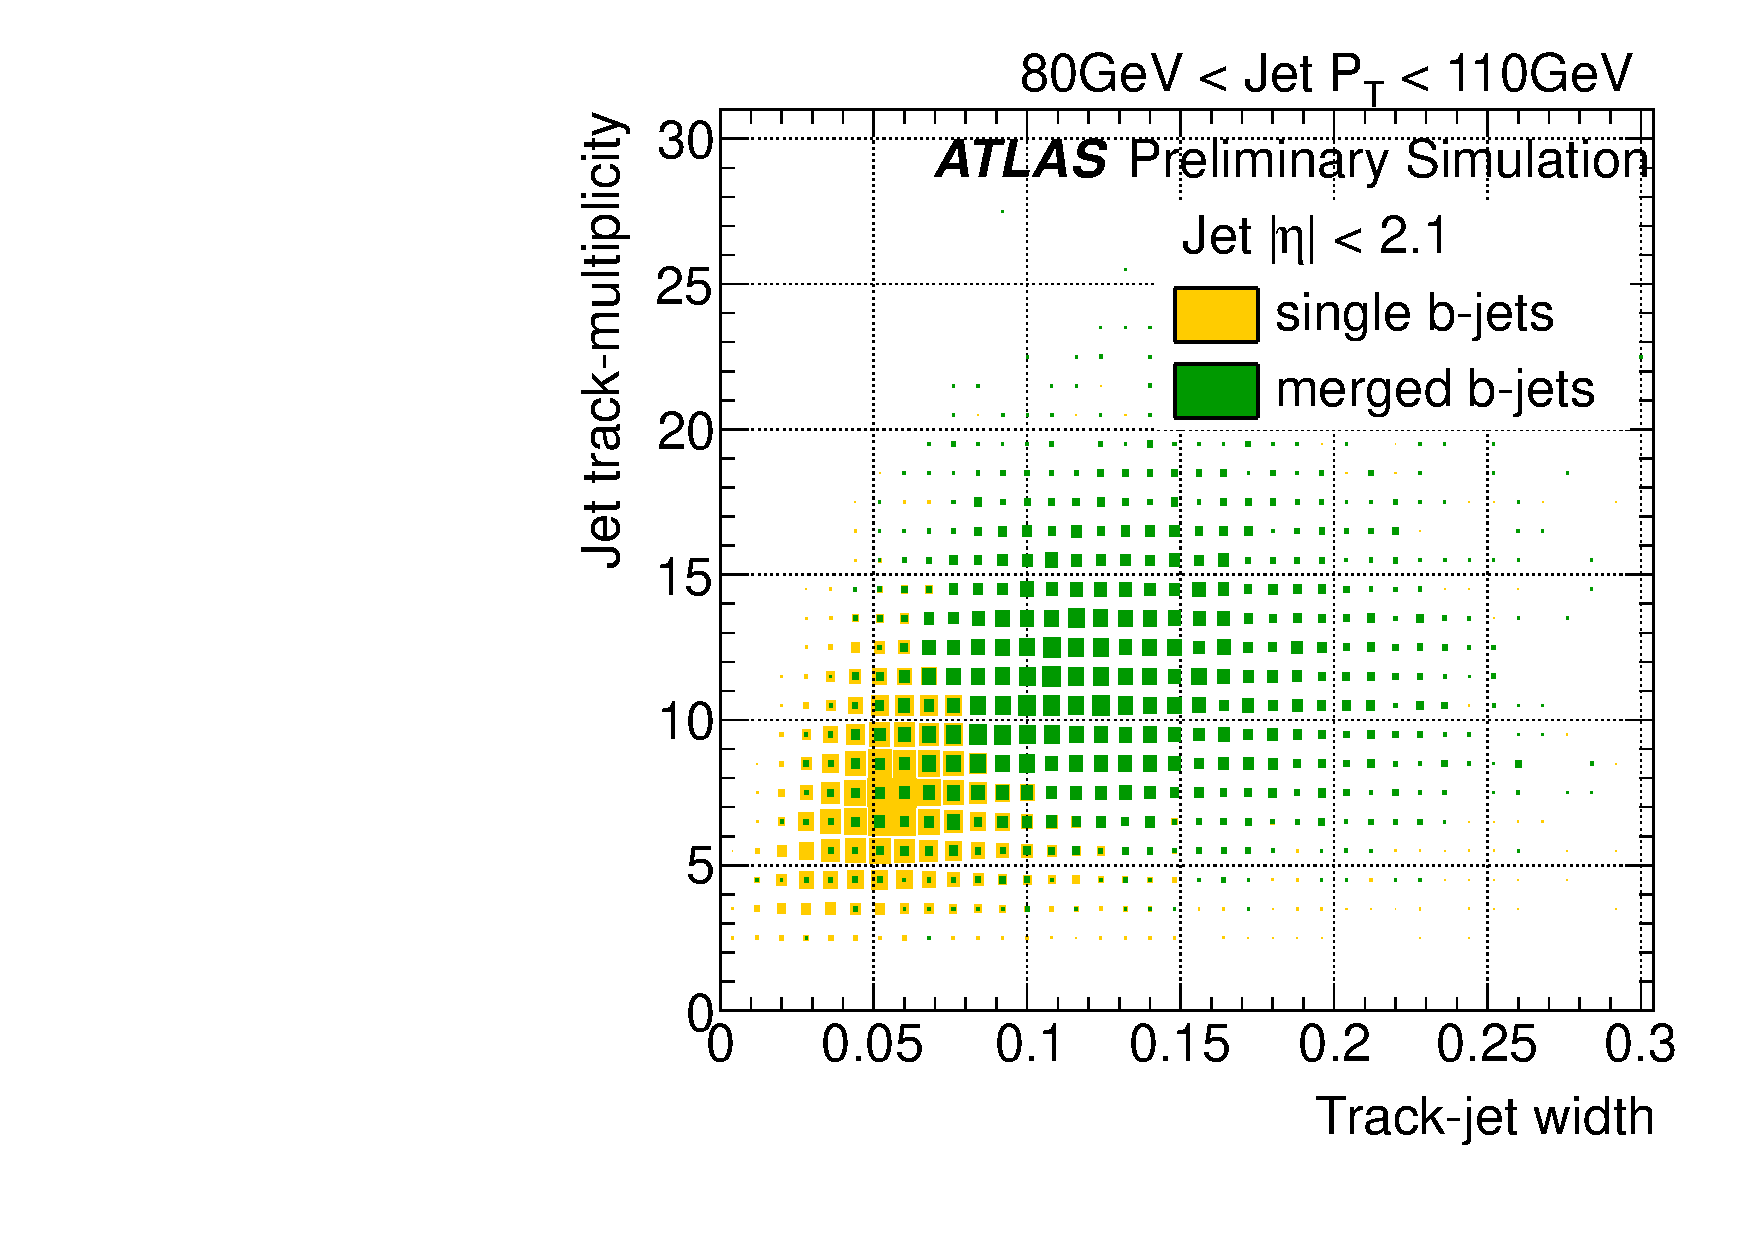
\includegraphics[width=0.49\textwidth]{FIGS/VarsSingleMerged/NtrktrkWidth080.pdf}
%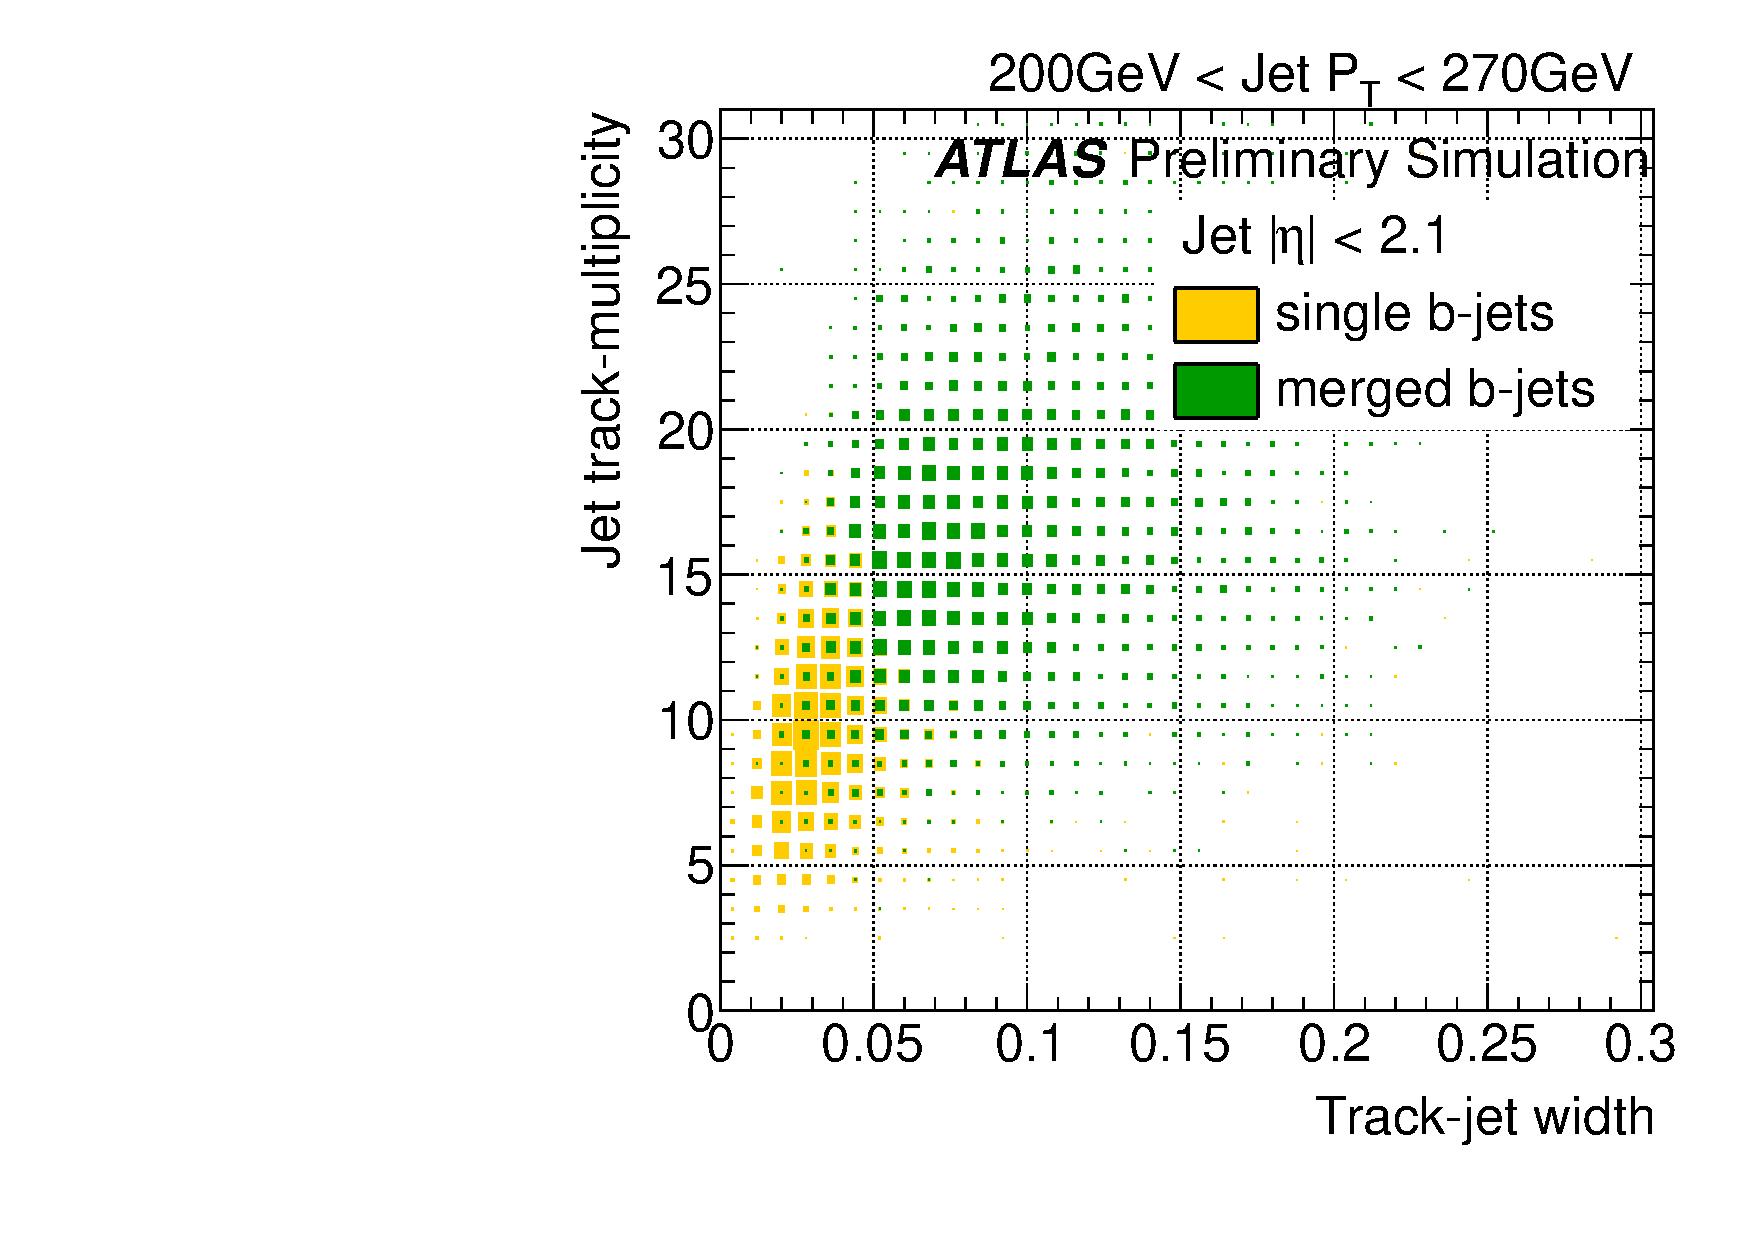
\includegraphics[width=0.49\textwidth]{FIGS/VarsSingleMerged/NtrktrkWidth200.pdf}
%\caption{Correlation between jet track multiplicity and track-jet width for single and merged $b$-jets between 80~GeV to 110~GeV (left) and 200~GeV to 270~GeV (right).}
%\label{fig:ntrktrkwidthsinglemerged}
%\end{figure}

\begin{figure}[tp]
\centering
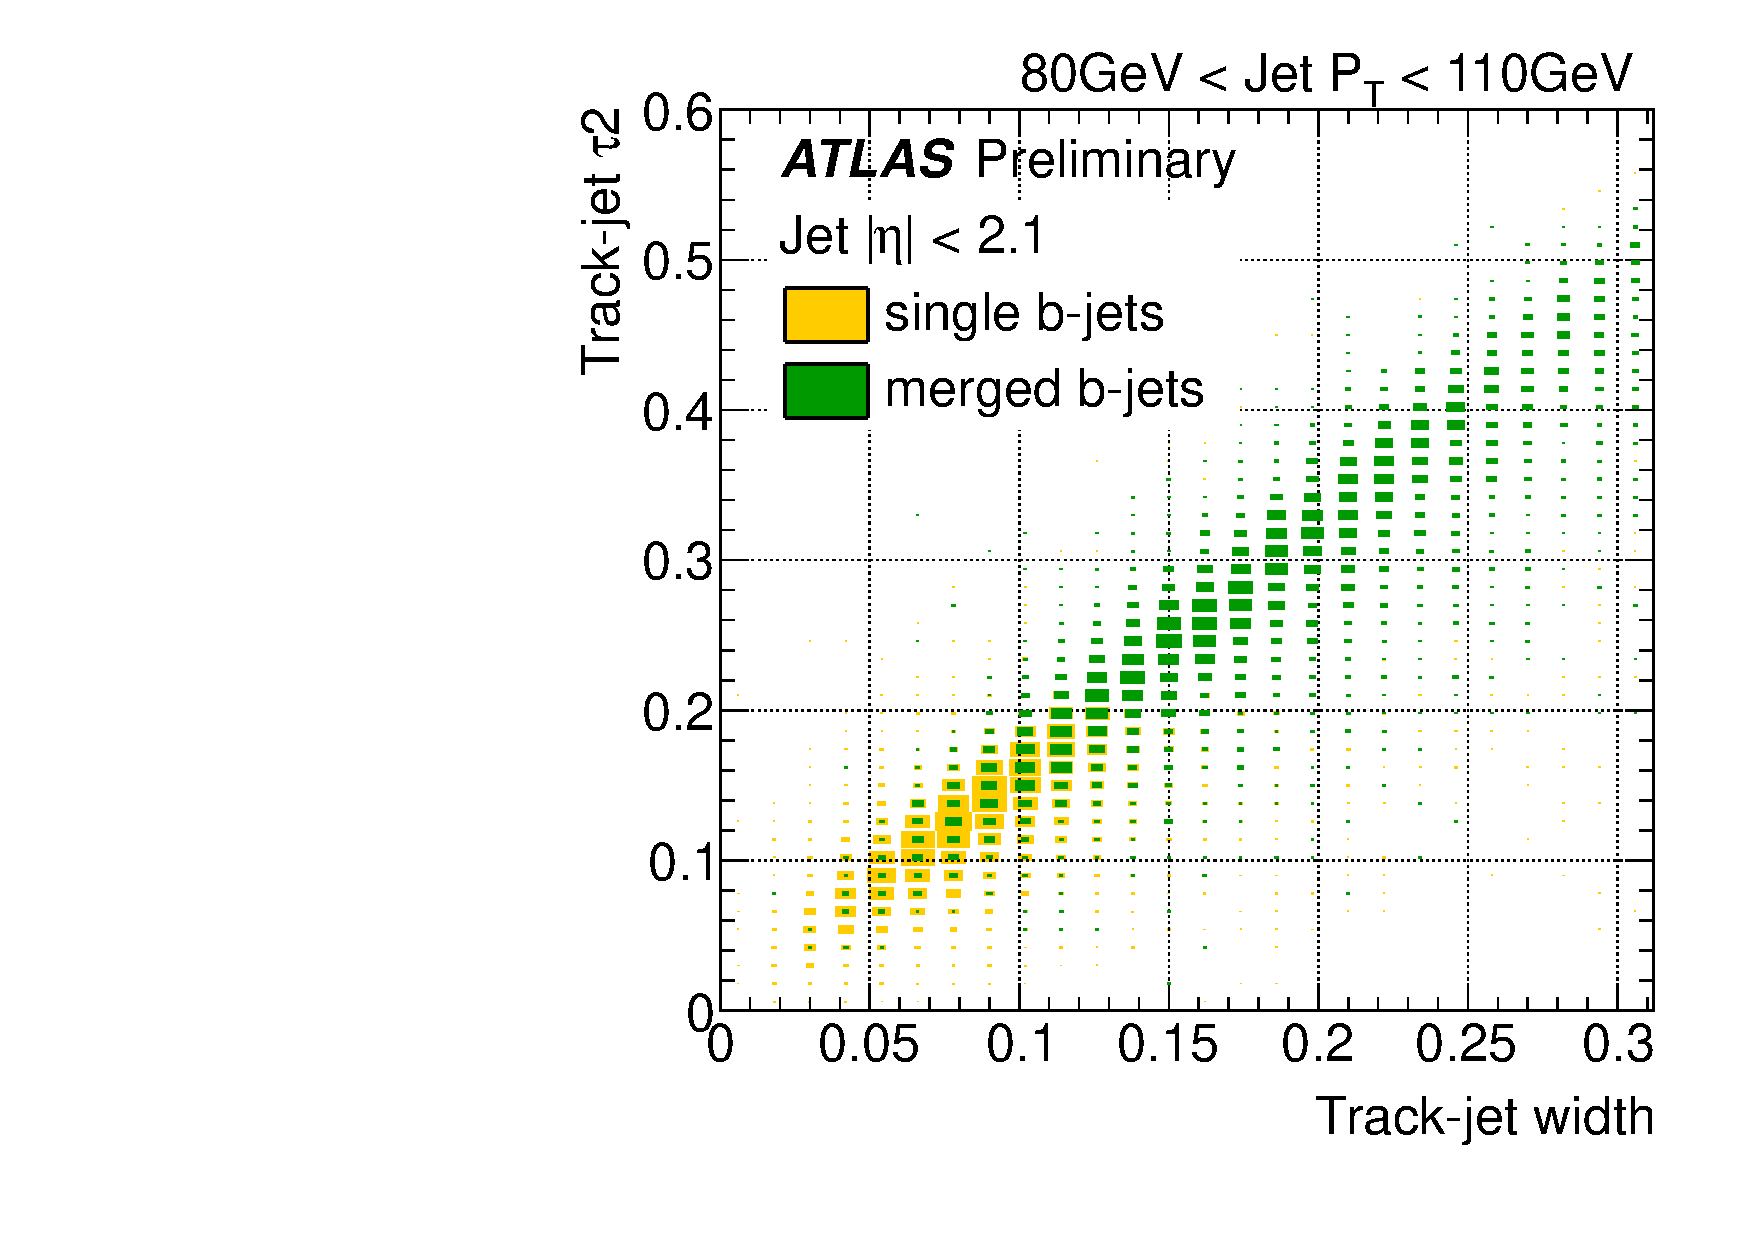
\includegraphics[width=0.49\textwidth]{FIGS/VarsSingleMerged/Tau2trkWidth080.pdf}
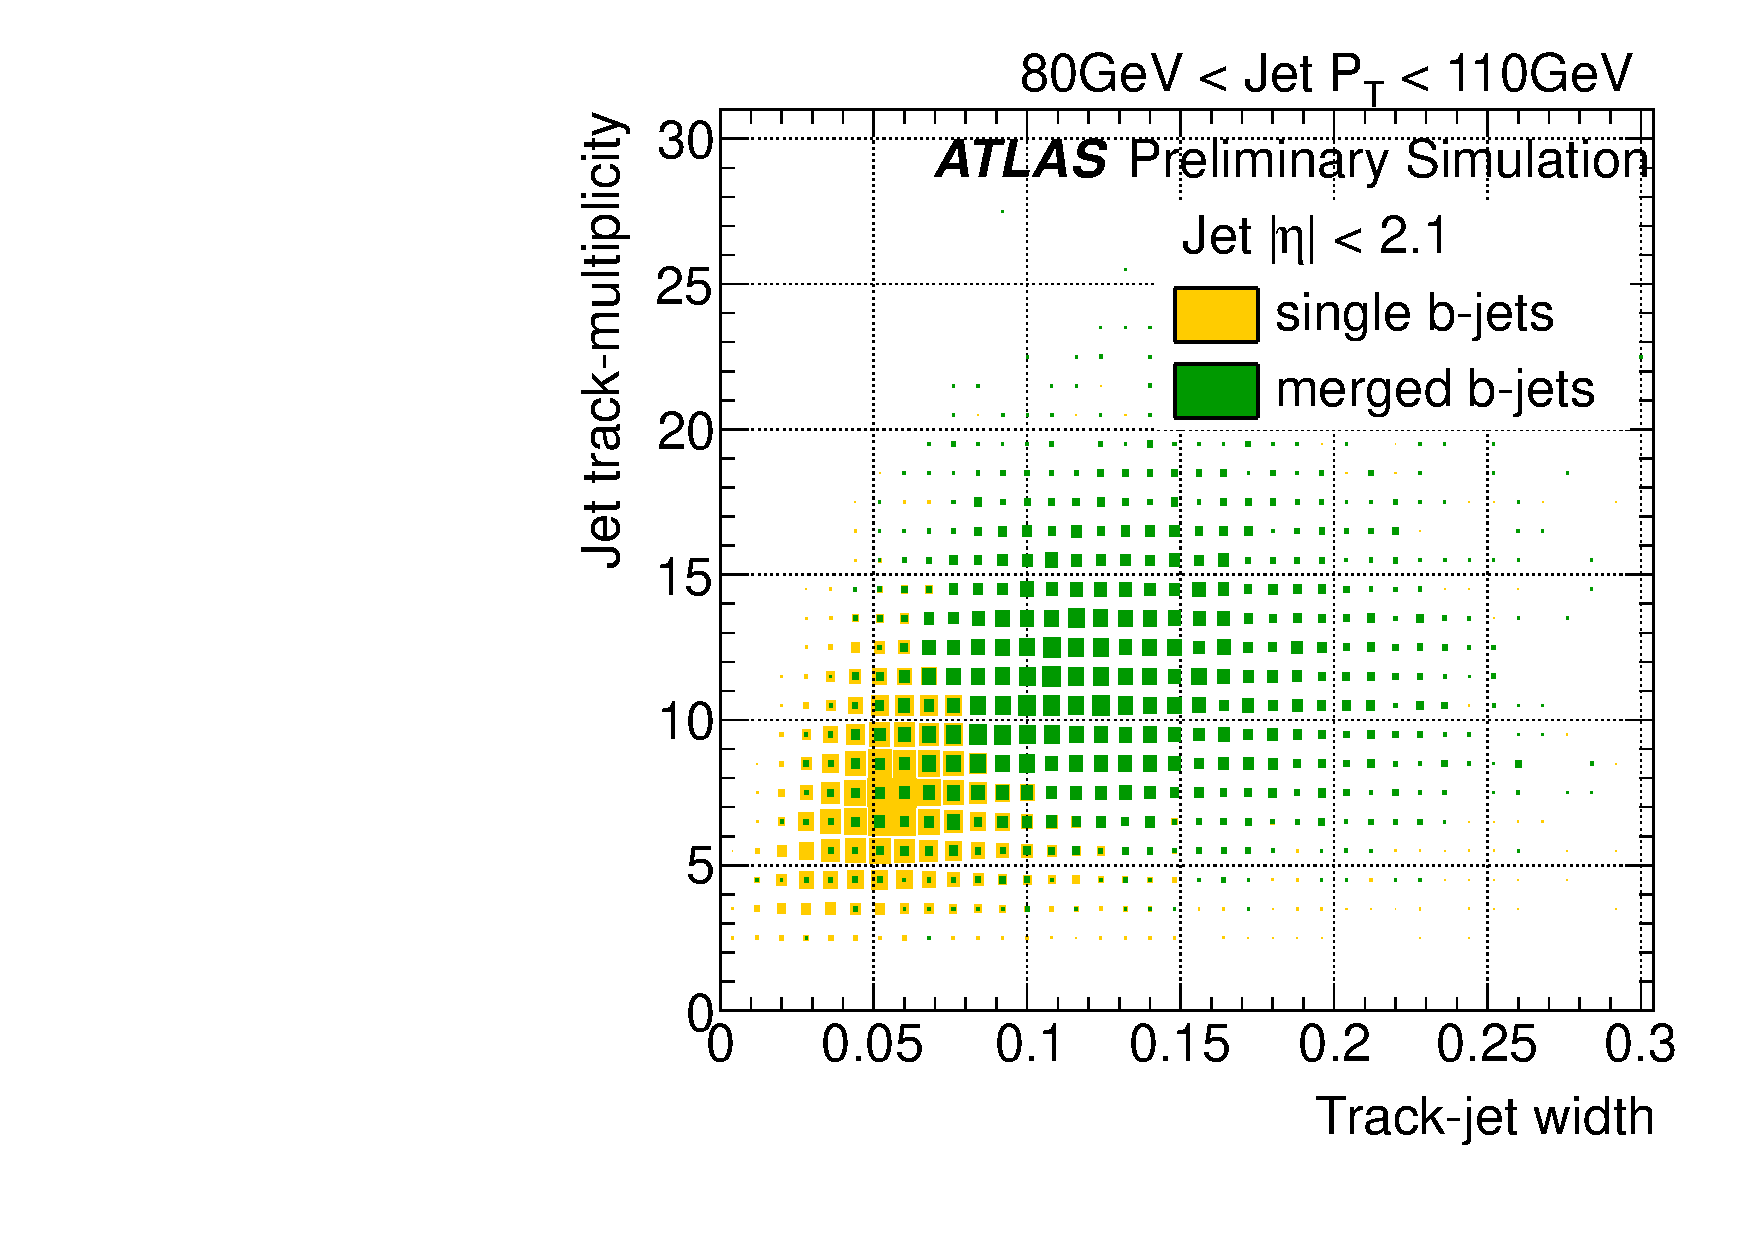
\includegraphics[width=0.49\textwidth]{FIGS/VarsSingleMerged/NtrktrkWidth080.pdf}
\caption{Correlation between $\tau _2$ and track-jet width (left) and jet track multiplicity and track-jet width (right) for single and merged $b$-jets between 80~GeV to 110~GeV. }
\label{fig:tau2trkwidthsinglemerged}
\end{figure}

\begin{figure}[tp]
\centering
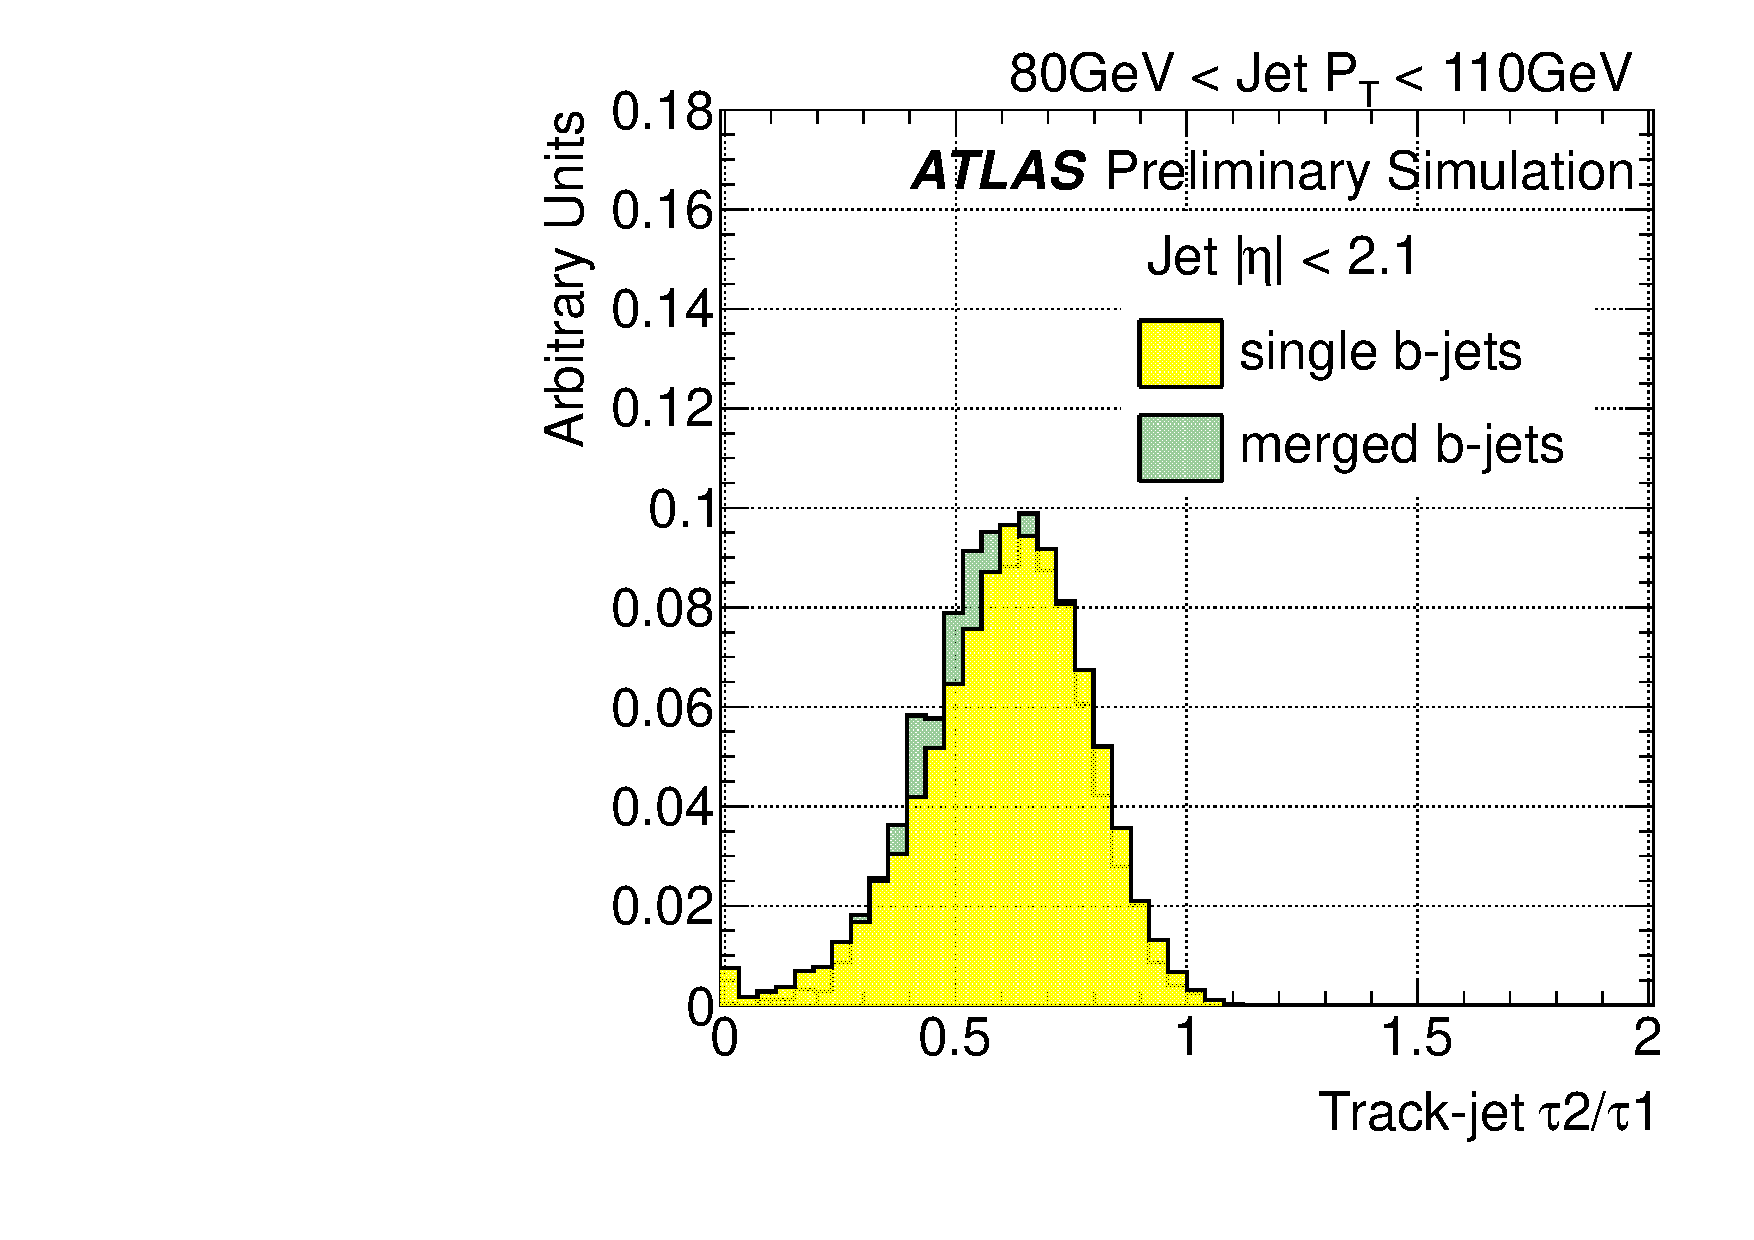
\includegraphics[width=0.49\textwidth]{FIGS/VarsSingleMerged/TauRatio080.pdf}
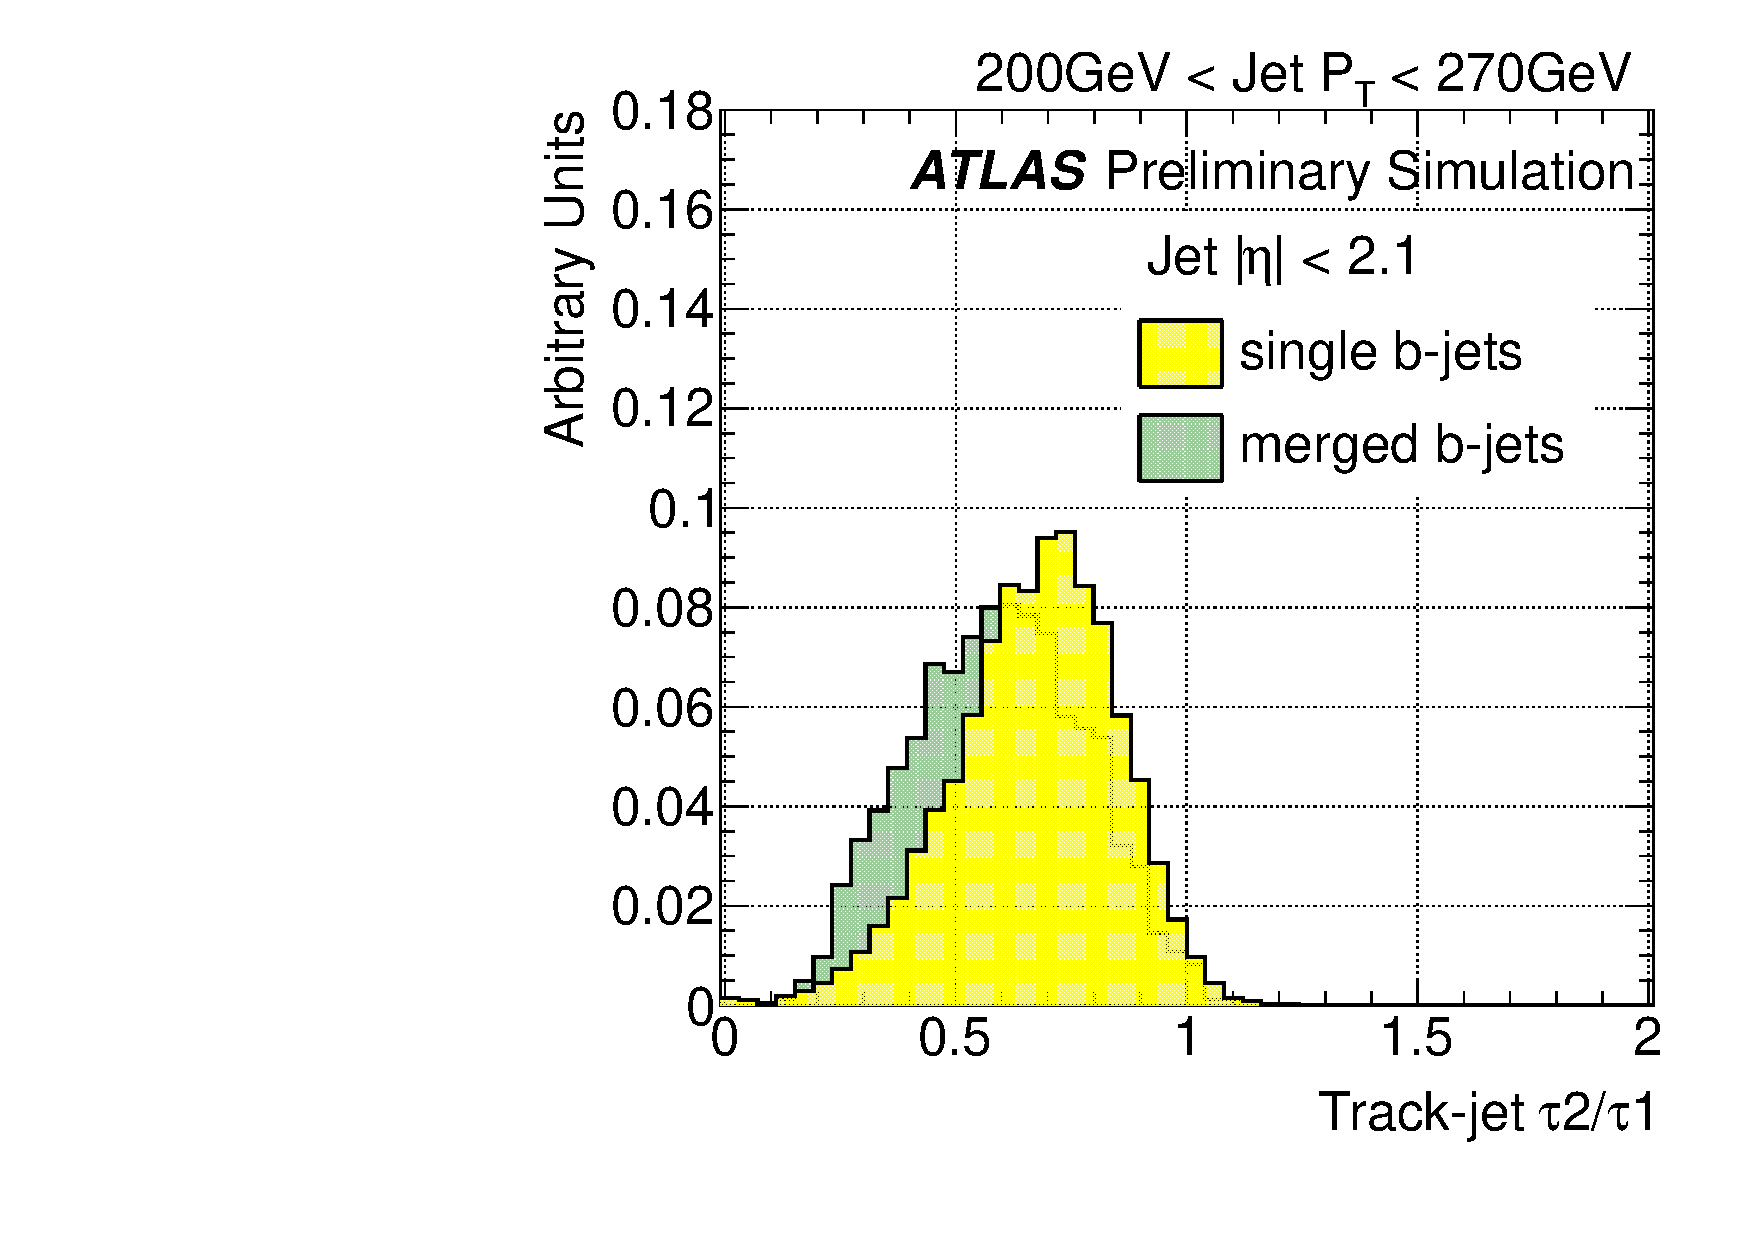
\includegraphics[width=0.49\textwidth]{FIGS/VarsSingleMerged/TauRatio200.pdf}
\caption{Distribution of $\tau_2/\tau_1$ in jets for single and merged $b$-jets between 80~GeV to 110~GeV (left) and 200~GeV to 270~GeV (right).}
\label{fig:tauratiosinglemerged}
\end{figure}



%%%%%%%%%%%%%%%%%%%%%%%%%%%%%%%%%%%%%%%%%%%%%%%%%%%%%%%%%%%%%%%%%%%%%%%%%%%%%%%%%%%%%%%%%%%%%%%%%%
%{ \em IX. Jet eccentricity}
%\vspace{3 mm}
 
{ \em Jet eccentricity} In defining a jet moment there are several ways to weight the momentum and define the center of the jet. We have defined the jet width as the first moment of the transverse energy with respect to the jet axis; another example of useful combination is the jet pull~\cite{PhysRevLett.105.022001}. But it is also natural to look at higher moments, such as those contained in the $2 \times 2$ matrix,
%\[ C = \sum_{i\in jet}\frac{p^i_T|r_i|}{p^{jet}_T} \left( \begin{array}{cc}
% \Delta y^2_i & \Delta y_i \Delta\phi_i \\ 
% \Delta\phi_i \Deltay_i & \Delta \phi^2_i \end{array} \right). \]
%
\begin{equation}
 \begin{bmatrix}
 \sum E_i \eta^2_i       &  -\sum E_i \eta_i \phi_i \\ 
-\sum E_i \eta_i \phi_i &  \sum E_i \phi^2_i \right
 \end{bmatrix}
\end{equation}
%
Here, $(E_i,\eta_i,\phi_i)$ are the jet constituent energy, pseudorapidity and azimuthal angle, respectively. The eigenvalues $\lambda_m \geq \lambda_p $ of this tensor are associated to the semiminor and semimajor axes of an elliptical jet, in the $\eta - \phi$ plane. The jet eccentricity, defined below, is a combination of these eigenvalues, and it is a measure of how elongated is the area of a jet,
%
\begin{equation} 
e = \sqrt{1-r^2}
\label{ecc}
\end{equation}
%
where the parameter $r$ is defined as the ratio of the eigenvalues,
%
\begin{equation} 
r = \frac{\lambda_m}{\lambda_p} = \frac{\sum E_i \eta^2_i+\sum E_i \phi^2_i - \sqrt{(\sum E_i \eta^2-\sum E_i \phi^2_i)^2+4(\sum E_i \eta_i \phi_i)^2}}{\sum E_i \eta^2_i+\sum E_i \phi^2_i + \sqrt{(\sum E_i \eta^2-\sum E_i \phi^2_i)^2+4(\sum E_i \eta_i \phi_i)^2}}.
\label{ecc2}
\end{equation}
%
%For circular jets, $e = 0$. 
%No significan difference in eccentricity was found between quark and gluon jets.
Figure~\ref{fig:jeteccsinglemerged} shows the distribution of the jet eccentricity, built using track constituents. No significant difference in eccentricity was found between single and merged $b$-jets. 
%\vspace{3 mm}

\begin{figure}[tp]
\centering
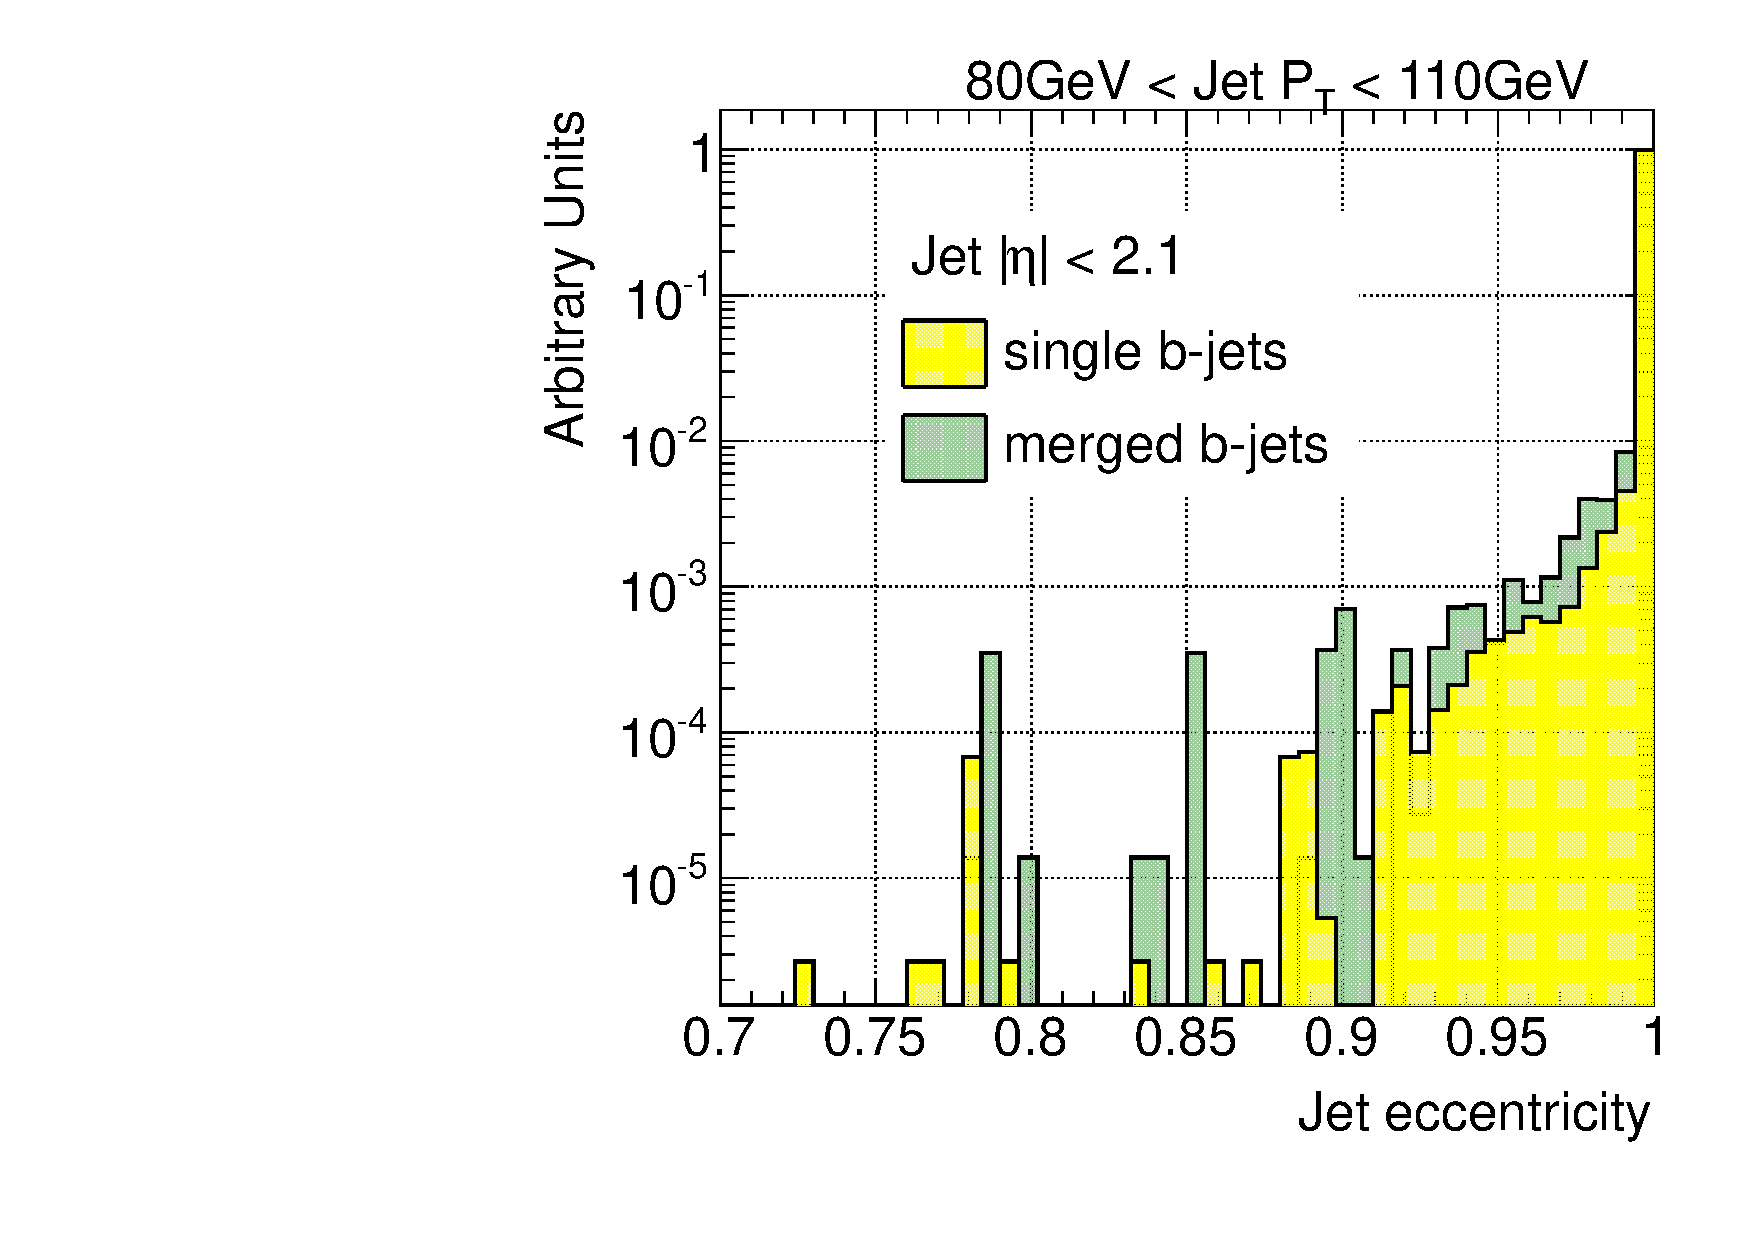
\includegraphics[width=0.49\textwidth]{FIGS/VarsSingleMerged/JetEcc080.pdf}
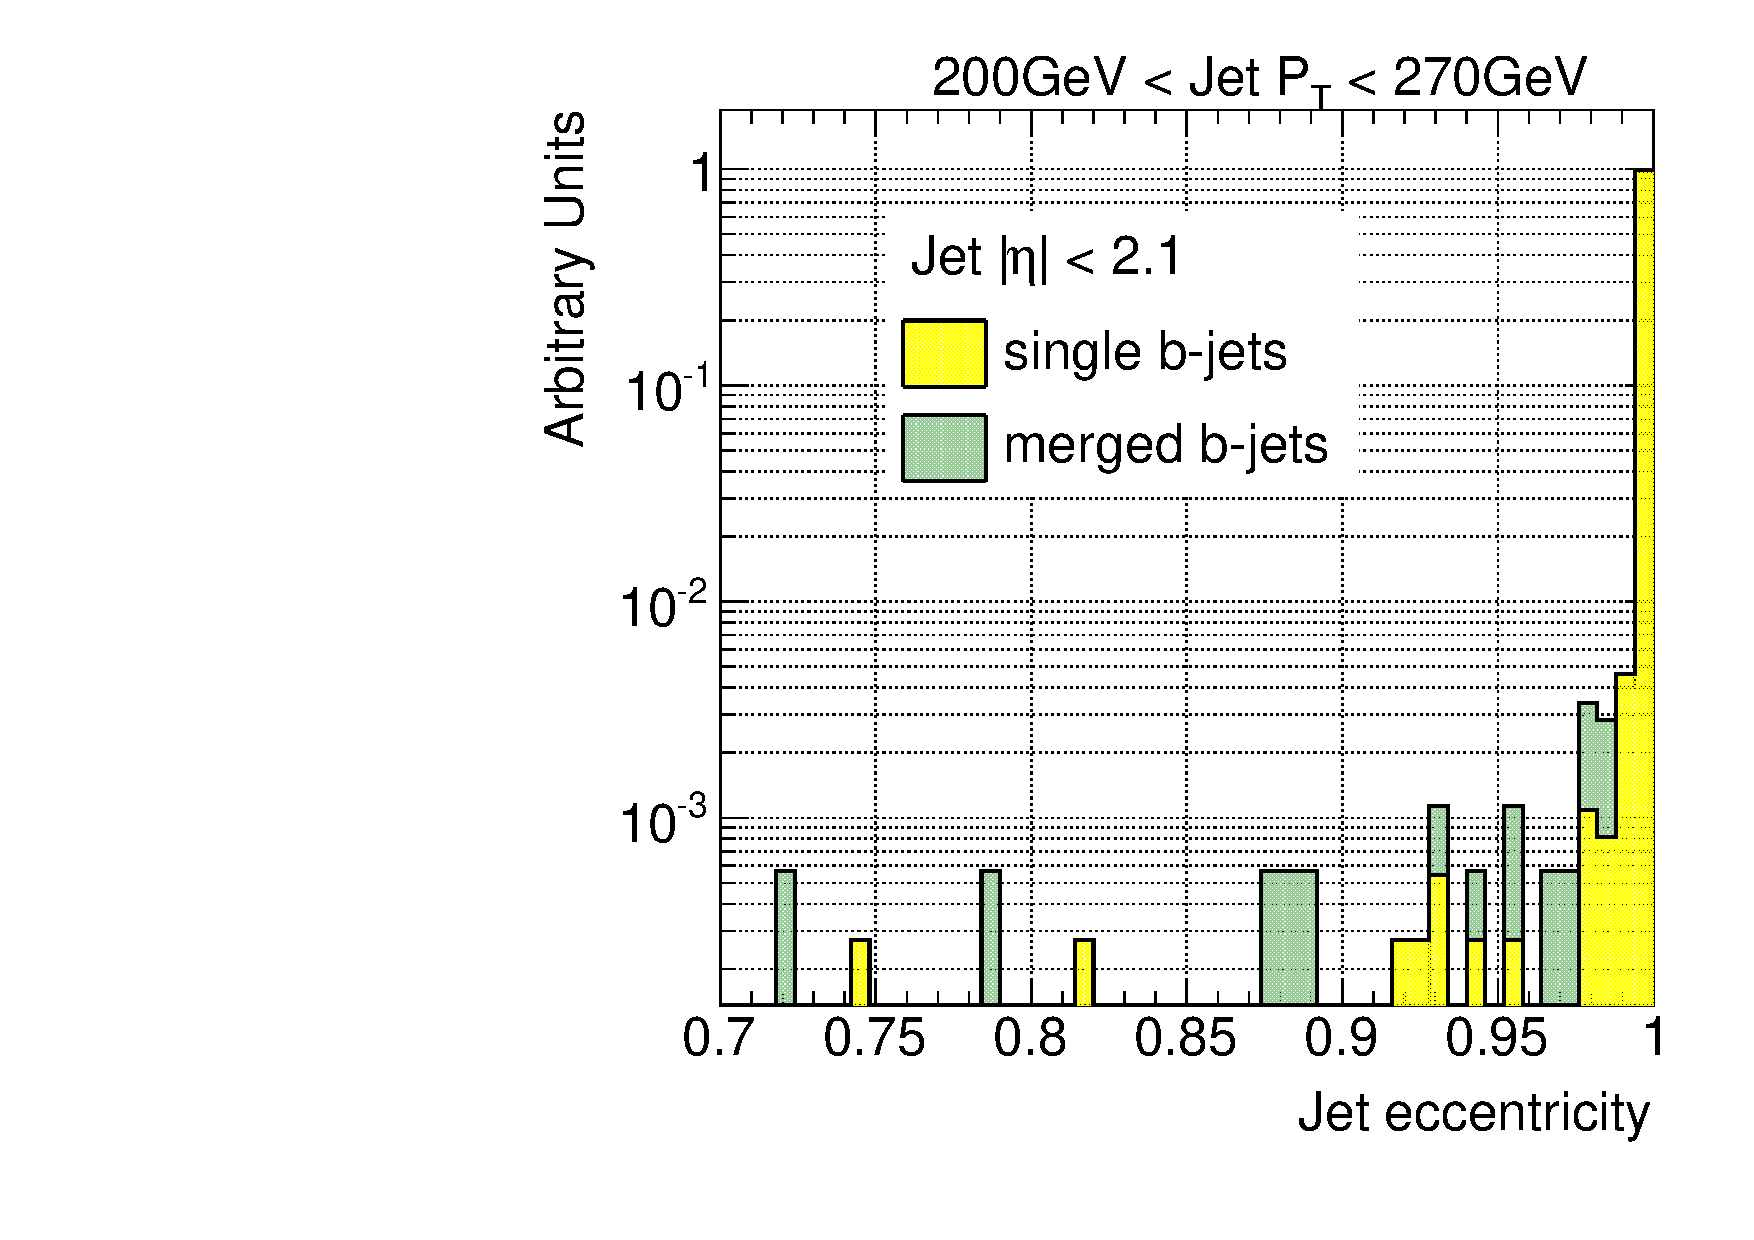
\includegraphics[width=0.49\textwidth]{FIGS/VarsSingleMerged/JetEcc200.pdf}
\caption{Distribution of the jet eccentricity for single and merged $b$-jets between 80~GeV to 110~GeV (left) and 200~GeV to 270~GeV (right).}
\label{fig:jeteccsinglemerged}
\end{figure}







\subsubsection{Further studies}%``ghost-association'' and bigger cone jets}

In order to better understand the behavior observed for $\tau_2$, $\tau_2/tau_1$ and jet eccentricity in anti-$k_T$ 0.4 jets, these variables were studied for other two different scenarios,

\begin{itemize}\addtolength{\itemsep}{-0.4\baselineskip}
\item 
using the active area of jets (with clusters used as input to jet reconstruction).
\item
using bigger 0.6 anti-$k_T$ jets
\end{itemize}
%
in order to enhance the efficiency to capture the decay products in gluon to $b \bar{b}$-jets.

Figures~\ref{fig:tau2GhostAndAntikt6} to~\ref{fig:jeteccGhostAndAntikt6} show distributions of variables mentioned above for single and merged $b$-jets  between 80~GeV to 110~GeV.

\begin{figure}[tp]
\centering
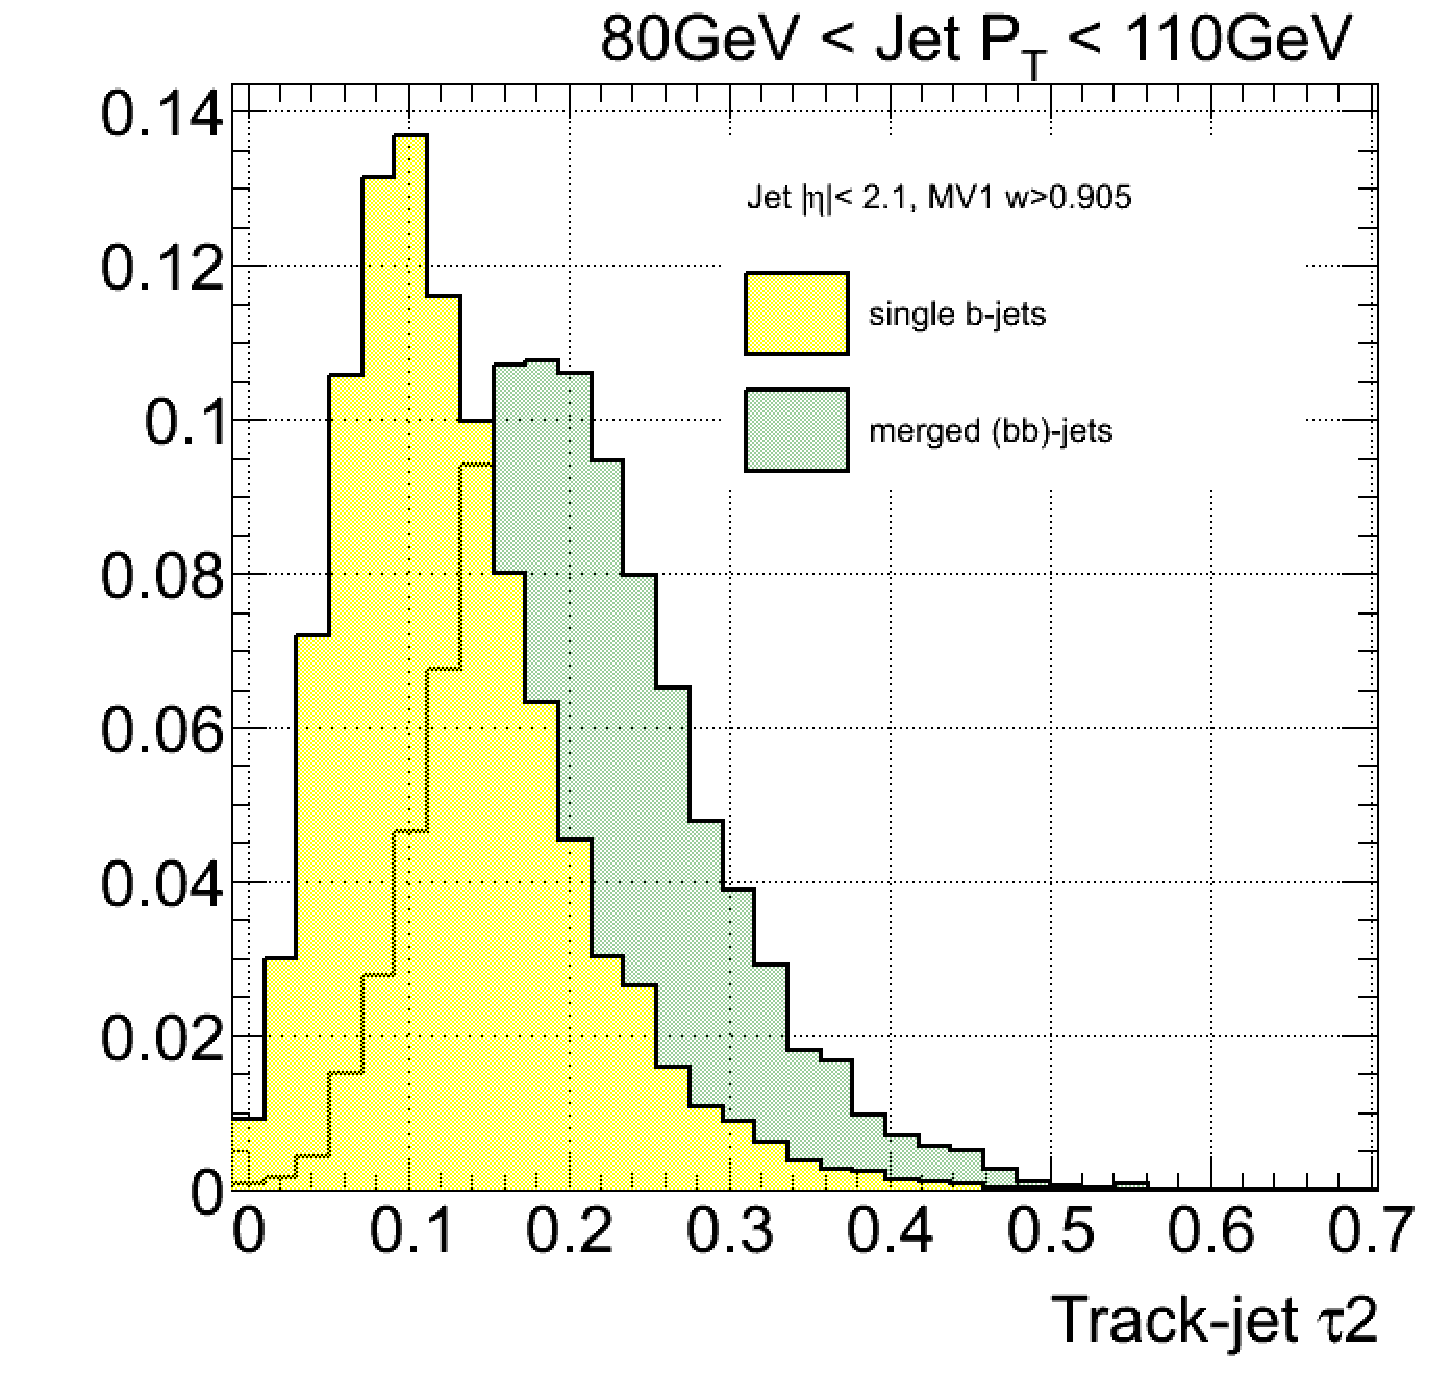
\includegraphics[width=0.49\textwidth]{FIGS/TEMPFigs/Antikt6VarsSingleMerged/Tau2080.pdf}
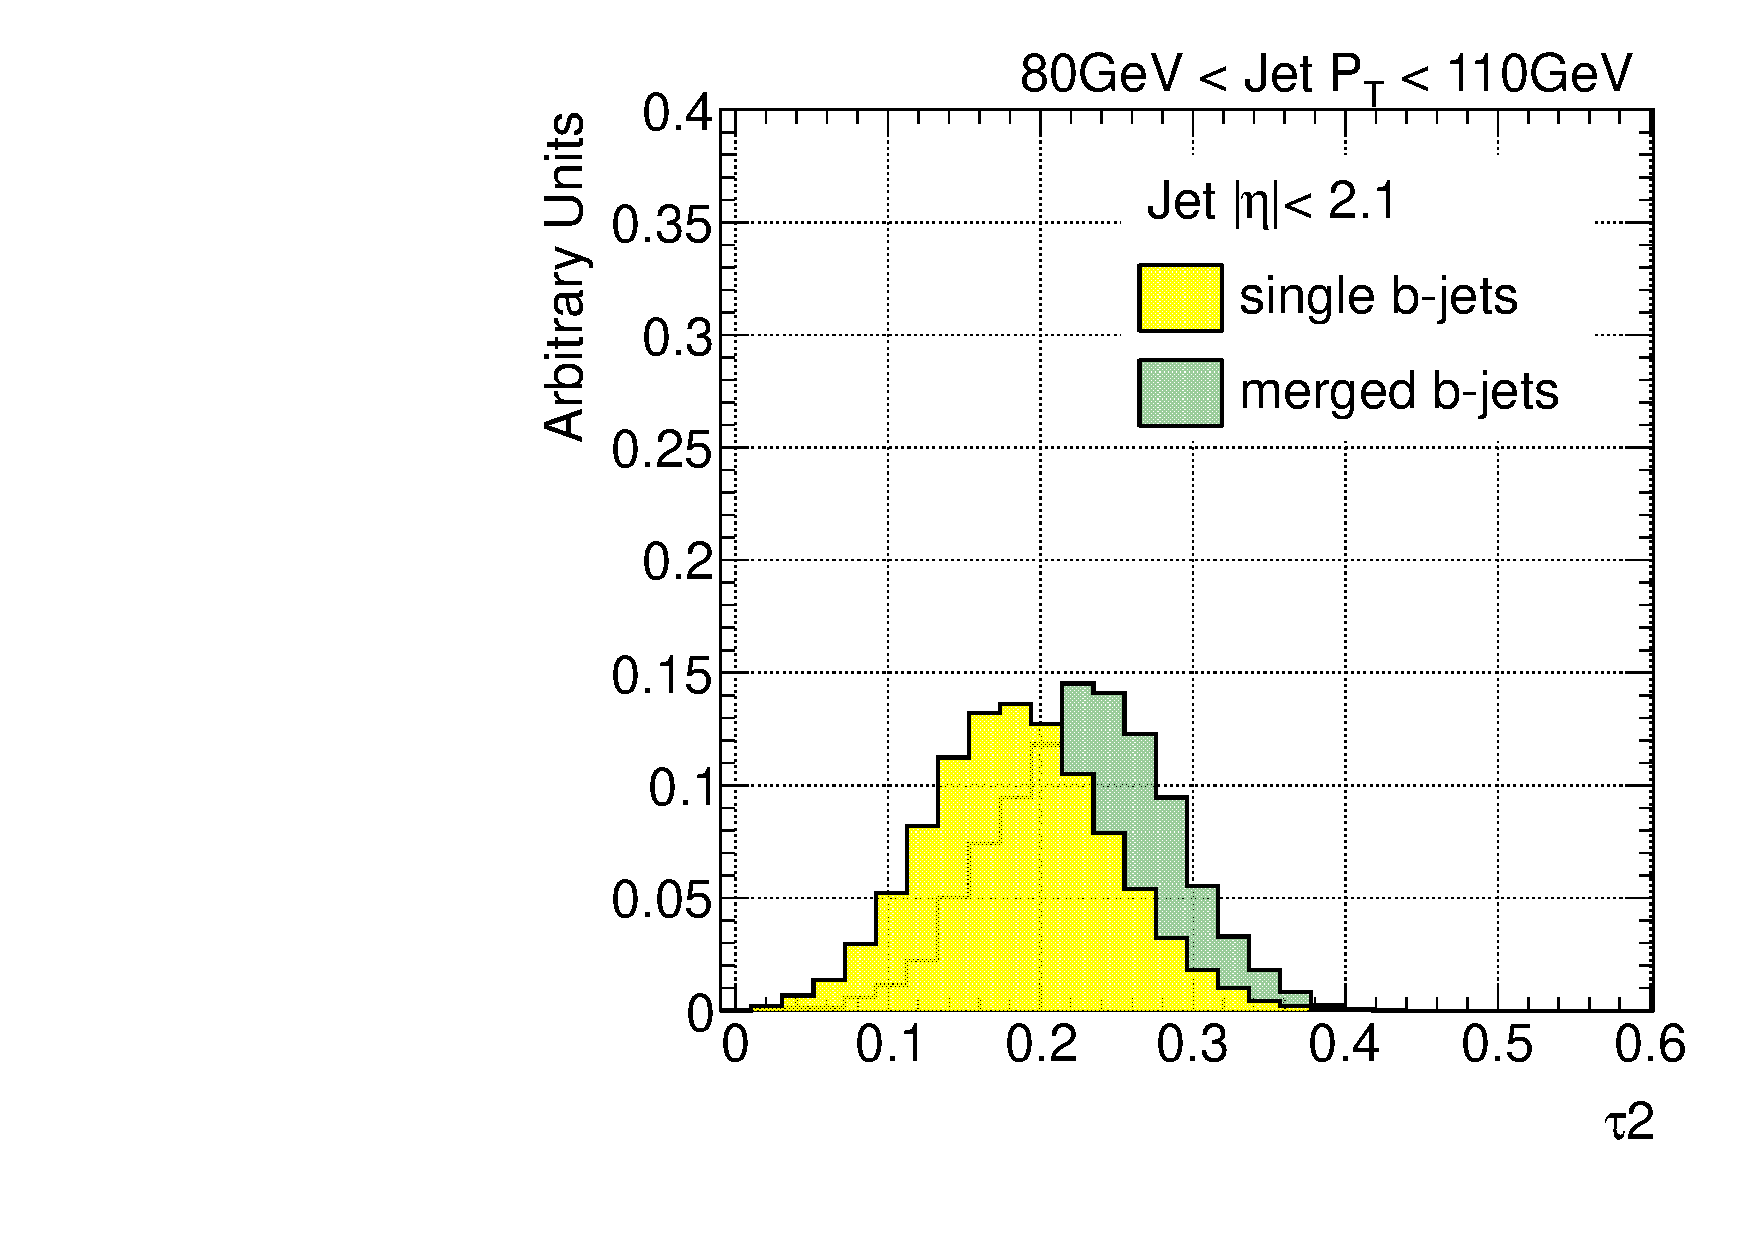
\includegraphics[width=0.49\textwidth]{FIGS/TEMPFigs/GhostMatchingVarsClus/Tau2080.pdf}
\caption{Distribution of $\tau_2$ for single and merged $b$-jets between 80~GeV to 110~GeV in anti-$k_T$ 0.6 jets using track constituents (left) and anti-$k_T$ 0.4 jets using the active area of the jet, with calorimeter topoclusters as input.}
\label{fig:tau2GhostAndAntikt6}
\end{figure}

\begin{figure}[tp]
\centering
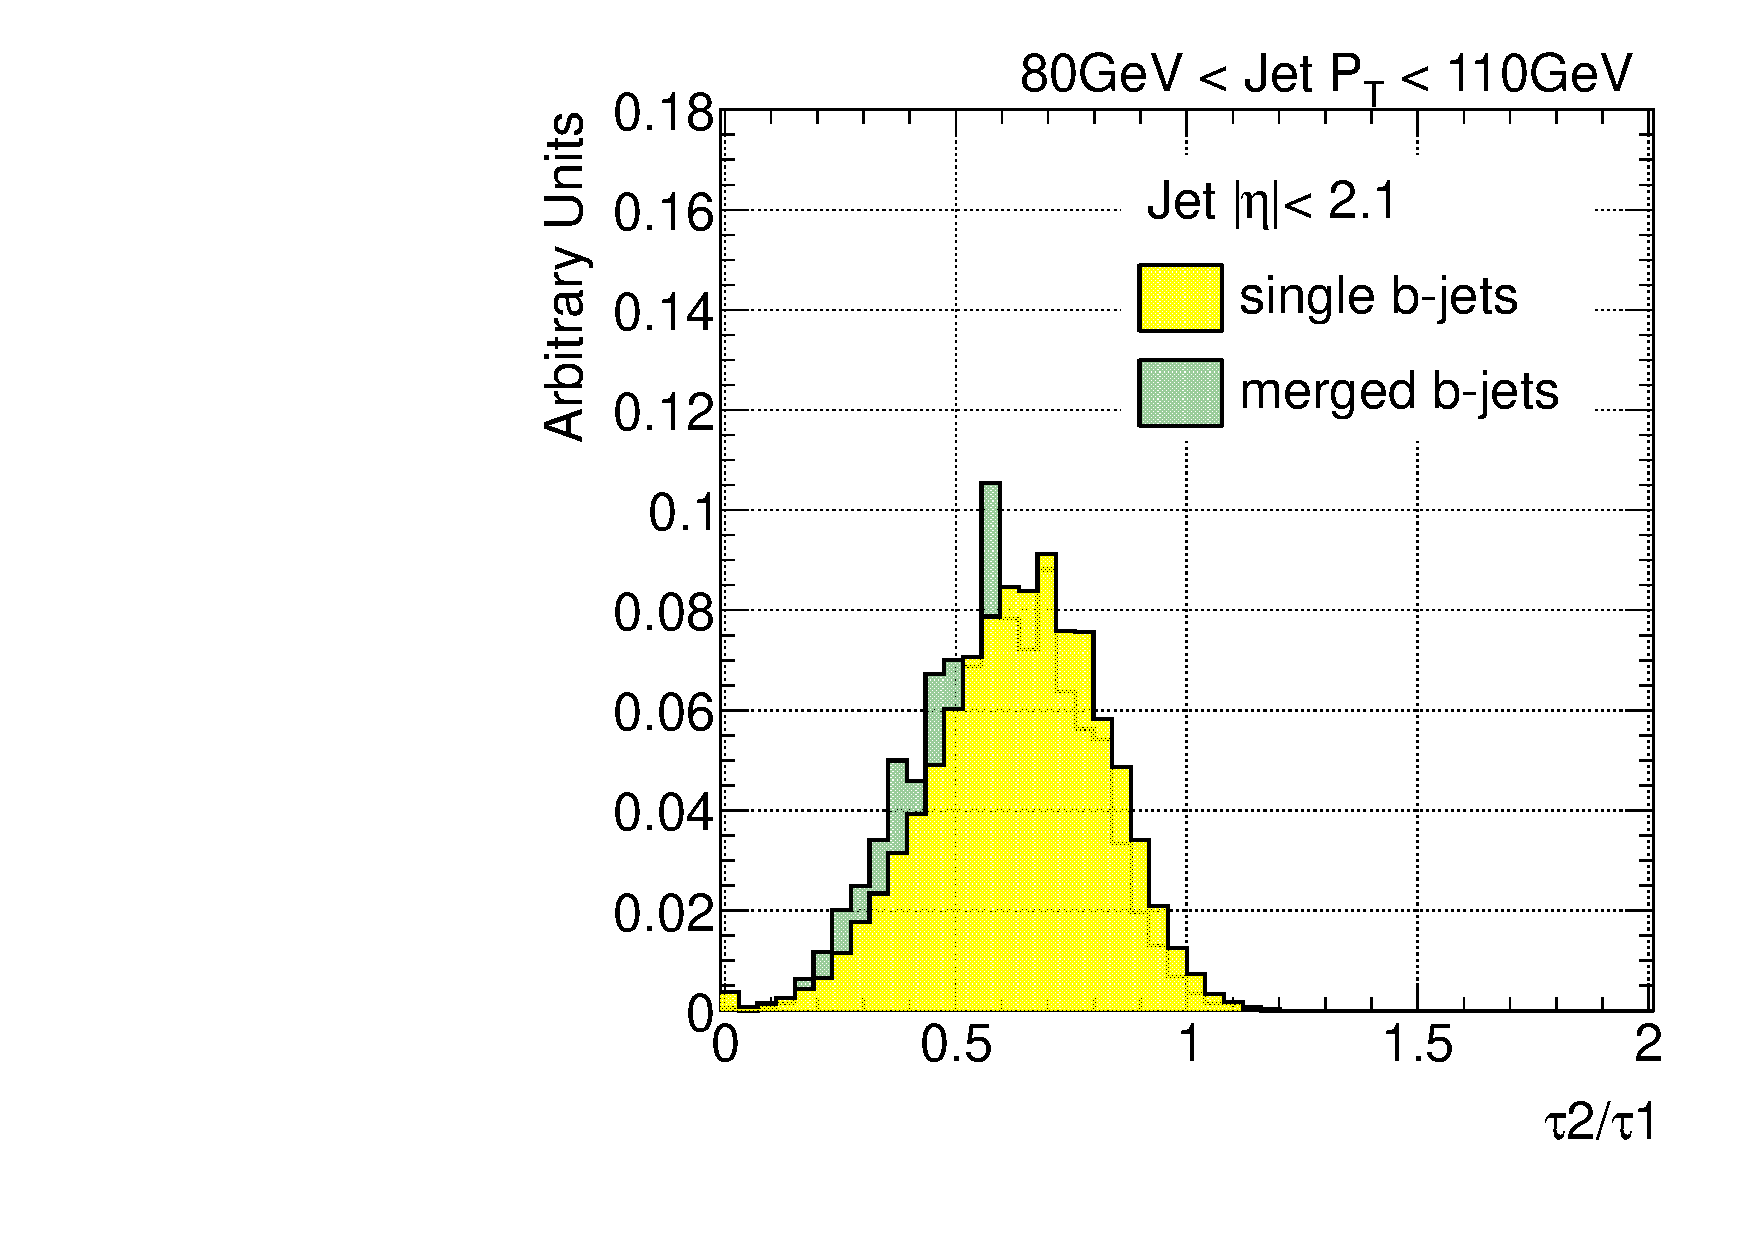
\includegraphics[width=0.49\textwidth]{FIGS/TEMPFigs/Antikt6VarsSingleMerged/Tauratio080.pdf}
\includegraphics[width=0.49\textwidth]{FIGS/TEMPFigs/GhostMatchingVarsClus/Tauratio2080.pdf}
\caption{Distribution of $\tau_2/\tau_1$ for single and merged $b$-jets between 80~GeV to 110~GeV in anti-$k_T$ 0.6 jets using track constituents (left) and anti-$k_T$ 0.4 jets using the active area of the jet, with calorimeter topoclusters as input.}
\label{fig:tau2GhostAndAntikt6}
\end{figure}

%\begin{figure}[tp]
%\centering
%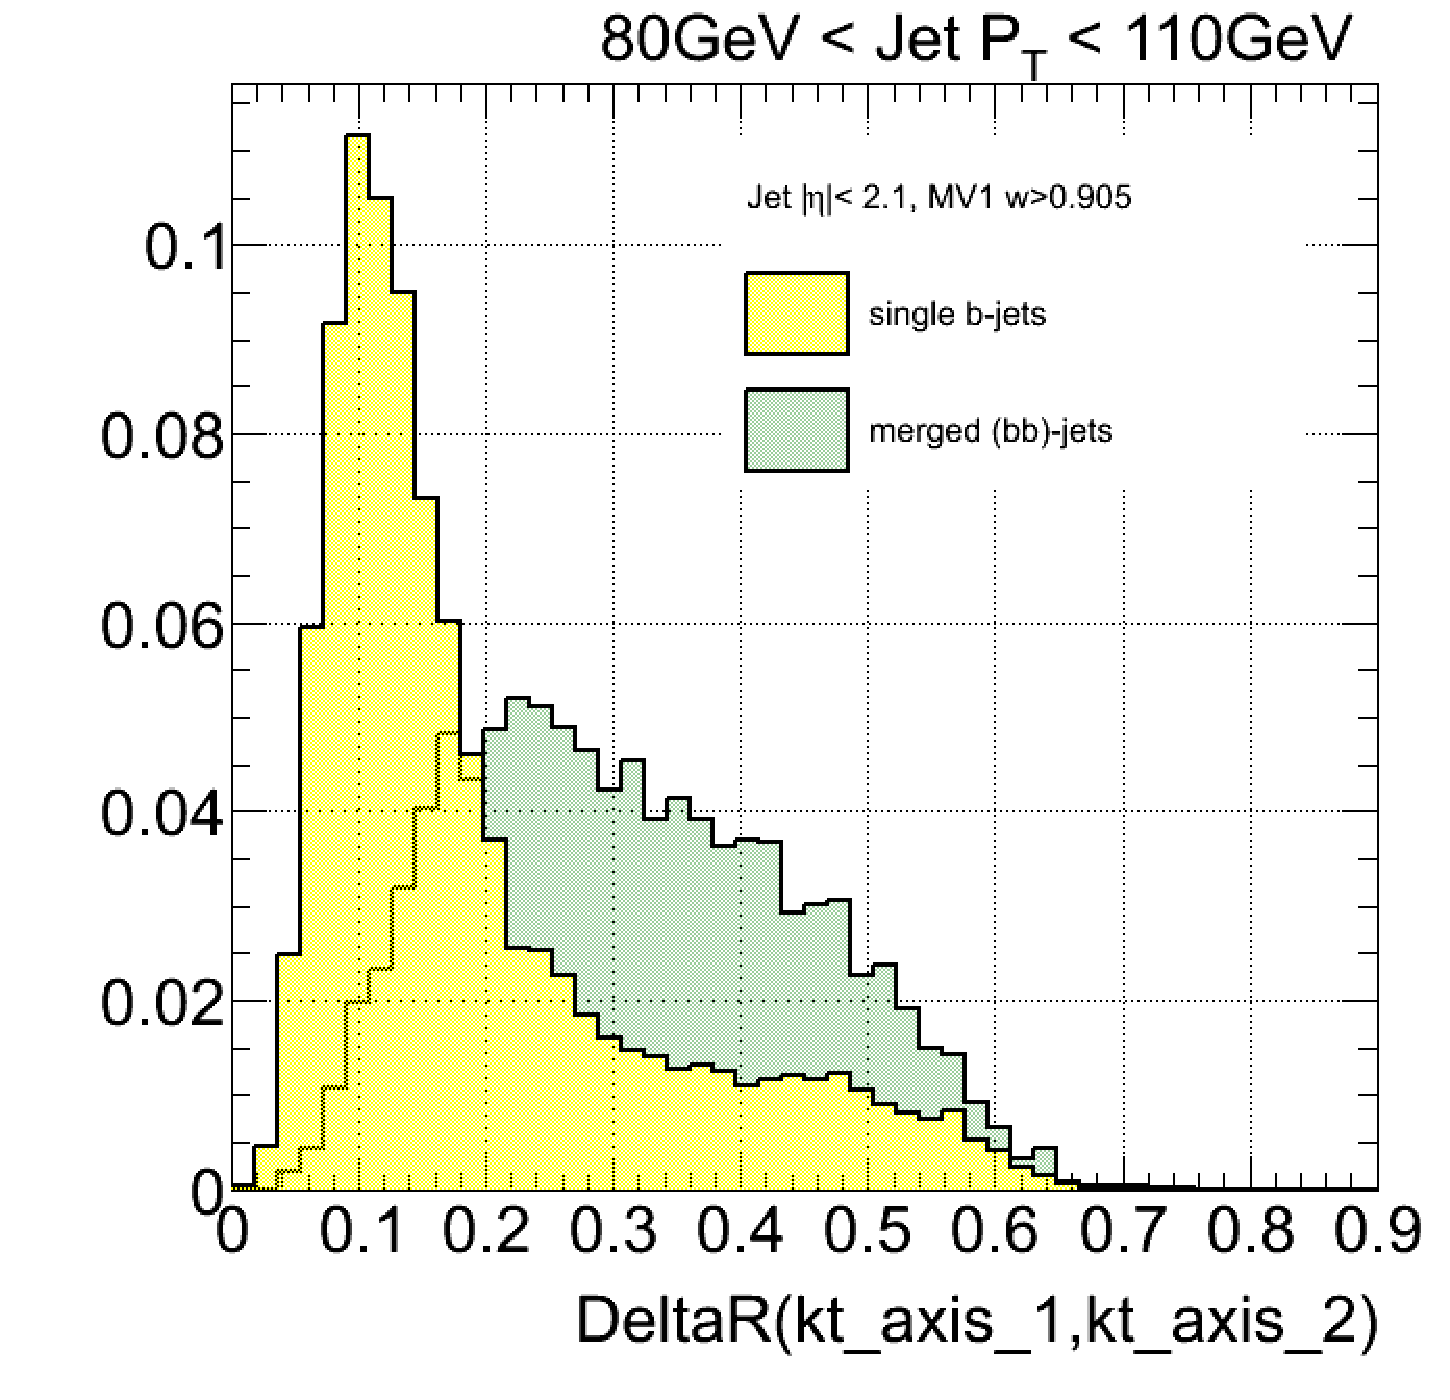
\includegraphics[width=0.49\textwidth]{FIGS/TEMPFigs/Antikt6VarsSingleMerged/DRkt2axes080.pdf}
%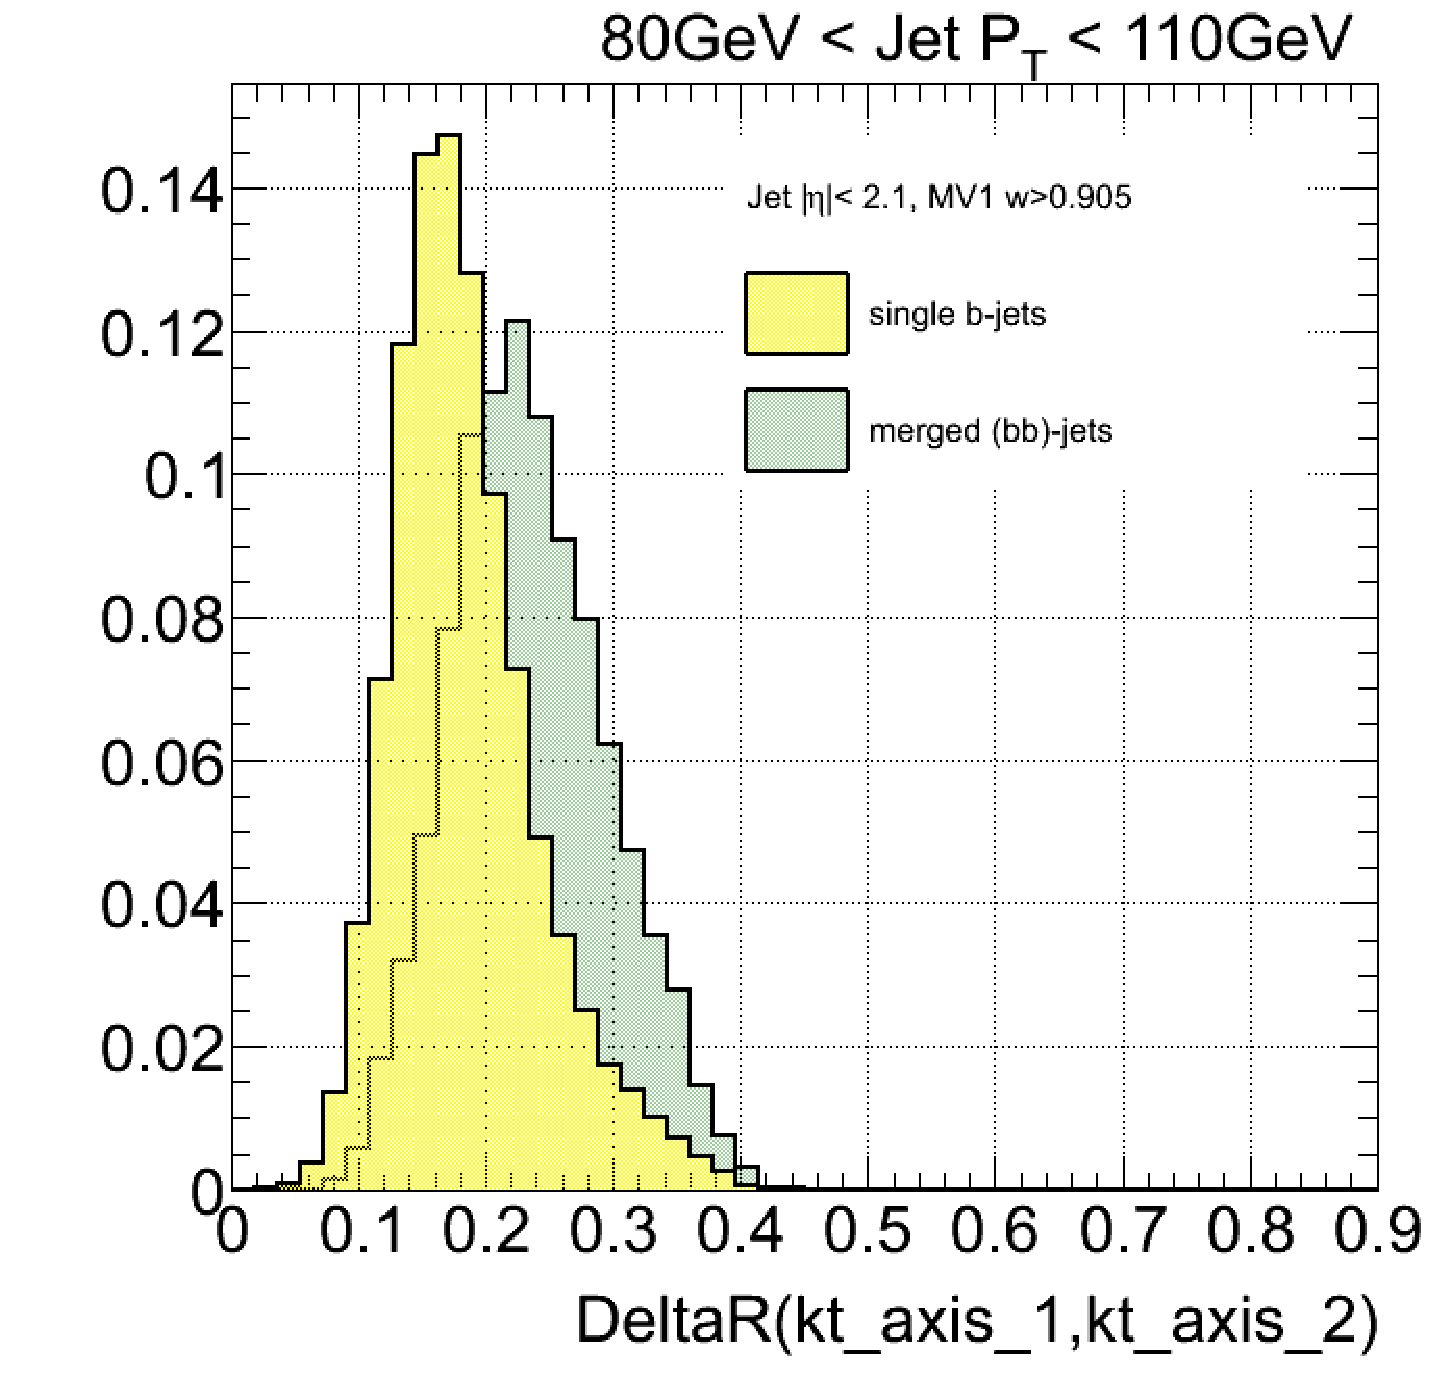
\includegraphics[width=0.49\textwidth]{FIGS/TEMPFigs/GhostMatchingVarsClus/DRkt2axes080.pdf}
%\caption{Distribution of $\Delta R$ between $k_T$ subjets for single and merged $b$-jets between 80~GeV to 110~GeV in anti-$k_T$ 0.6 jets using track constituents (left) and anti-$k_T$ 0.4 jets using the active area of the jet, with calorimeter topoclusters as input.}
%\label{fig:drktaxisGhostAndAntikt6}
%\end{figure}

\begin{figure}[tp]
\centering
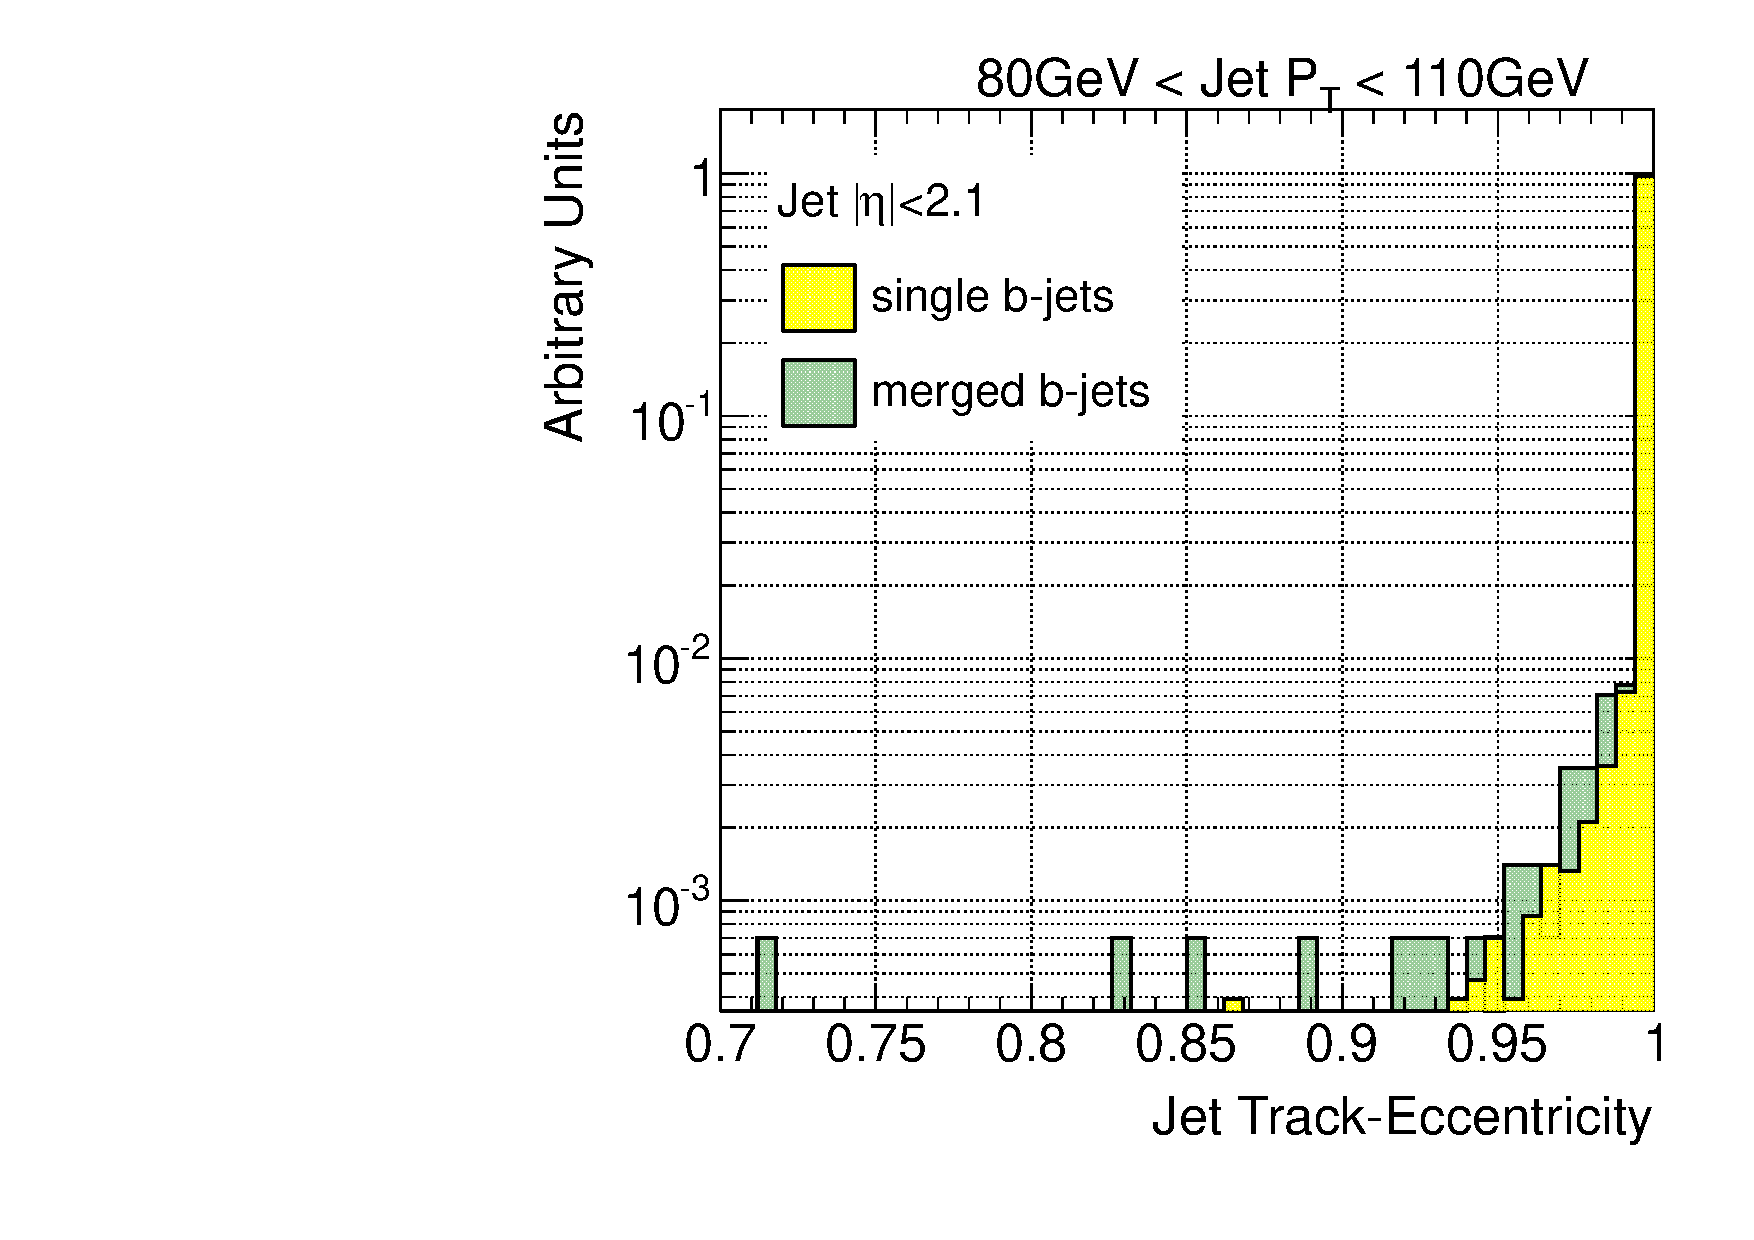
\includegraphics[width=0.49\textwidth]{FIGS/TEMPFigs/Antikt6VarsSingleMerged/JetTrackEccentricity080.pdf}
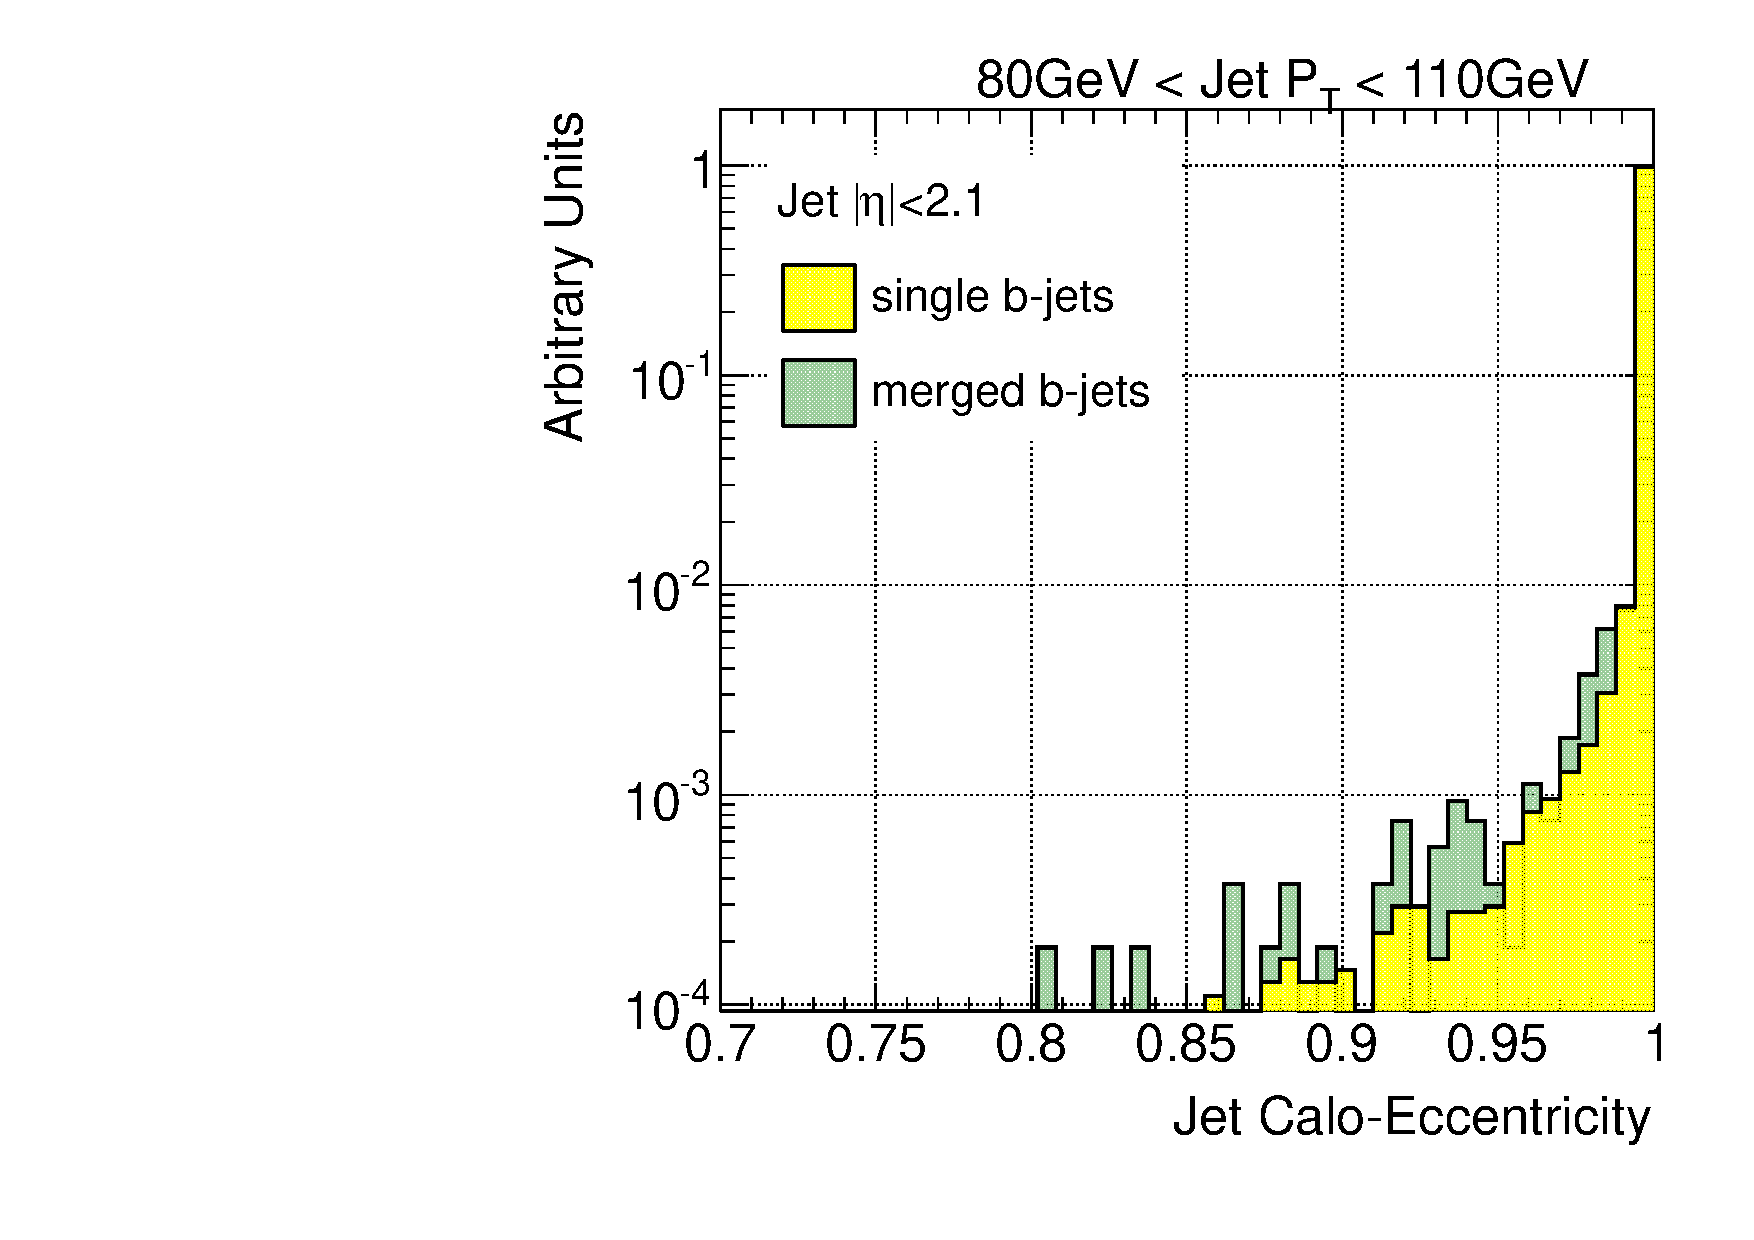
\includegraphics[width=0.49\textwidth]{FIGS/TEMPFigs/GhostMatchingVarsClus/JetCaloEccentricity080.pdf}
\caption{Distribution of the jet eccentricity for single and merged $b$-jets between 80~GeV to 110~GeV in anti-$k_T$ 0.6 jets using track constituents (left) and anti-$k_T$ 0.4 jets using the active area of the jet, with calorimeter topoclusters as input.}
\label{fig:jeteccGhostAndAntikt6}
\end{figure}




%------------------------------------------------------------------------
\section{Validation of the jet variables in data}\label{sec:gbbValidation}
%------------------------------------------------------------------------

 In order to study the extent to which the simulation reproduces the distributions observed in data for the different variables explored a set of comparison plots is presented. Figures~\ref{fig:datamcinputvars} and~\ref{fig:datamcinputvars2} show distributions of jet track multiplicity, track-jet width, $\Delta R$ between the axes of the two $k_t$ subjets, $\max\{\Delta R(trk,trk)\}$ and $\tau_2$ in two different $\pt$ bins for $b$-tagged jets in dijet Monte Carlo and data events passing selection described in Section~\ref{sec:EventSelection}.
The distributions are normalized to unit area to allow for shape comparisons. There is a good agreement between data and simulation. 

It should be remarked that the observed agreement is actually not a direct validation of the description in the MC of the relevant variables, but its convolution with the simulated relative fractions of light-, $c$-, $b$- and $bb$-jets in the $b$-tagged generated jet sample. To some extent, there could be some level of compensation between these two effects, although the agreement evaluated in $b$-jets selected with a looser cut of MV1 tagger as well as with another $b$-tagging algorithm is still ver good, suggesting that this compasation is not likely to occur in samples sufficiently enriched in $b$-jets.


\begin{figure}[tp]
\centering
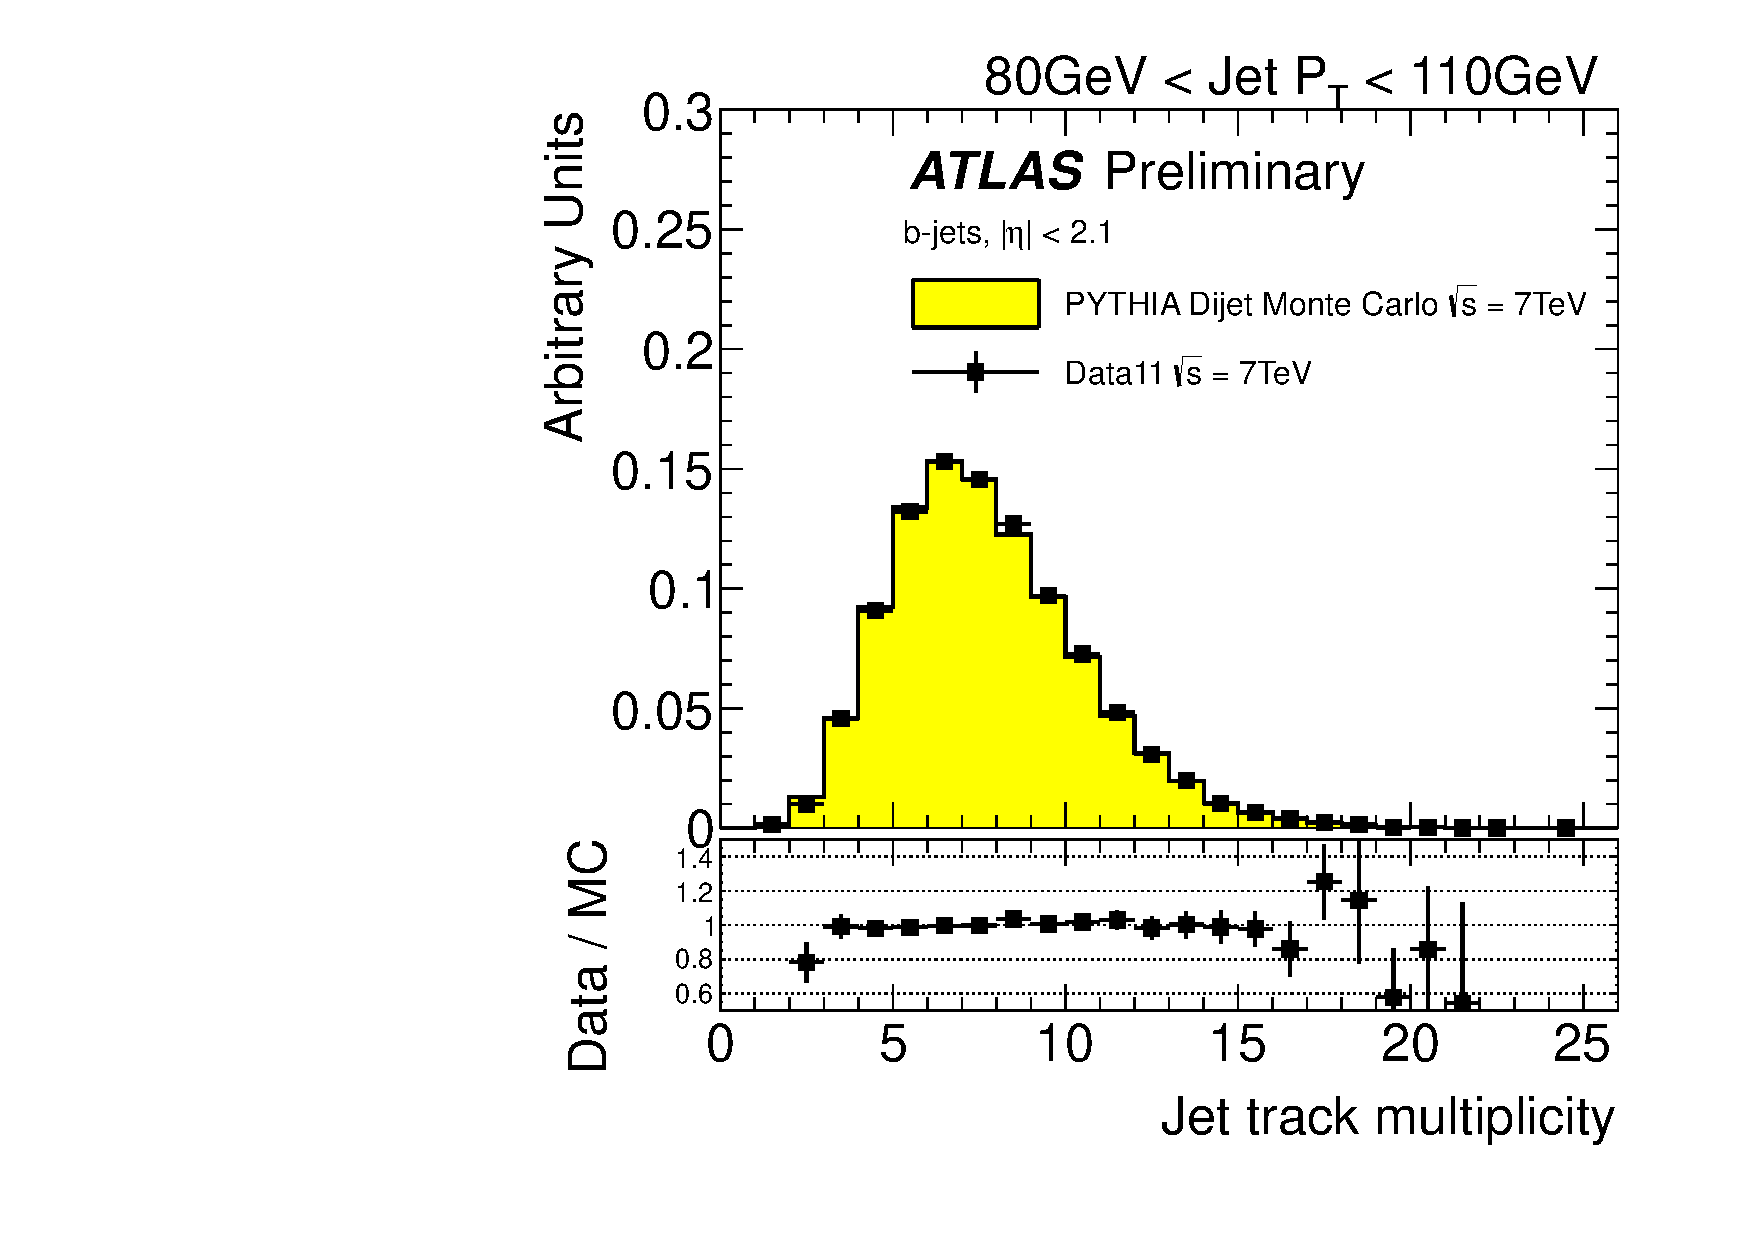
\includegraphics[width=0.49\textwidth]{FIGS/dataMC/FullDataVarNtrkPT080.pdf}
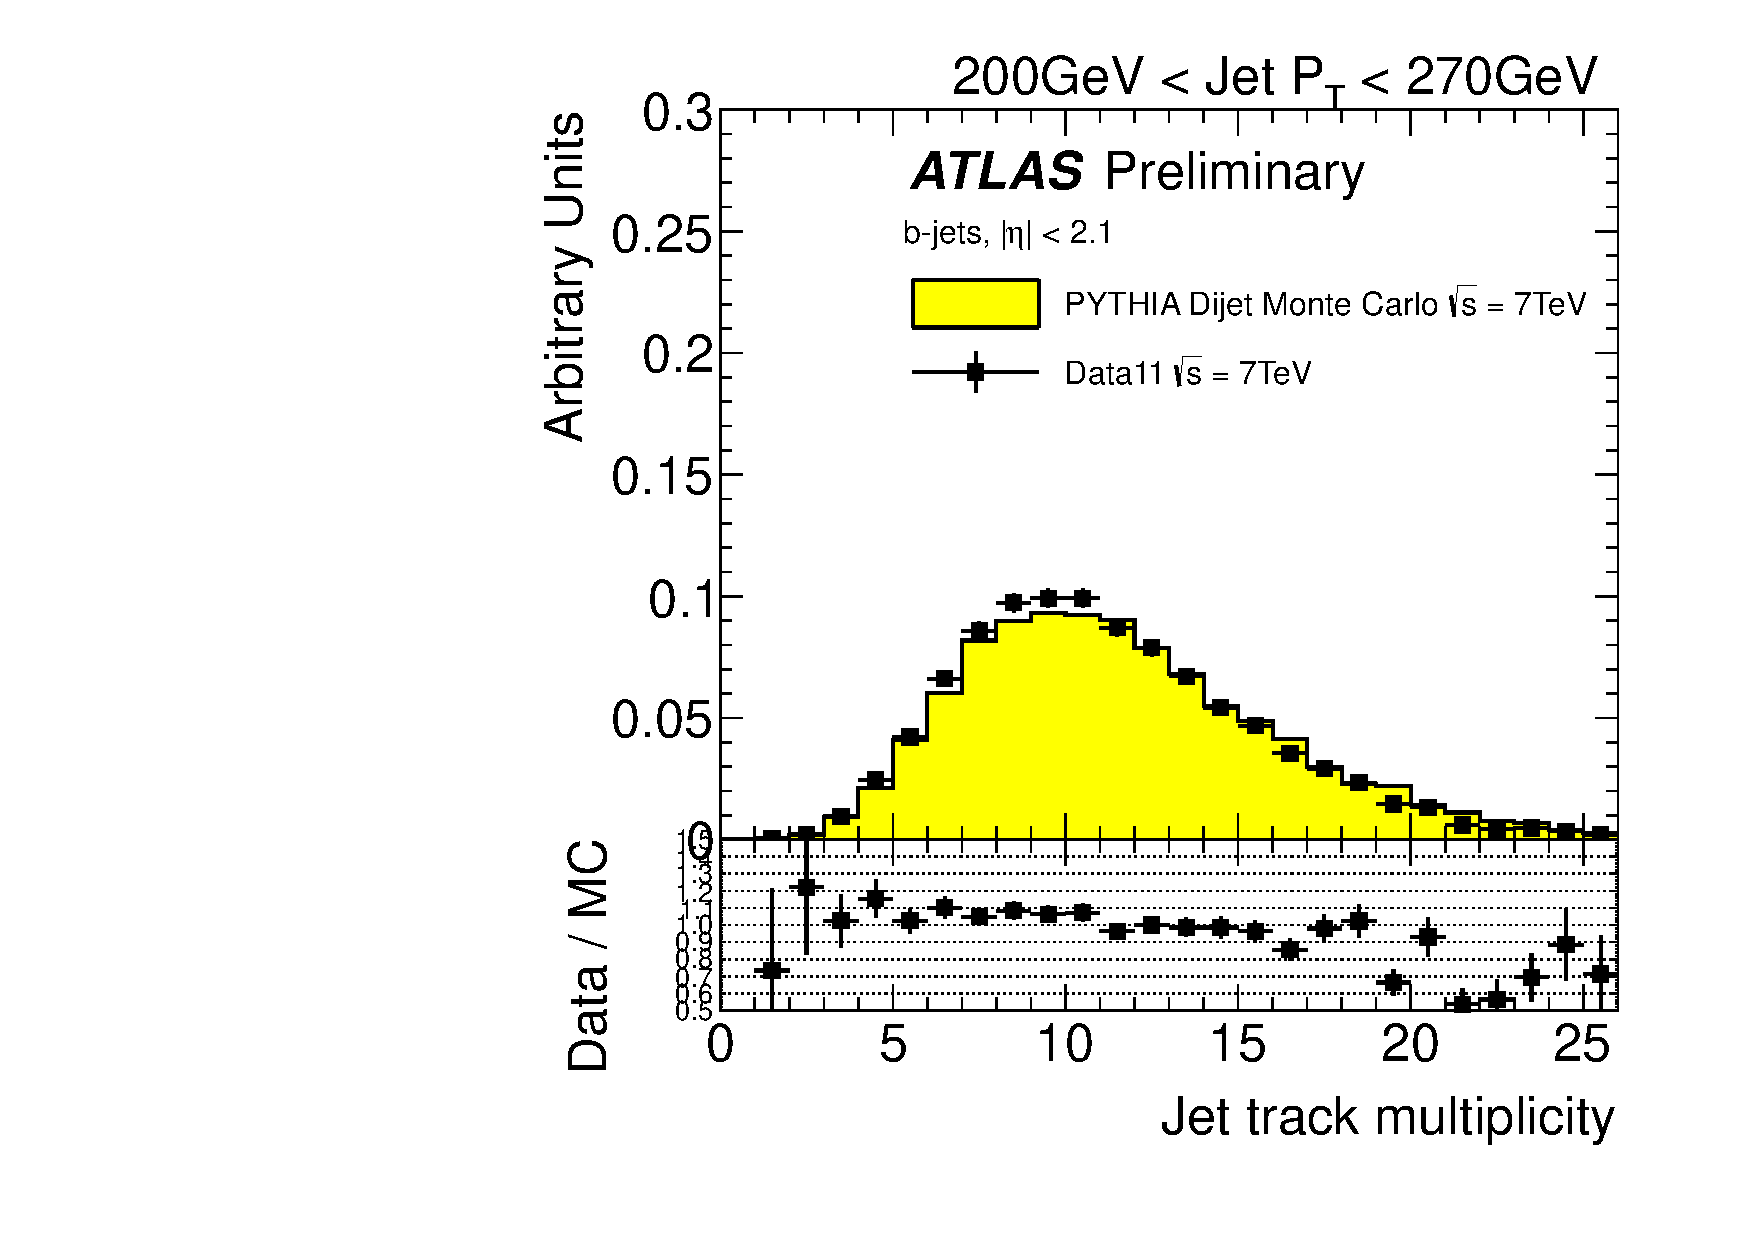
\includegraphics[width=0.49\textwidth]{FIGS/dataMC/FullDataVarNtrkPT200.pdf}
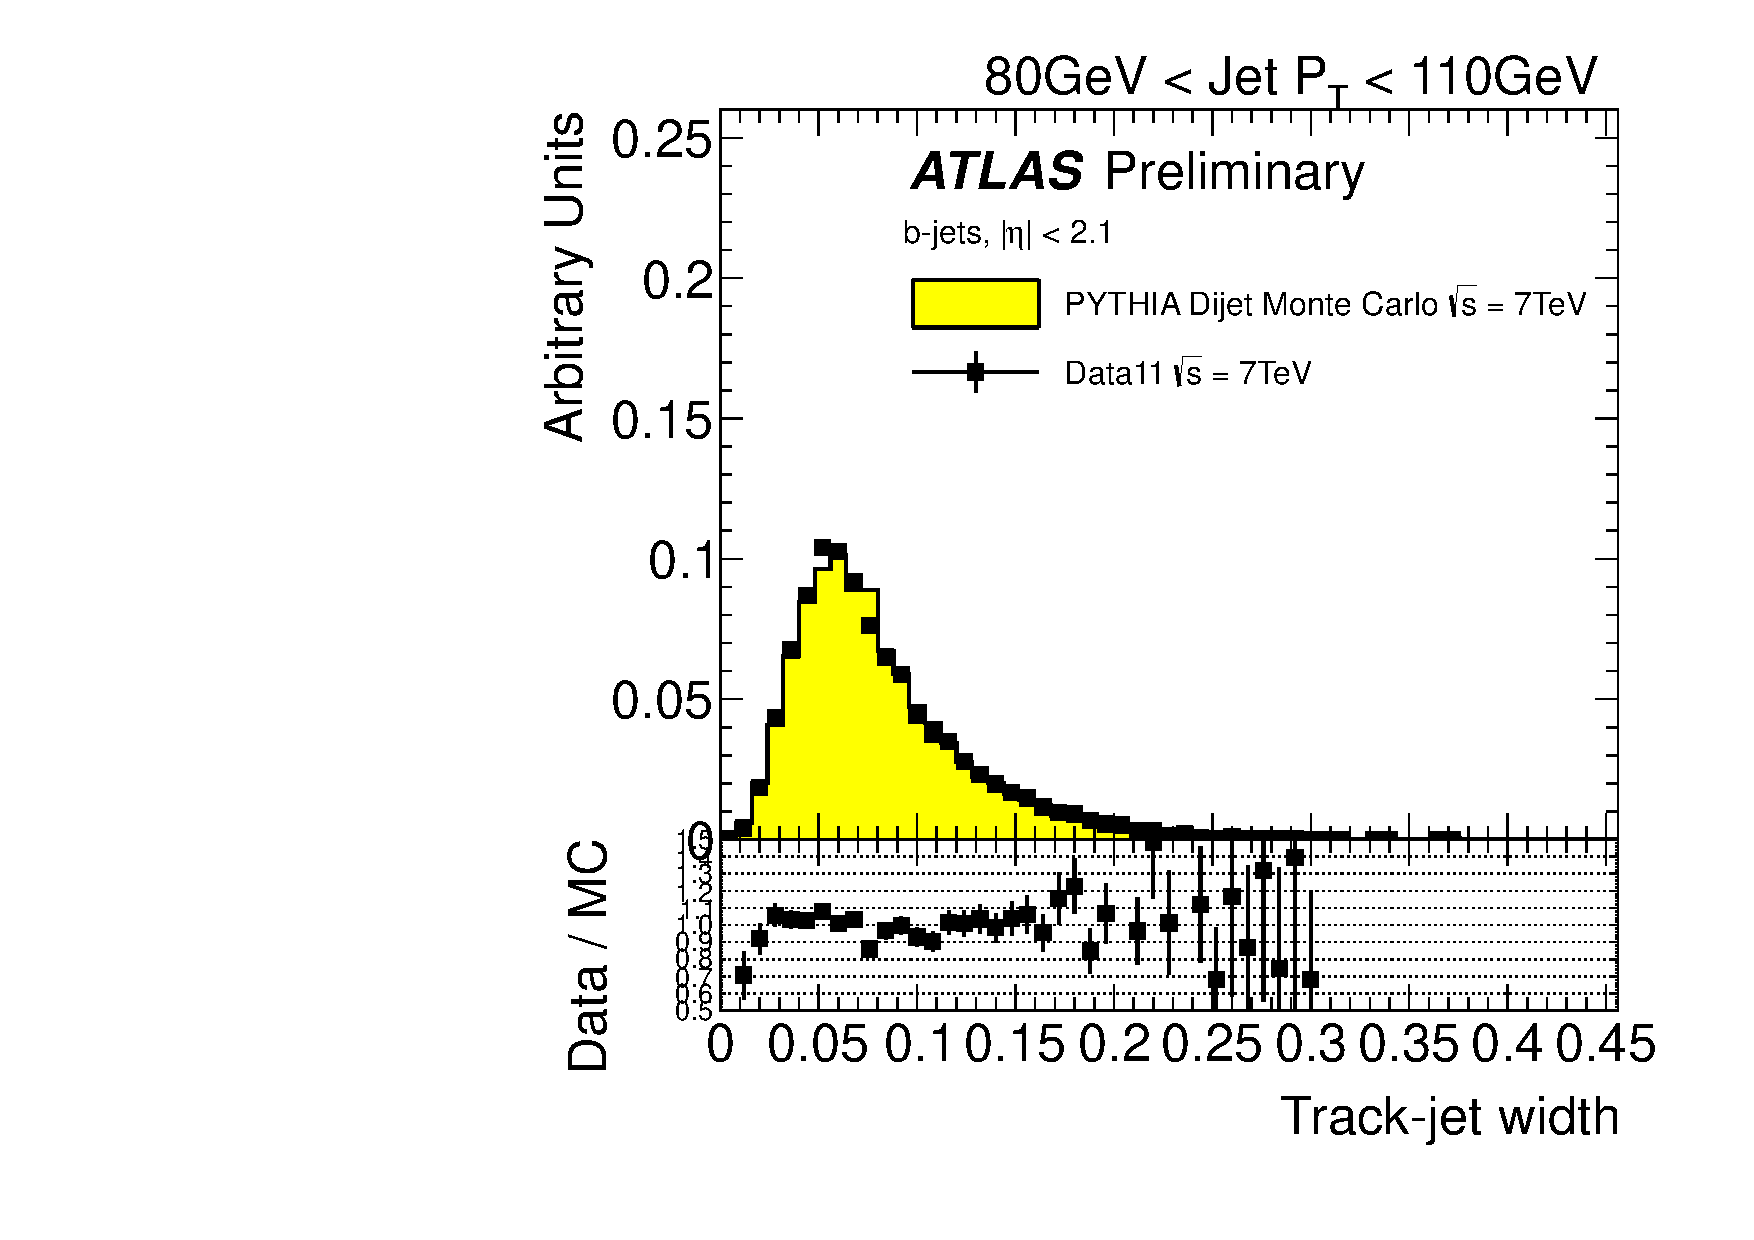
\includegraphics[width=0.49\textwidth]{FIGS/dataMC/FullDataVarTrkWidthPT080.pdf}
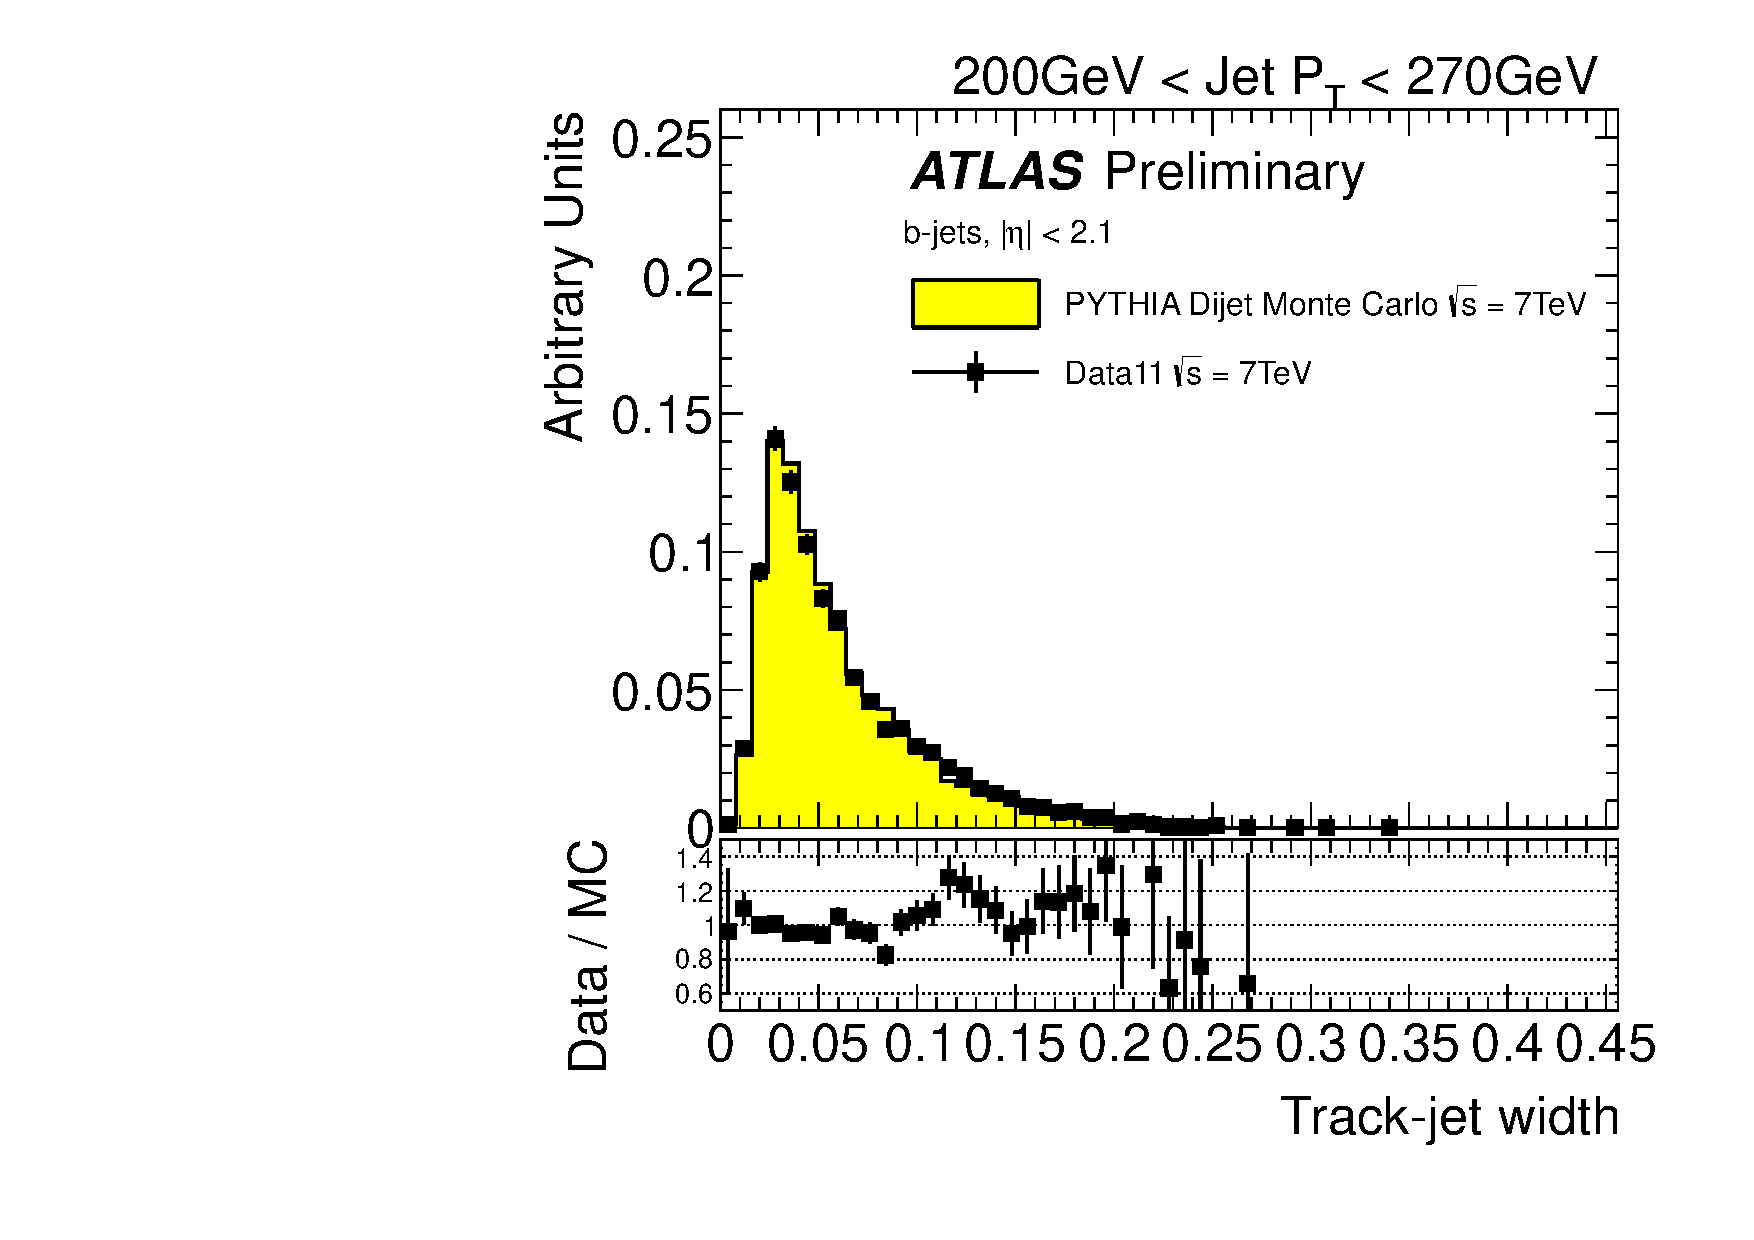
\includegraphics[width=0.49\textwidth]{FIGS/dataMC/FullDataVarTrkWidthPT200.pdf}  
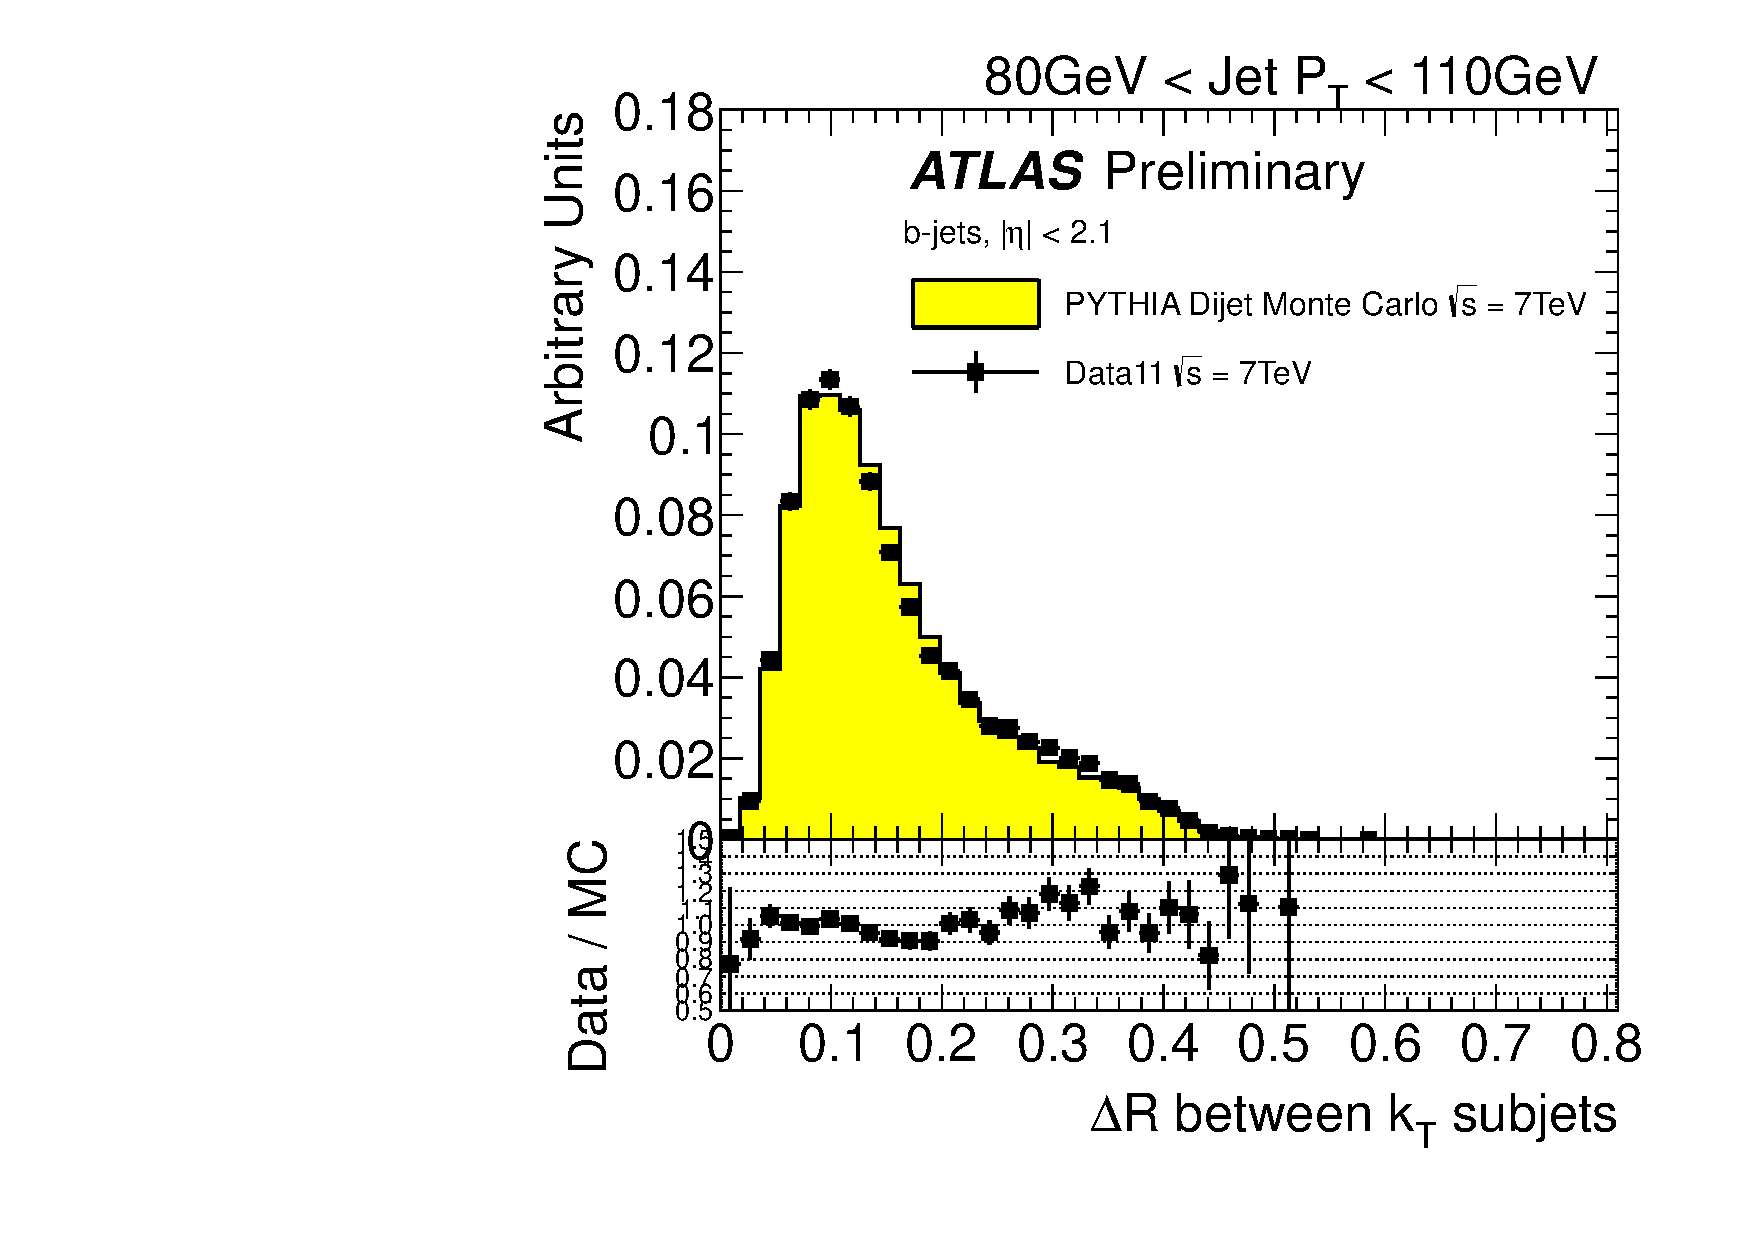
\includegraphics[width=0.49\textwidth]{FIGS/dataMC/FullDataVarDRktaxisPT080.pdf}
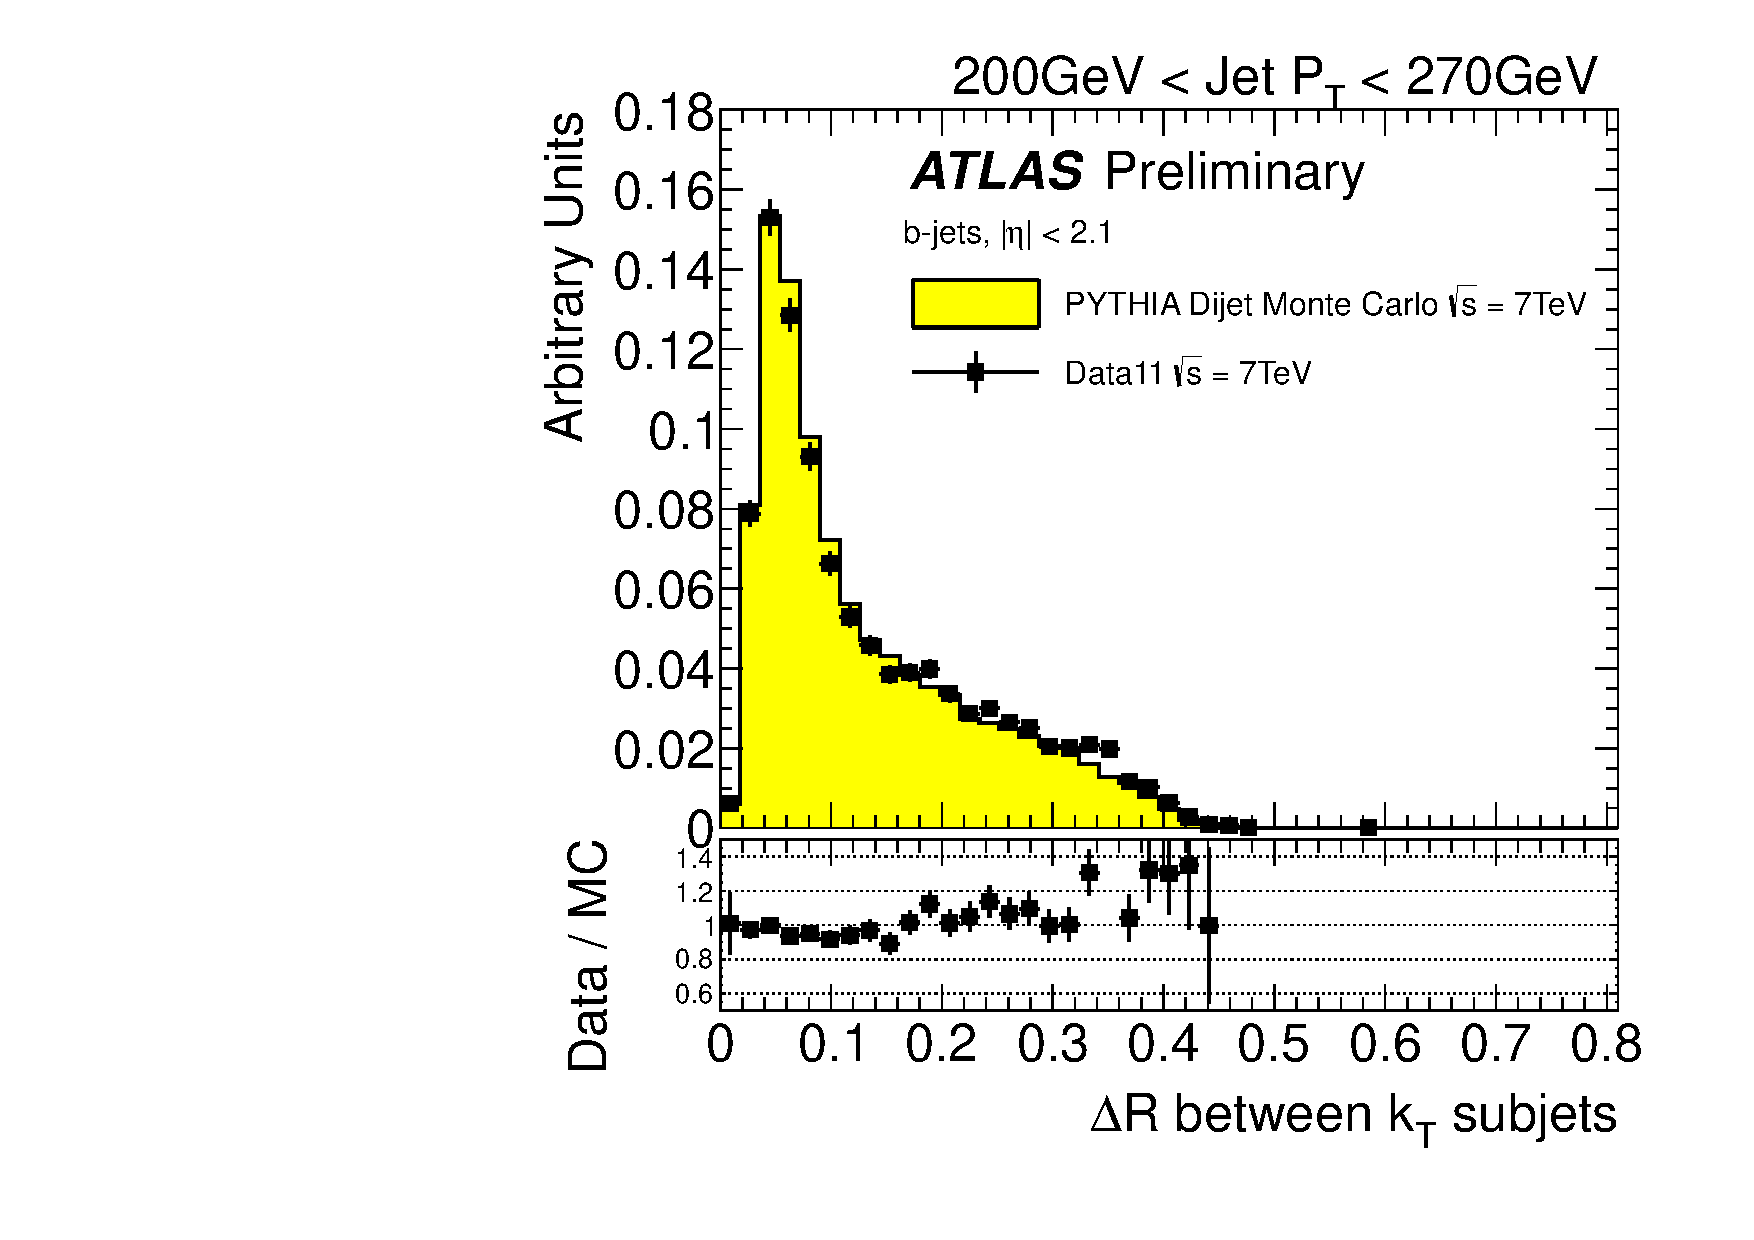
\includegraphics[width=0.49\textwidth]{FIGS/dataMC/FullDataVarDRktaxisPT200.pdf}  
%\caption{ Distribution of three tracking variables in 2 different jet $\pt$ bins, for experimental data  collected by ATLAS until summer 2011, with $\mu \approx 6$ (solid black points), and simulated data (filled histograms). The ratio data over simulation is shown at the bottom of each plot.}
\caption{ Distribution of three tracking variables in 2 different jet $\pt$ bins, for experimental data  collected by ATLAS during 2011 (solid black points), and simulated data (filled histograms). The ratio data over simulation is shown at the bottom of each plot.}
\label{fig:datamcinputvars}
\end{figure}

\begin{figure}[tp]
\centering
\includegraphics[width=0.49\textwidth]{FIGS/dataMC/FullDataVarDRmaxPT080.pdf}
\includegraphics[width=0.49\textwidth]{FIGS/dataMC/FullDataVarDRmaxPT200.pdf}
\includegraphics[width=0.49\textwidth]{FIGS/dataMC/FullDataVarTau2PT080.pdf}
\includegraphics[width=0.49\textwidth]{FIGS/dataMC/FullDataVarTau2PT200.pdf}  
\caption{ Distribution of two tracking variables in two different jet $\pt$ bins, for experimental data  collected by ATLAS during 2011 (solid black points), and simulated data (filled histograms). The ratio data over simulation is shown at the bottom of each plot.}
\label{fig:datamcinputvars2}
\end{figure}



